\chapter{Resultados Complementarios de la Aplicación al Tráfico}
\label{aneC_00_00_trafico}

% Corridas 101 (rezago {1}) y 102 (rezagos {1, 7}), M = 10, test, w = 30 salvo indicación.
% Cuadros desde reports/reales/real_trafico_10{1,2}_v01_barrido_M/{98,99}_* y desde los .npz del _04;
% figuras de §3, §5 y §6 redibujadas con el estilo del Capítulo 3 (scratchpad figuras_trafico.py); el resto, del _01/_04.

Este anexo reúne los resultados de la aplicación al tráfico del Capítulo~\ref{04_00_00_aplicacion} que no se reportan en el cuerpo, para las dos especificaciones que se comparan, la que usa el rezago de un día, $\{1\}$, y la que agrega el de una semana, $\{1,7\}$. Salvo indicación, las cifras corresponden a $M = 10$, al bloque de prueba y a la ventana móvil de ancho $w = 30$.

\section{Configuración de la aplicación}
\label{aneC_00_01_configuracion}

El Cuadro~\ref{tab:aneC_configuracion} recoge la configuración con que se ajustaron las dos especificaciones. Lo que no se indica coincide con el estudio de simulación (Anexo~\ref{ane_00_03_configuracion}); las diferencias son la representación, que aquí se estima, el hiperparámetro de forma $a_\nu$, la inclusión a priori de los rezagos y el número de cadenas.

\begin{table}[H]
\centering\small
\caption{Configuración de la aplicación al tráfico.}
\label{tab:aneC_configuracion}
\begin{tabular}{p{0.22\textwidth} p{0.40\textwidth} p{0.30\textwidth}}
\hline
Elemento & Descripción & Valor \\
\hline
Datos & Metro Interstate Traffic Volume (UCI), estación ATR 301, I-94 oeste & Volumen horario, miles de veh./h \\
Ventana & Días de la serie / horas por día & 1 jul 2015 a 30 sep 2018, $T = 1188$ / $G = 24$ \\
Partición & Entrenamiento / prueba & 831 / 357 días ($T_0 = 831$) \\
Representación & B-spline cúbica ajustada a las horas observadas & $J = 10$ \\
FPCA & Componentes retenidas, estimadas en entrenamiento & $M = 10$ \\
Covariables & Scores de $t-1$ / de $t-1$ y $t-7$ & $d = 10$ / $d = 20$ \\
$N$, $L_j$ & Truncamiento y grilla de localización & $30$, $50$ \\
Muestreador & Cadenas / iteraciones / descartadas & $1$ / $2500$ / $1000$ \\
$a_\nu$, $a_\varkappa$, $b_\varkappa$ & Forma de las precisiones y de la contracción & $2$, $0.5$, $0.5$ \\
$(a_{\varpi_j}, b_{\varpi_j})$ & Inclusión, todos los rezagos & $(1, 5)$ \\
FAR($p$) & Orden igual al mayor rezago & $p = 1$ / $p = 7$ \\
Random Forest & Rezagos elegidos con el entrenamiento & Entre $\{1\}$ y $\{1,7\}$ \\
Ventana de detalle & Diez días con más días no laborables & 23 dic 2017 a 1 ene 2018 ($t = 907$ a $916$) \\
\hline
\end{tabular}
\end{table}

Las constantes de los comportamientos son las del Cuadro~\ref{tab:dis_comportamientos}, sin recorte de las extracciones, porque con $a_\nu = 2$ la varianza de los átomos es finita.

\section{Datos y representación}
\label{aneC_00_02_datos}
% Mismos días en 101 y 102: figuras de la 102_01 (01-10).

La serie diaria, sus momentos, la representación en la base B-spline y la FPCA son comunes a las dos especificaciones.

\begin{figure}[H]
\centering
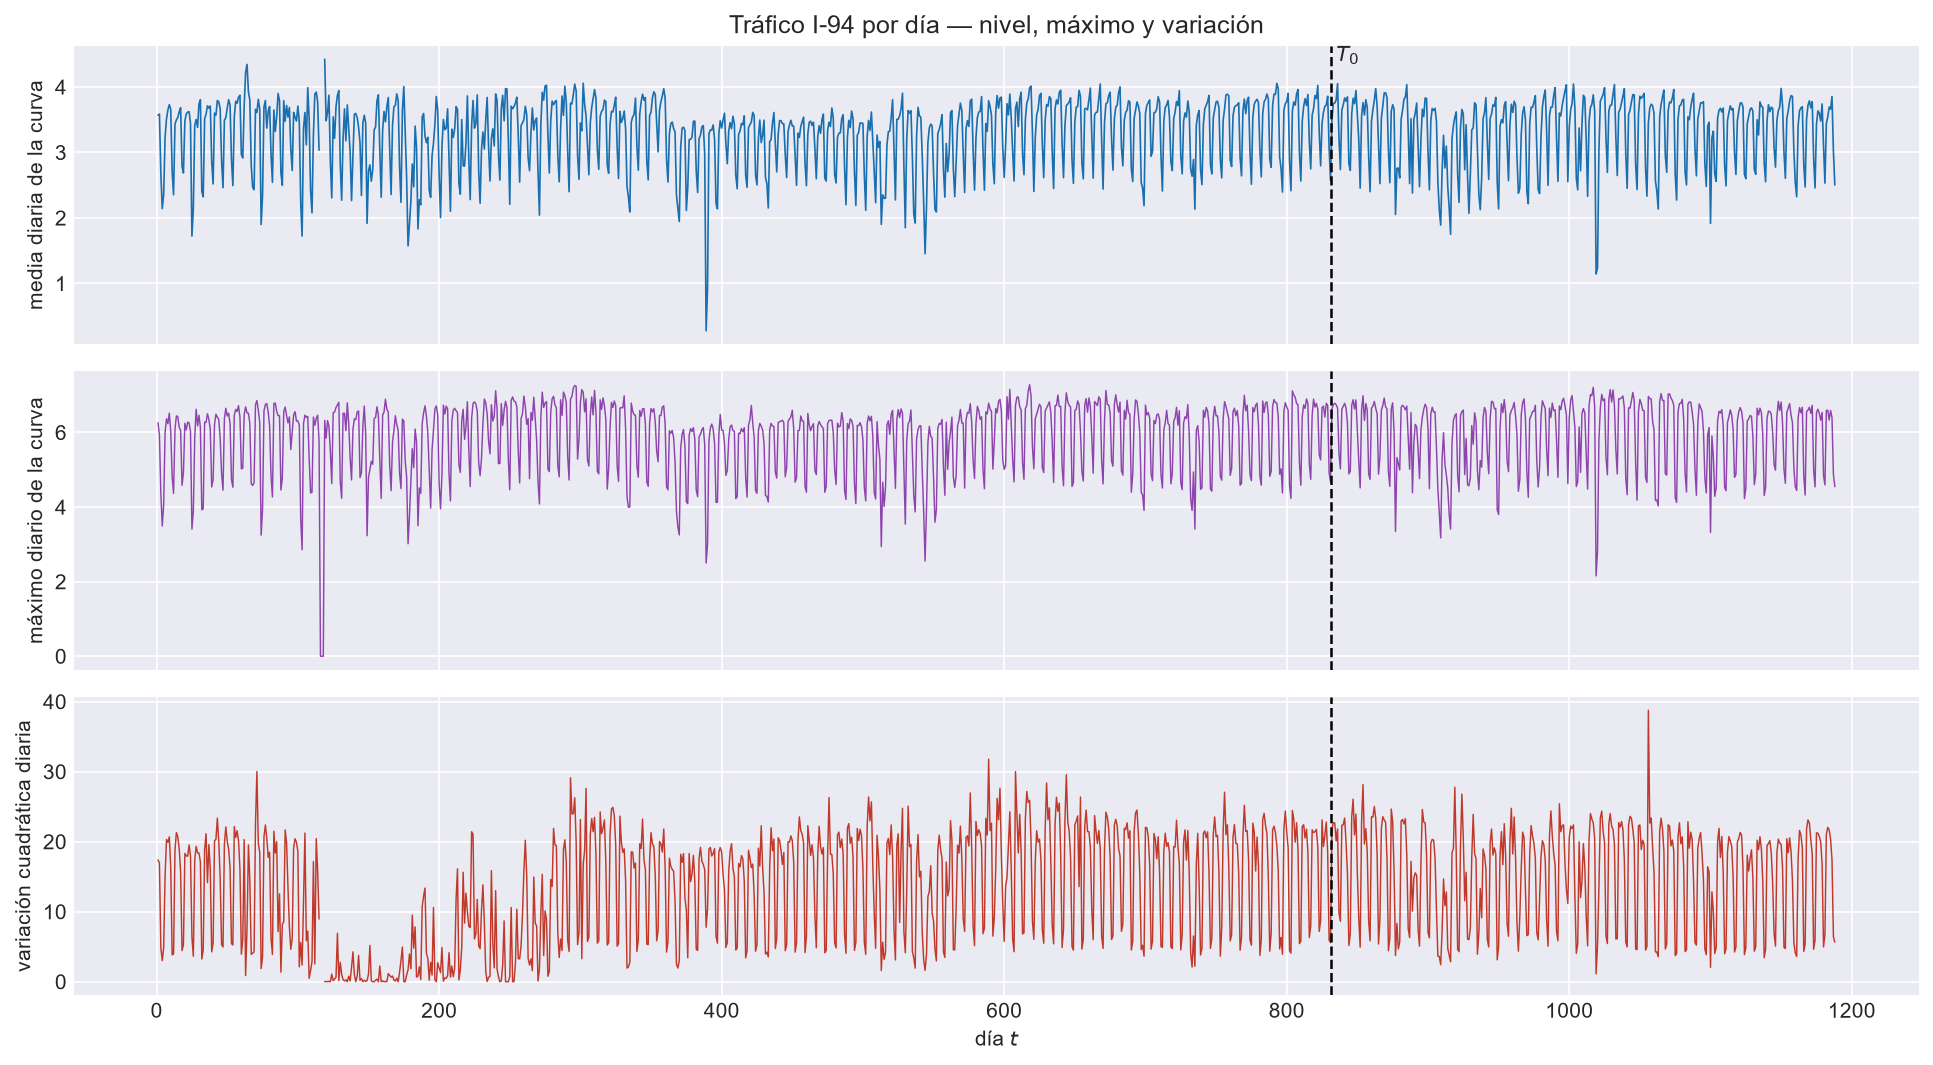
\includegraphics[width=\textwidth,height=0.7\textheight,keepaspectratio]{IMG/aneC_00/aneC_00_04_serie_diaria.png}
\caption{Serie diaria del volumen de tráfico.}
\label{fig:aneC_04_serie_diaria}
\end{figure}

\begin{figure}[H]
\centering
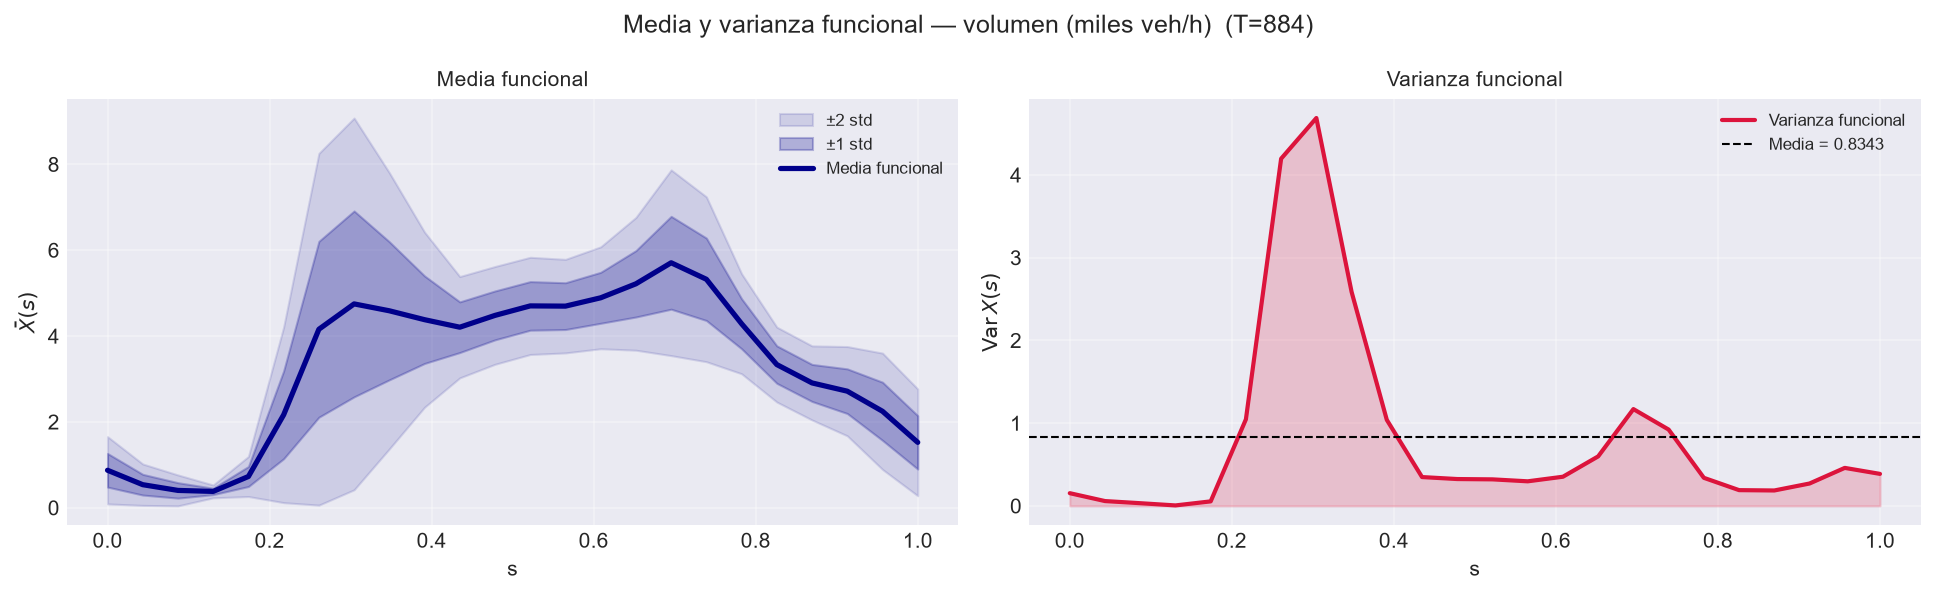
\includegraphics[width=\textwidth,height=0.7\textheight,keepaspectratio]{IMG/aneC_00/aneC_00_03_media_varianza_raw.png}
\caption{Media y varianza de la curva diaria.}
\label{fig:aneC_03_media_varianza_raw}
\end{figure}

\begin{figure}[H]
\centering
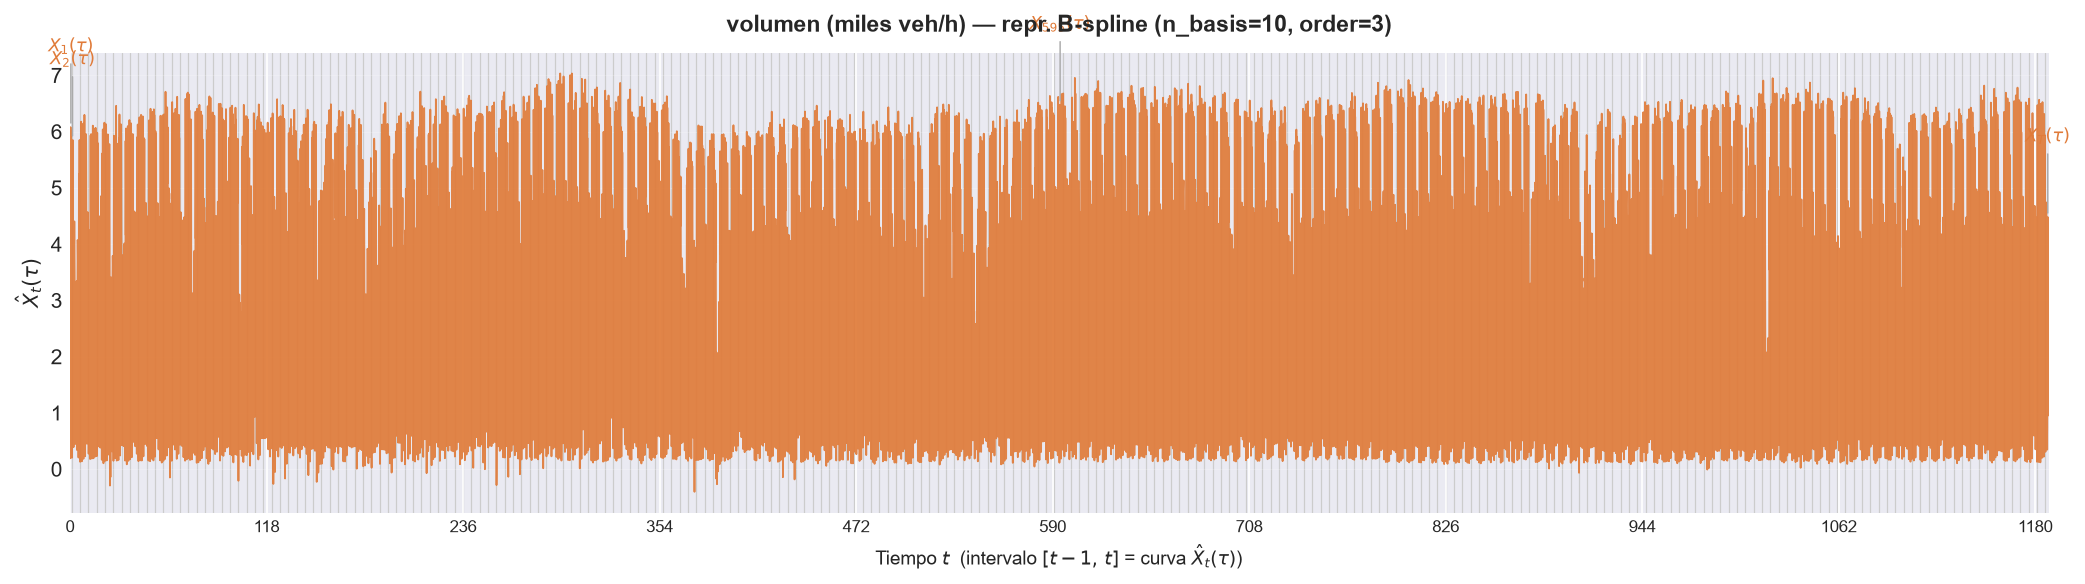
\includegraphics[width=\textwidth,height=0.7\textheight,keepaspectratio]{IMG/aneC_00/aneC_00_06_fts_funcional_bspline.png}
\caption{Curvas diarias en la base B-spline con $J = 10$.}
\label{fig:aneC_06_fts_funcional_bspline}
\end{figure}

\begin{figure}[H]
\centering
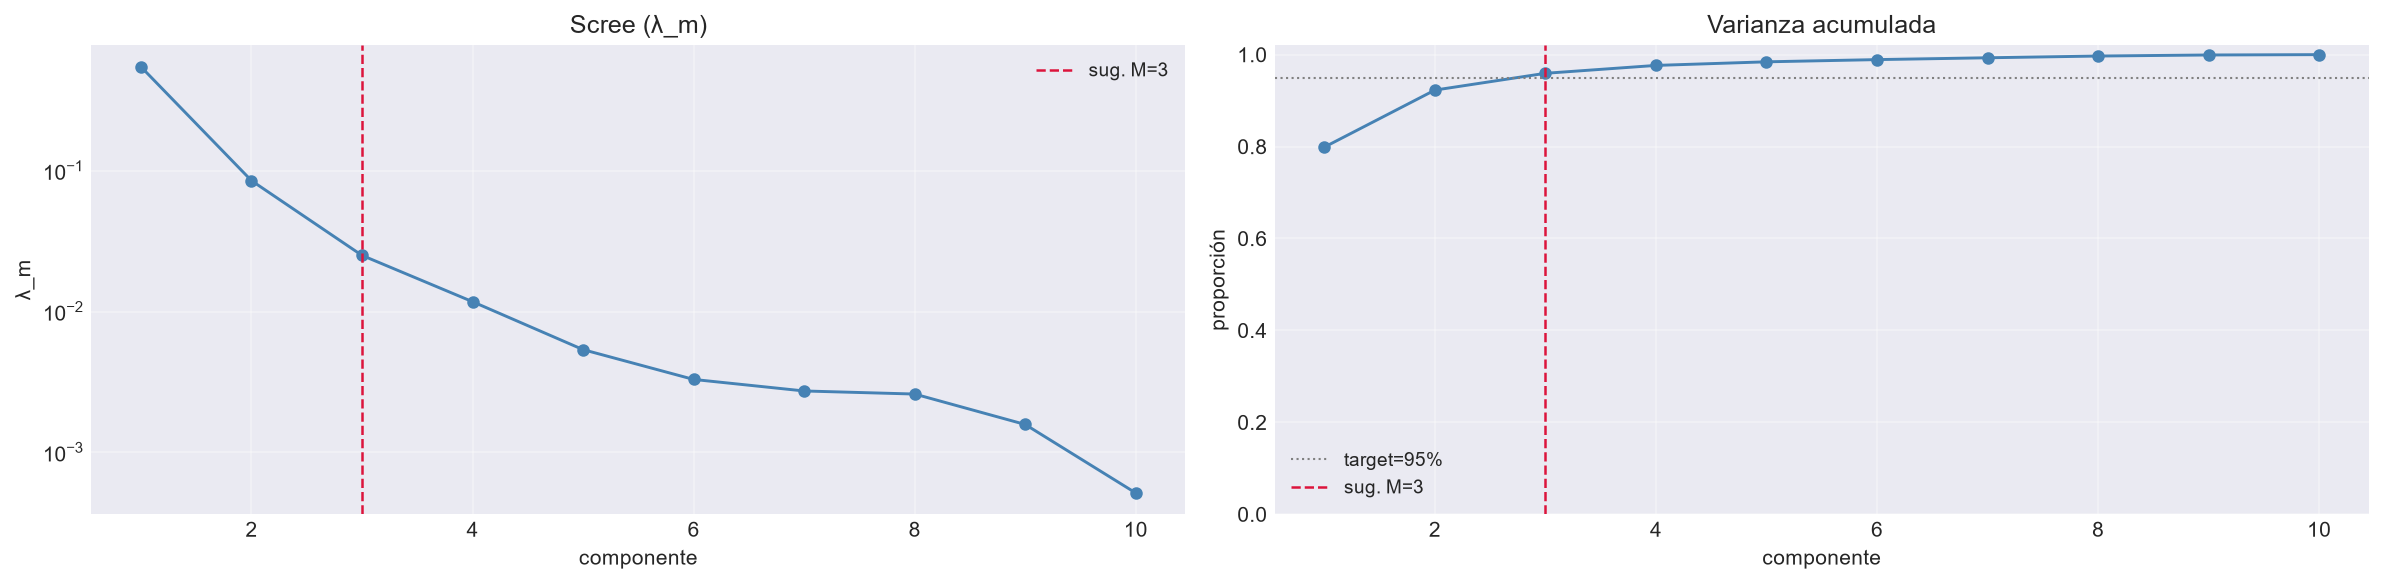
\includegraphics[width=\textwidth,height=0.7\textheight,keepaspectratio]{IMG/aneC_00/aneC_00_07_fpca_scree.png}
\caption{Varianza explicada por componente de la FPCA (bloque de entrenamiento).}
\label{fig:aneC_07_fpca_scree}
\end{figure}

\begin{figure}[H]
\centering
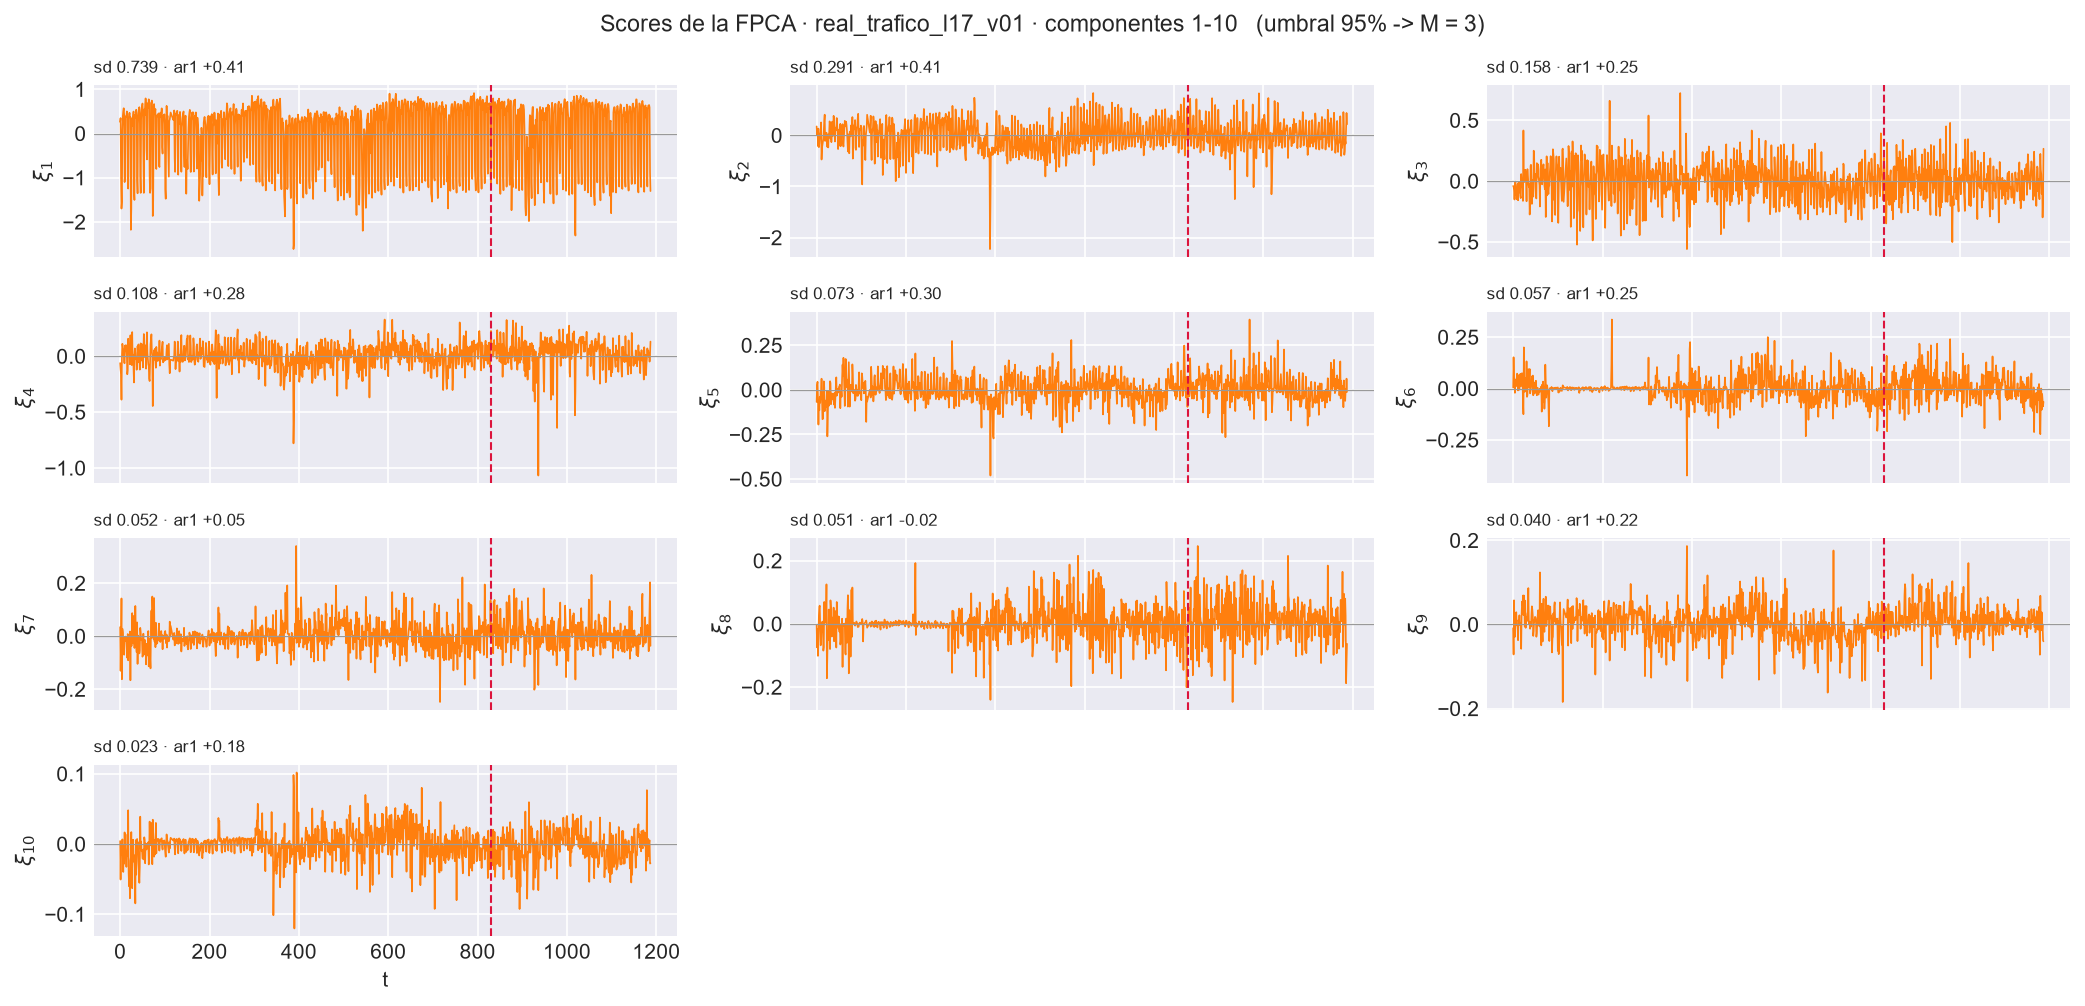
\includegraphics[width=\textwidth,height=0.7\textheight,keepaspectratio]{IMG/aneC_00/aneC_00_07b_series_scores.png}
\caption{Series de scores de la FPCA.}
\label{fig:aneC_07b_series_scores}
\end{figure}

\begin{figure}[H]
\centering
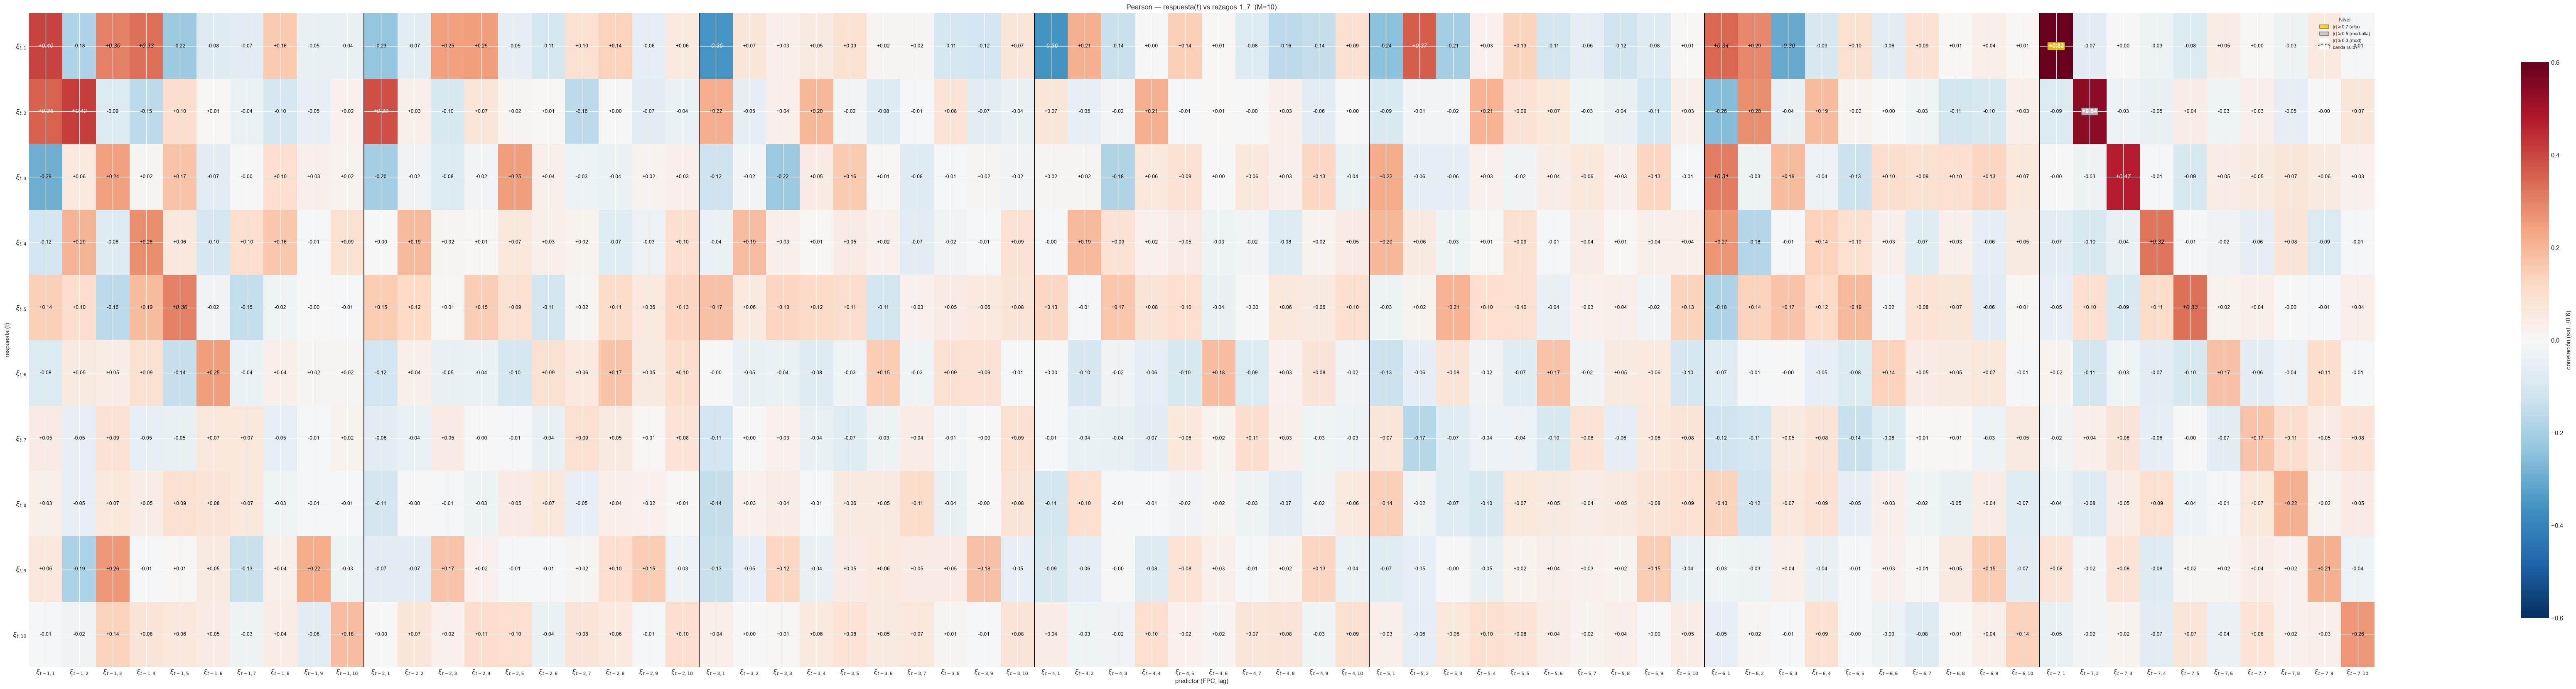
\includegraphics[width=\textwidth,height=0.7\textheight,keepaspectratio]{IMG/aneC_00/aneC_00_09a_rezagos_pearson.png}
\caption{Autocorrelación de los scores por rezago (Pearson).}
\label{fig:aneC_09a_rezagos_pearson}
\end{figure}

\begin{figure}[H]
\centering
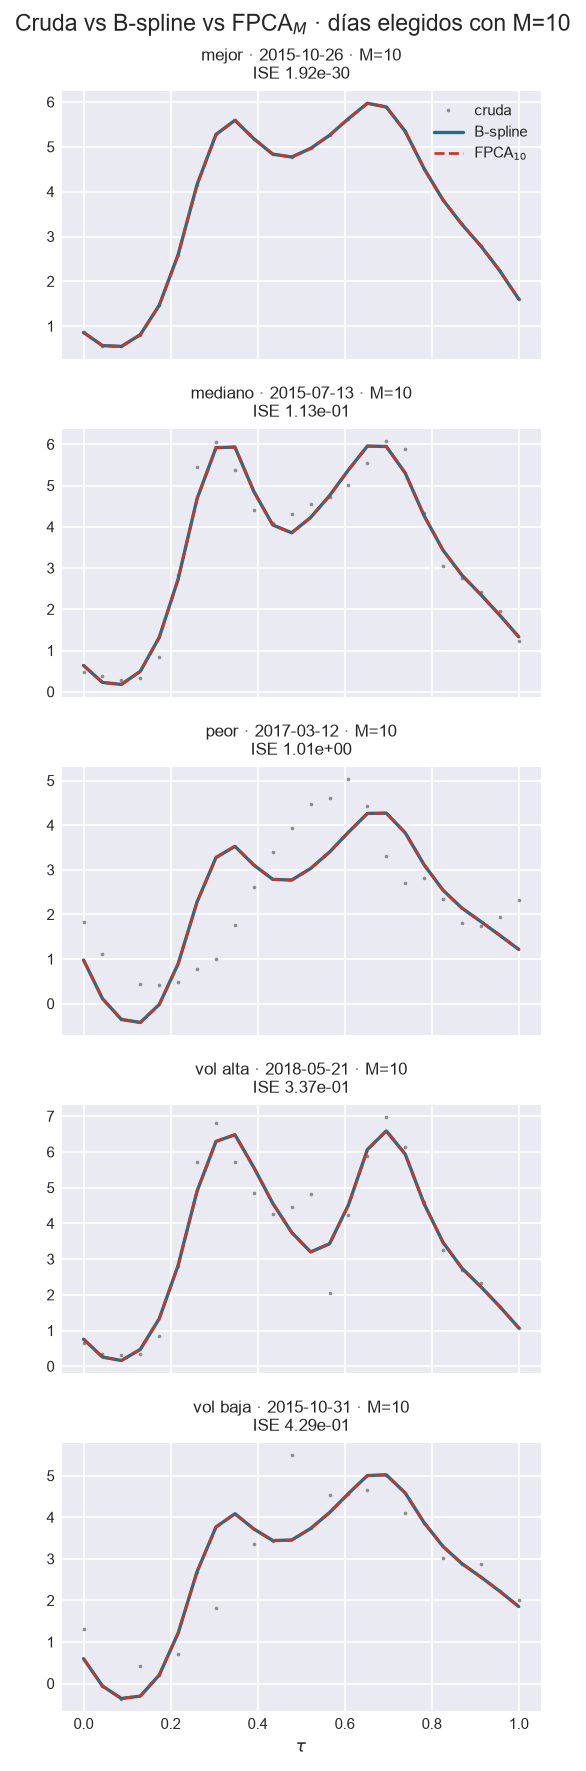
\includegraphics[width=\textwidth,height=0.7\textheight,keepaspectratio]{IMG/aneC_00/aneC_00_10_tres_curvas.png}
\caption{Tres curvas observadas y su representación con $M = 10$.}
\label{fig:aneC_10_tres_curvas}
\end{figure}

\section{Métricas completas}
\label{aneC_00_03_metricas}

Las diez métricas del Marco Teórico en el bloque de prueba, como promedio sobre las ventanas de ancho $w = 30$.
% Fuente: 98_resumen_bloqueA_min_max_prom.csv de 101 y 102 (test, M = 10).
\begin{table}[H]
\centering\small
\caption{Métricas de error en el bloque de prueba del tráfico ($M = 10$, $w = 30$).}
\label{tab:aneC_A}
\begin{tabular}{l l cccc}
\hline
Rezagos & Modelo & MAE & RMSE & $\overline{\mathrm{E}}_{\max}$ & $\mathrm{E}_{\max}^{\mathrm{glob}}$ \\
\hline
$\{1\}$   & PSBPM-FD, esperanza          & 0.413 & 0.646 & 1.241 & 3.347 \\
          & PSBPM-FD, mediana puntual    & 0.376 & 0.658 & 1.147 & 3.999 \\
          & PSBPM-FD, átomo más probable & 0.397 & 0.729 & 1.198 & 4.385 \\
          & FAR                          & 0.398 & 0.621 & 1.224 & 3.102 \\
          & Random Forest                & 0.361 & 0.562 & 1.076 & 3.000 \\
\hline
$\{1,7\}$ & PSBPM-FD, esperanza          & 0.315 & 0.522 & 0.906 & 3.367 \\
          & PSBPM-FD, mediana puntual    & 0.302 & 0.528 & 0.879 & 3.628 \\
          & PSBPM-FD, átomo más probable & 0.317 & 0.556 & 0.920 & 3.859 \\
          & FAR                          & 0.314 & 0.495 & 0.897 & 3.106 \\
          & Random Forest                & 0.314 & 0.499 & 0.896 & 3.076 \\
\hline
\end{tabular}
\end{table}

% Fuente: 99_resumen_bloqueB_min_max_prom.csv de 101 y 102 (test, M = 10).
\begin{table}[H]
\centering\small
\setlength{\tabcolsep}{4pt}
\caption{Métricas de intervalo en el bloque de prueba del tráfico ($M = 10$, $w = 30$). Nivel nominal $0.95$.}
\label{tab:aneC_B}
\begin{tabular}{l l cccccc}
\hline
Rezagos & Banda & MPIW & PICP & PICPB & Winkler & $\overline{\mathrm{W}}_{\max}$ & $\mathrm{W}_{\max}^{\mathrm{glob}}$ \\
\hline
$\{1\}$   & Equi-colas      & 2.124 & 0.961 & 0.731 & 2.734 & 7.845 & 43.392 \\
          & Máxima densidad & 1.995 & 0.960 & 0.742 & 2.669 & 7.422 & 46.019 \\
          & Simultánea      & 4.242 & 0.991 & 0.942 & 4.493 & 9.717 & 33.688 \\
          & FAR             & 2.159 & 0.950 & 0.721 & 3.073 & 9.253 & 50.983 \\
\hline
$\{1,7\}$ & Equi-colas      & 1.752 & 0.956 & 0.754 & 2.707 & 8.041 & 67.843 \\
          & Máxima densidad & 1.689 & 0.955 & 0.746 & 2.714 & 7.918 & 70.530 \\
          & Simultánea      & 3.011 & 0.983 & 0.917 & 3.549 & 7.831 & 55.352 \\
          & FAR             & 1.602 & 0.930 & 0.675 & 3.052 & 9.922 & 78.072 \\
\hline
\end{tabular}
\end{table}

\begin{figure}[H]
\centering
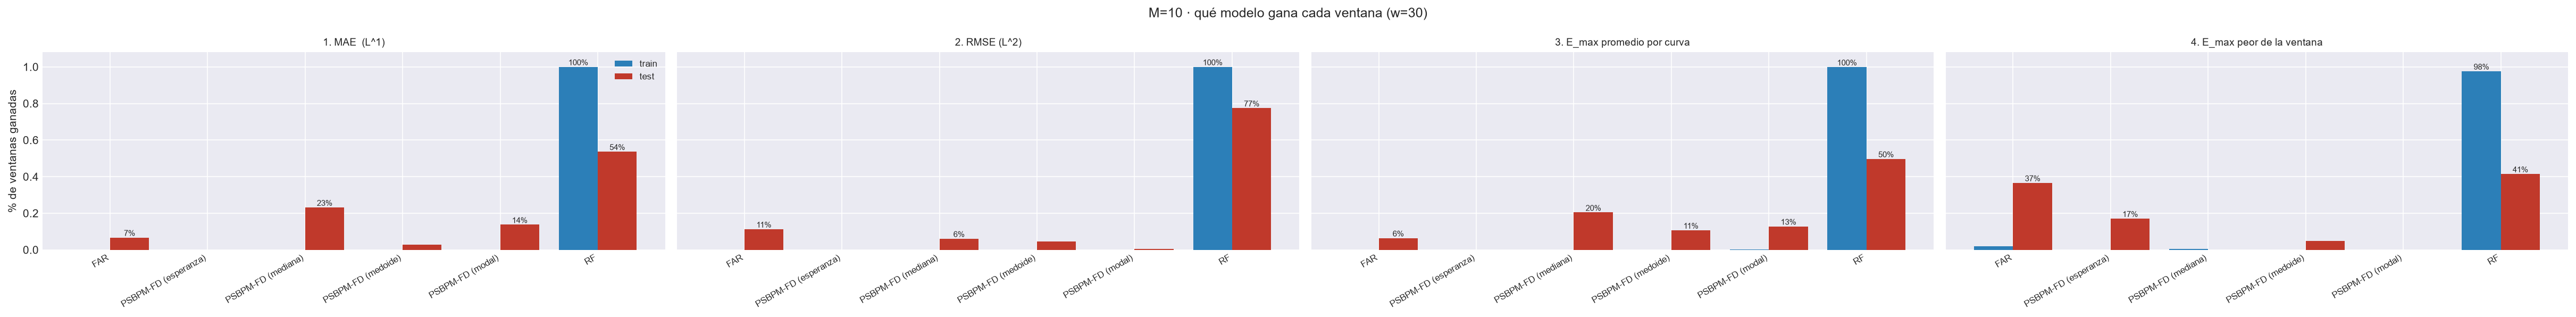
\includegraphics[width=\textwidth,height=0.75\textheight,keepaspectratio]{IMG/aneC_00/aneC_00_78_ganador_ventana_bloqueA_101.png}
\caption{Modelo con menor MAE en cada ventana, tráfico con rezago $\{1\}$ ($M = 10$).}
\label{fig:aneC_78_ganador_ventana_bloqueA_101}
\end{figure}

\begin{figure}[H]
\centering
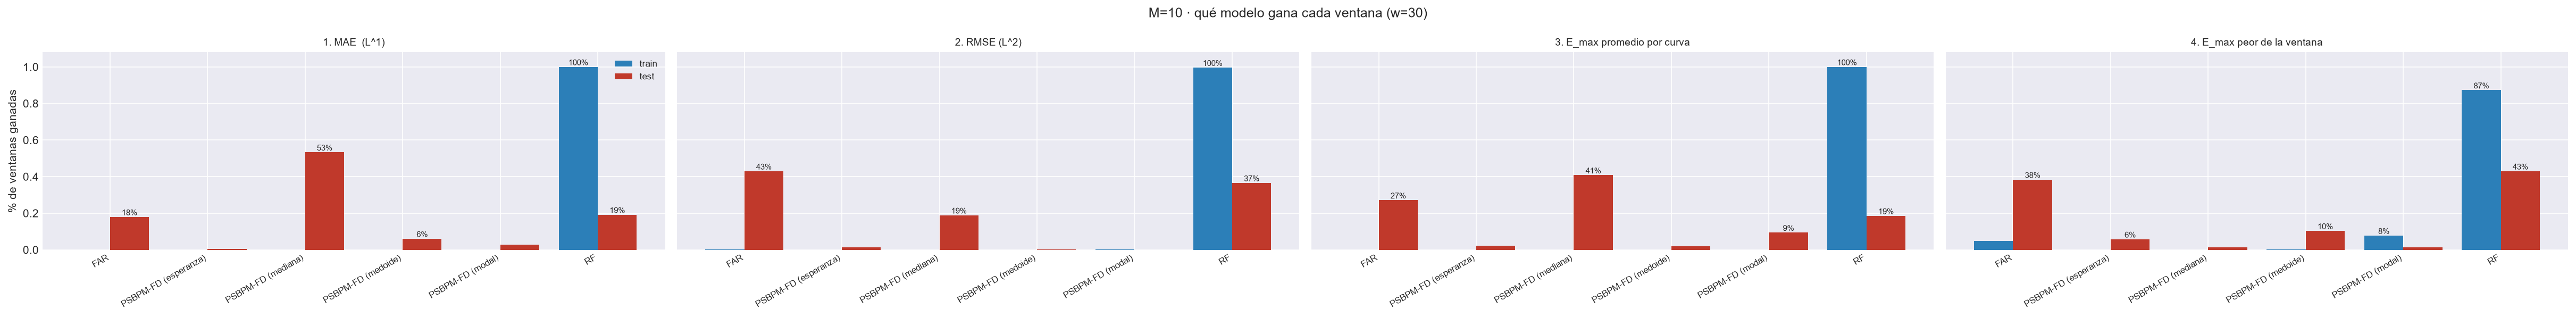
\includegraphics[width=\textwidth,height=0.75\textheight,keepaspectratio]{IMG/aneC_00/aneC_00_78_ganador_ventana_bloqueA_102.png}
\caption{Modelo con menor MAE en cada ventana, tráfico con rezagos $\{1,7\}$ ($M = 10$).}
\label{fig:aneC_78_ganador_ventana_bloqueA_102}
\end{figure}

\section{Sensibilidad al ancho de la ventana}
\label{aneC_00_04_ventana}

Las métricas de error y de intervalo sobre la ventana móvil con $w = 20$ y $w = 40$; el Capítulo~\ref{04_00_00_aplicacion} reporta $w = 30$. Las métricas de intervalo se muestran para las tres construcciones del PSBPM-FD.

% Fuente: 72_ventana_modelos_w{20,40}.csv del _05 y ventana móvil de las bandas de banda_funcional_psbp.npz,
% recalculada con la llamada del _04 (con w = 30 reproduce 81_ventana_bloqueB_w30.csv a 1e-14).
\begin{figure}[H]
\centering
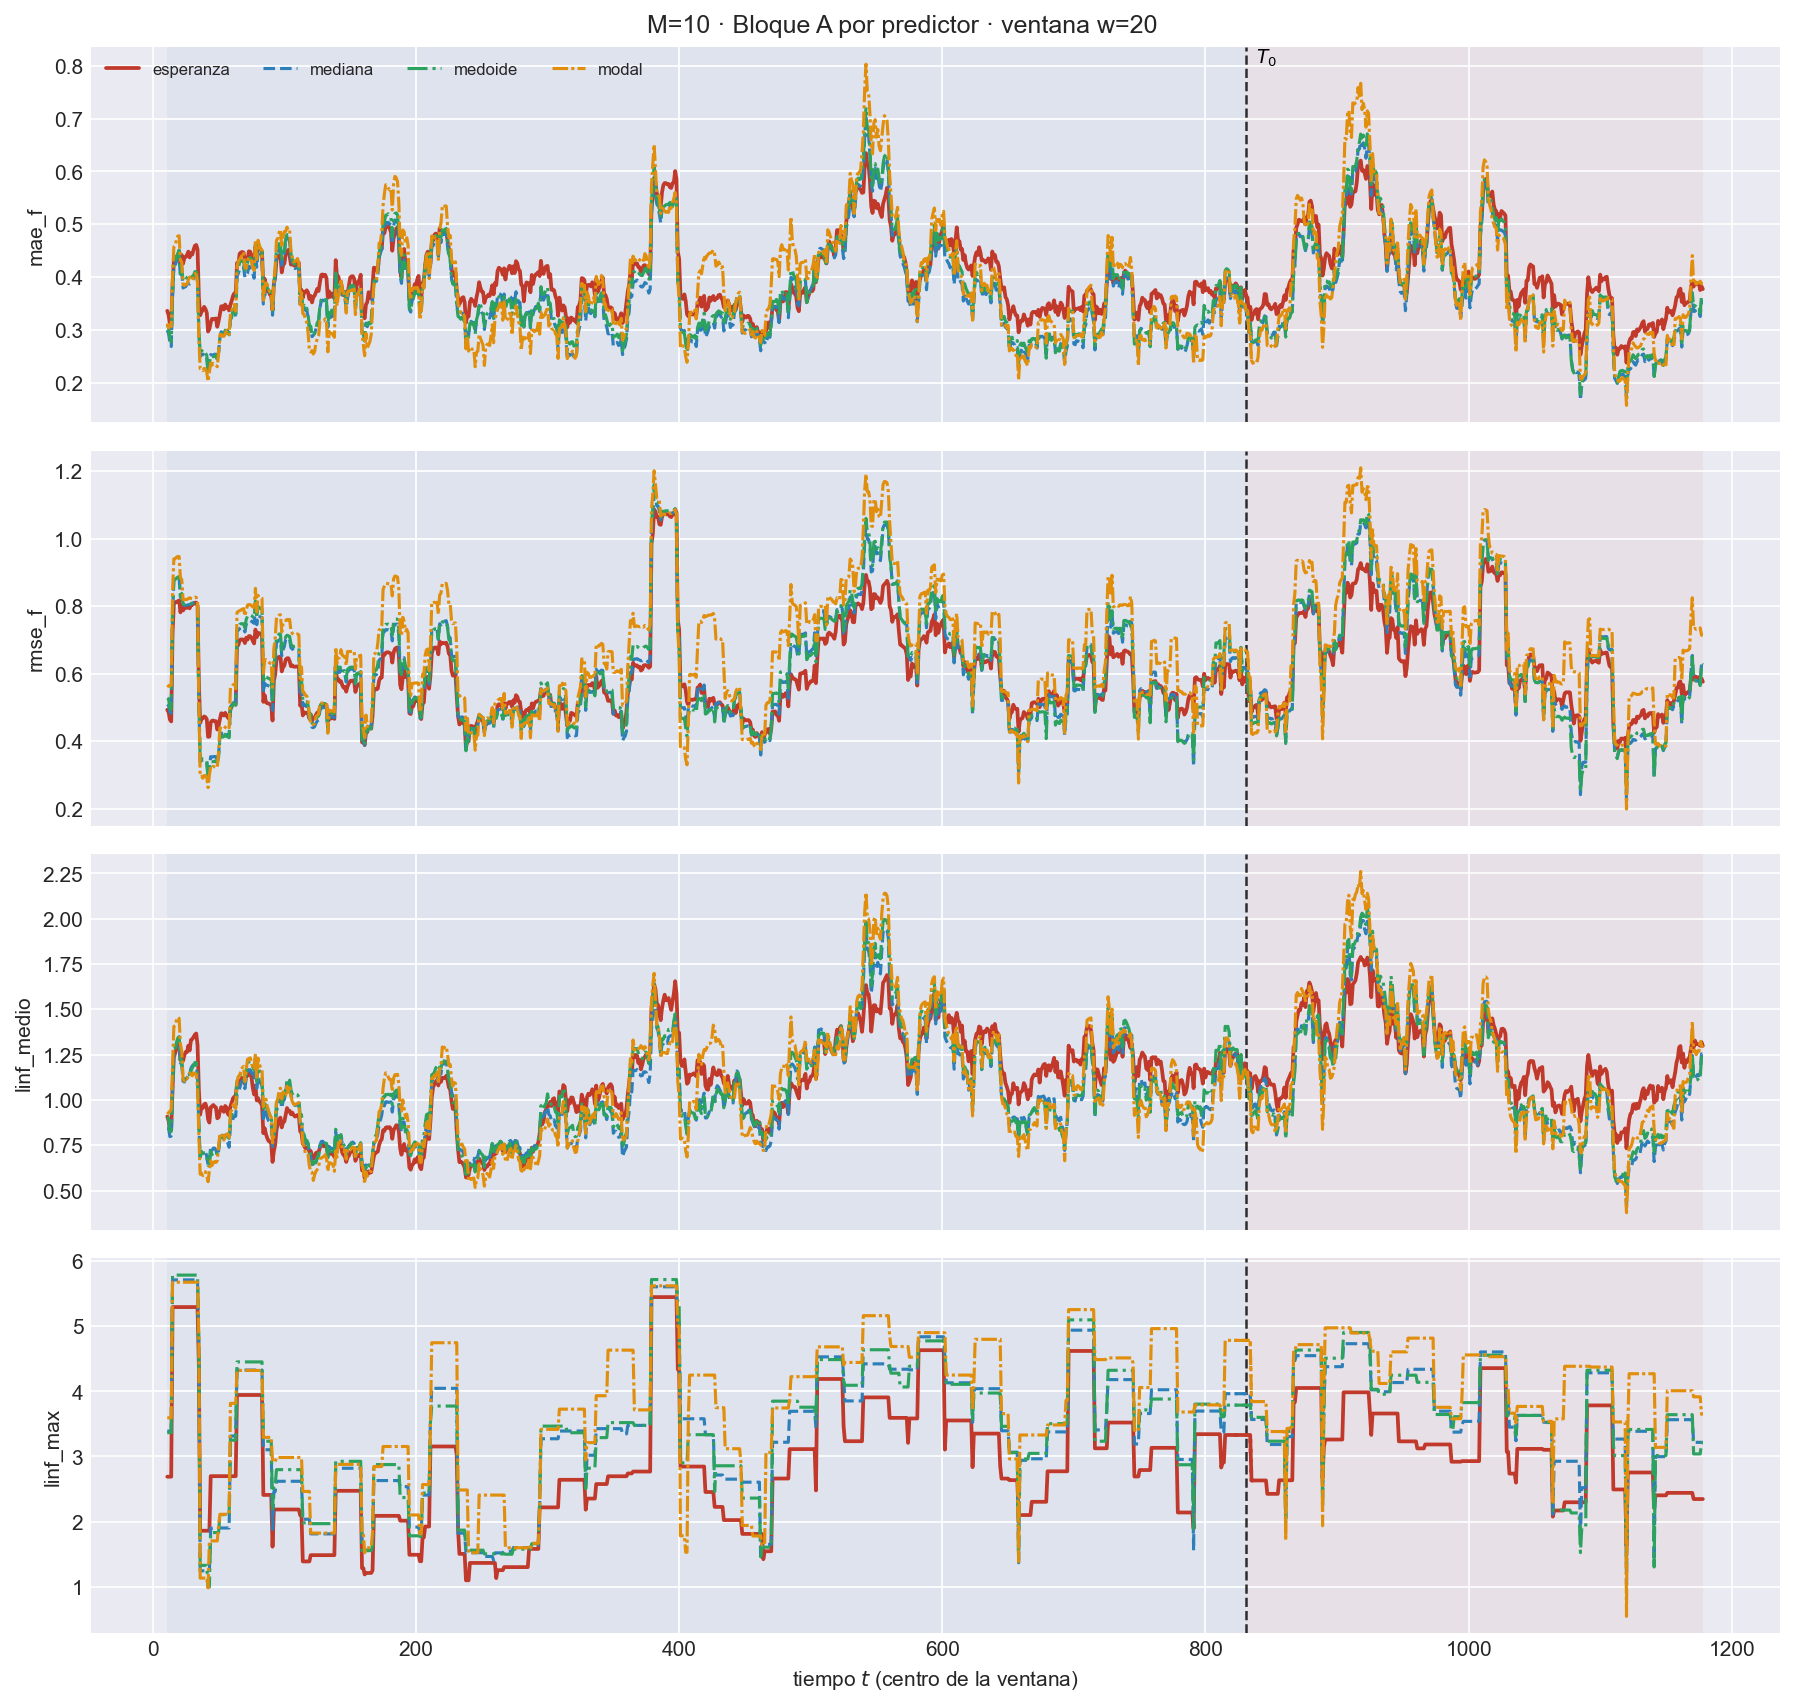
\includegraphics[width=\textwidth]{IMG/aneC_00/aneC_00_58_ventana_predictores_w20_101.png}
\caption{Métricas de error sobre la ventana móvil con $w = 20$, tráfico con rezago $\{1\}$ ($M = 10$).}
\label{fig:aneC_58_ventana_predictores_w20_101}
\end{figure}

\begin{figure}[H]
\centering
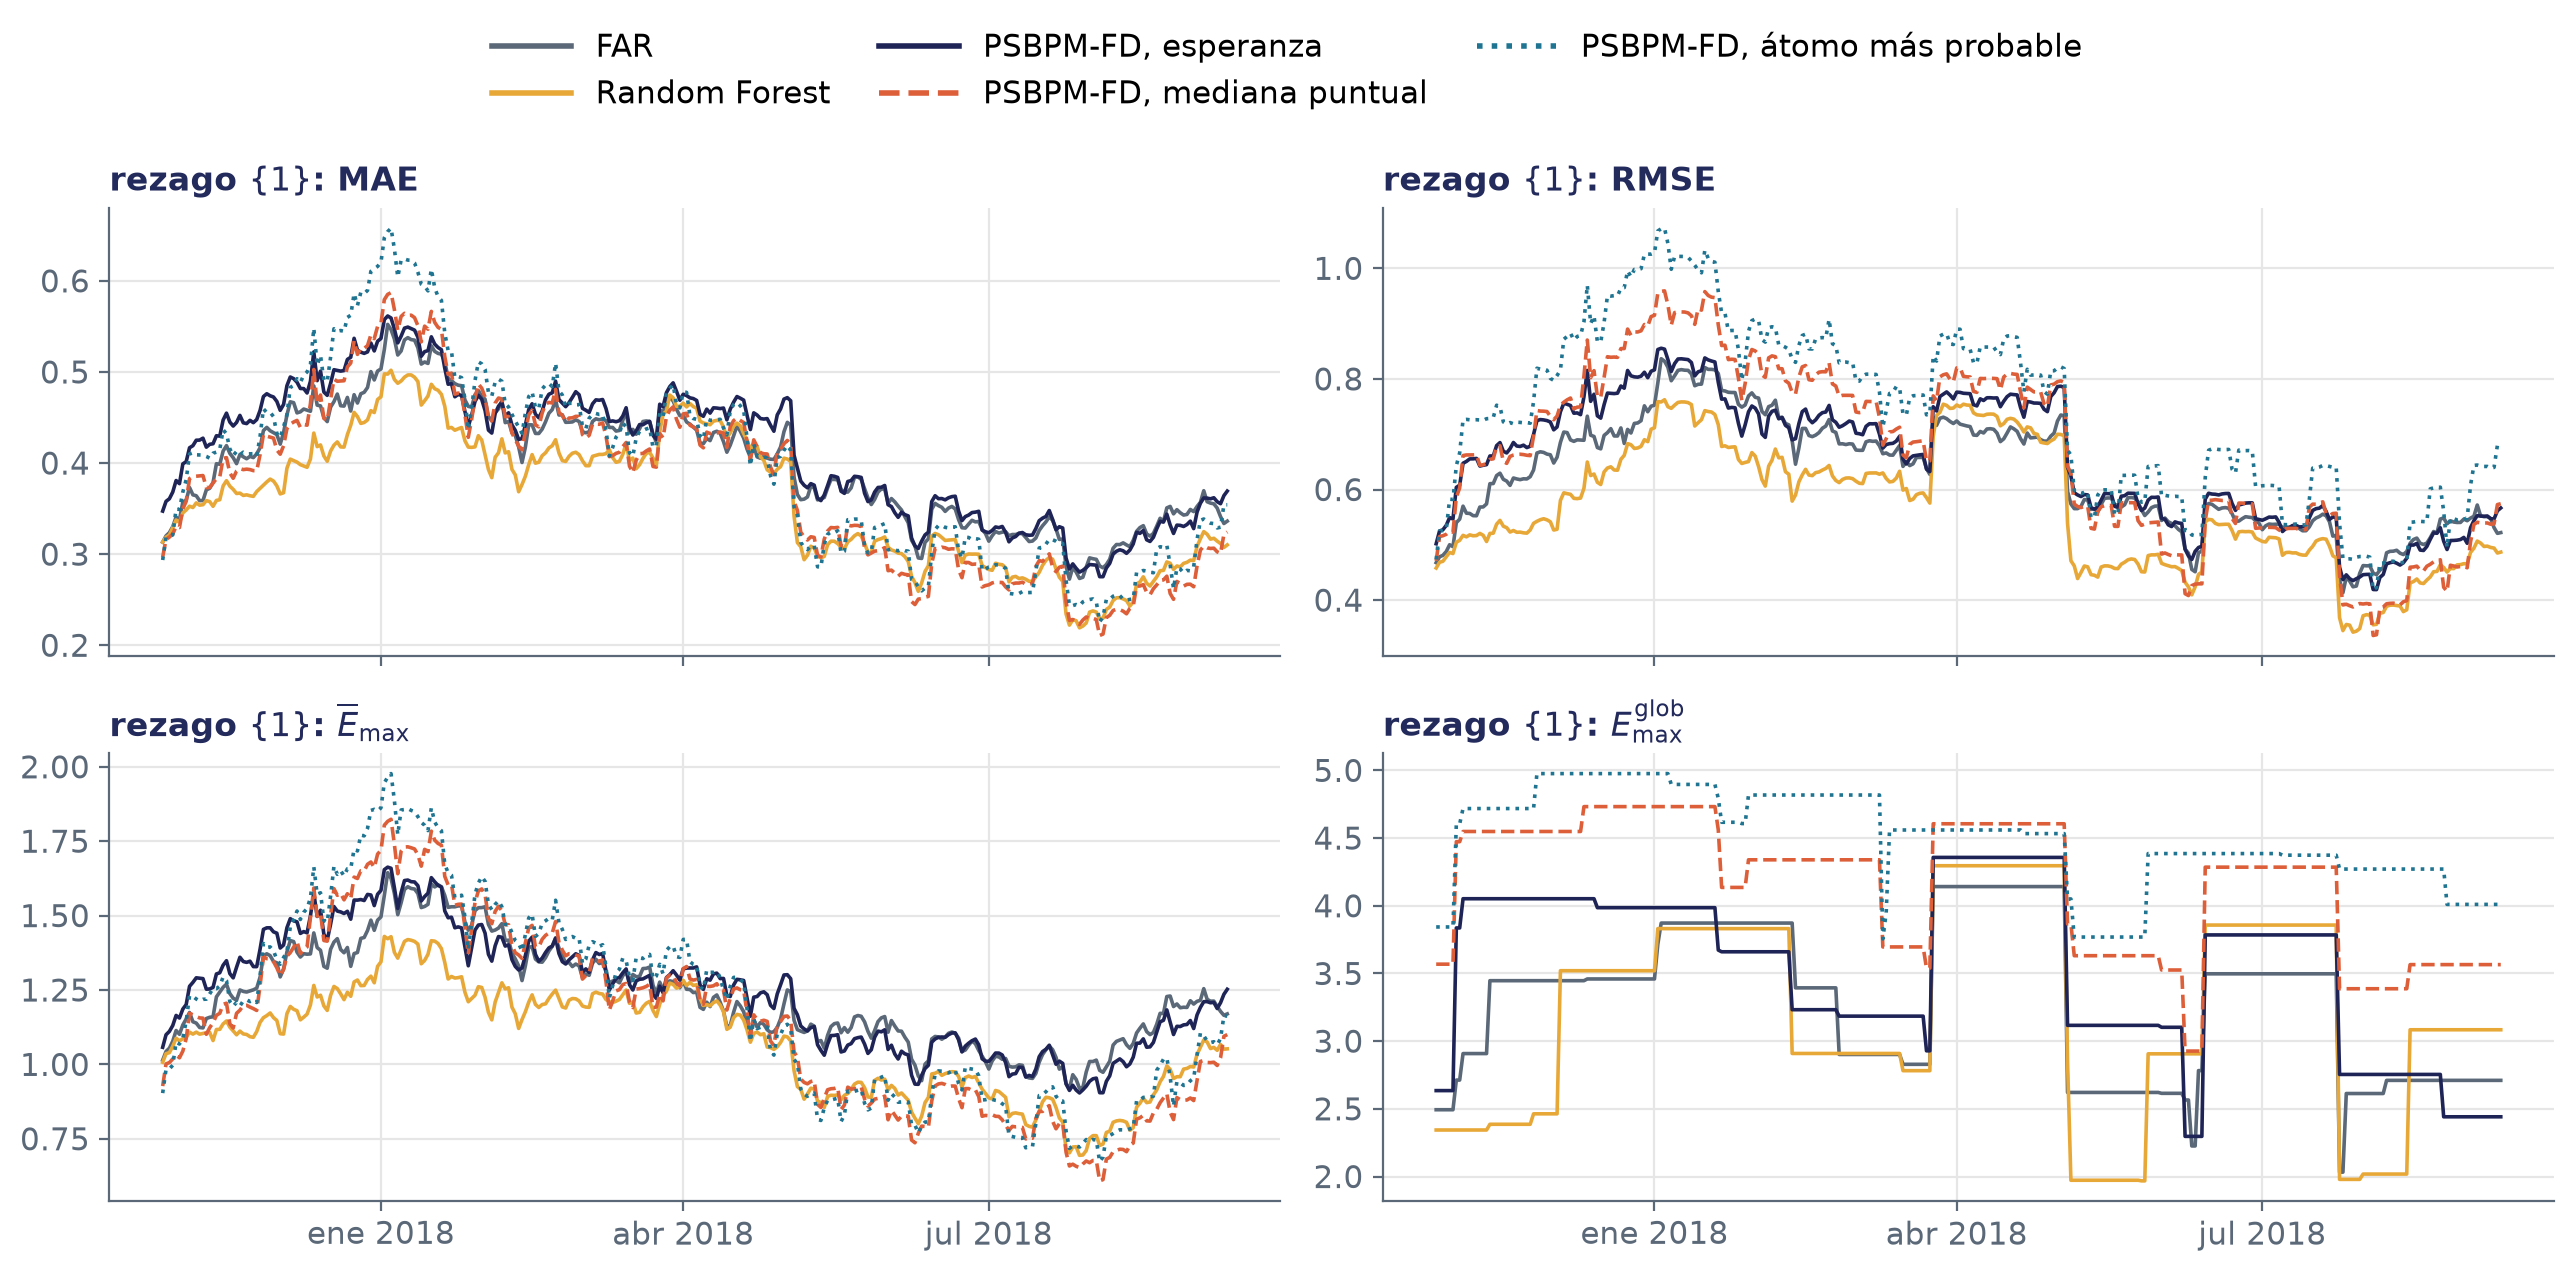
\includegraphics[width=\textwidth]{IMG/aneC_00/aneC_00_58_ventana_predictores_w40_101.png}
\caption{Métricas de error sobre la ventana móvil con $w = 40$, tráfico con rezago $\{1\}$ ($M = 10$).}
\label{fig:aneC_58_ventana_predictores_w40_101}
\end{figure}

\begin{figure}[H]
\centering
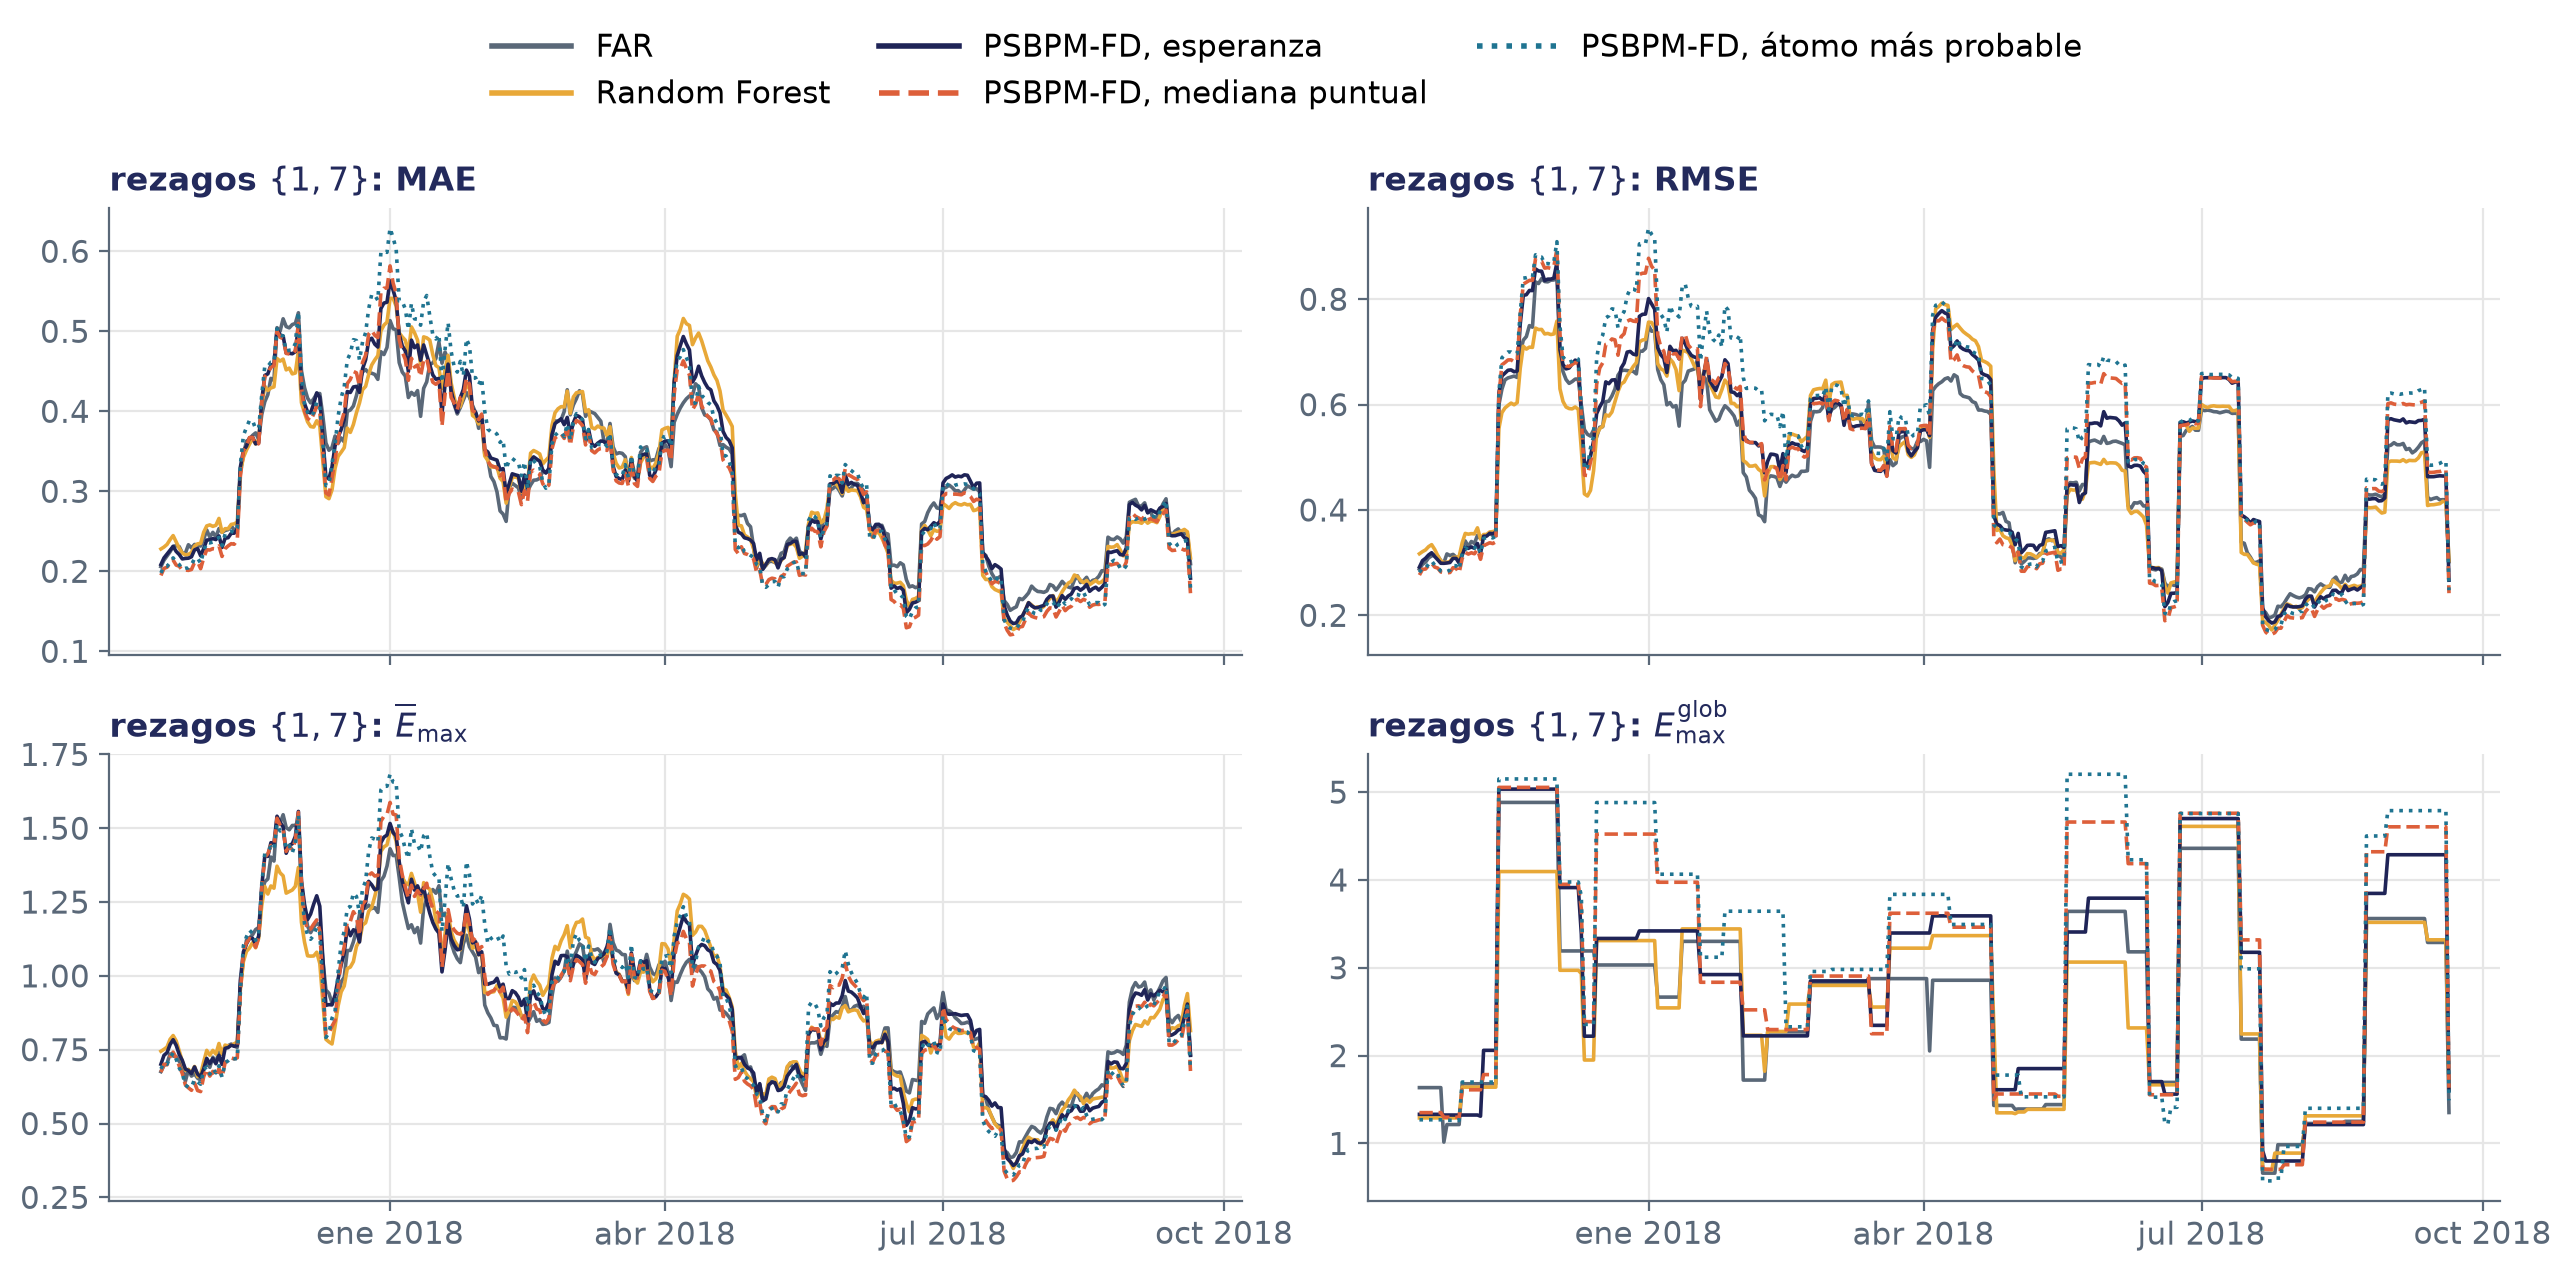
\includegraphics[width=\textwidth]{IMG/aneC_00/aneC_00_58_ventana_predictores_w20_102.png}
\caption{Métricas de error sobre la ventana móvil con $w = 20$, tráfico con rezagos $\{1,7\}$ ($M = 10$).}
\label{fig:aneC_58_ventana_predictores_w20_102}
\end{figure}

\begin{figure}[H]
\centering
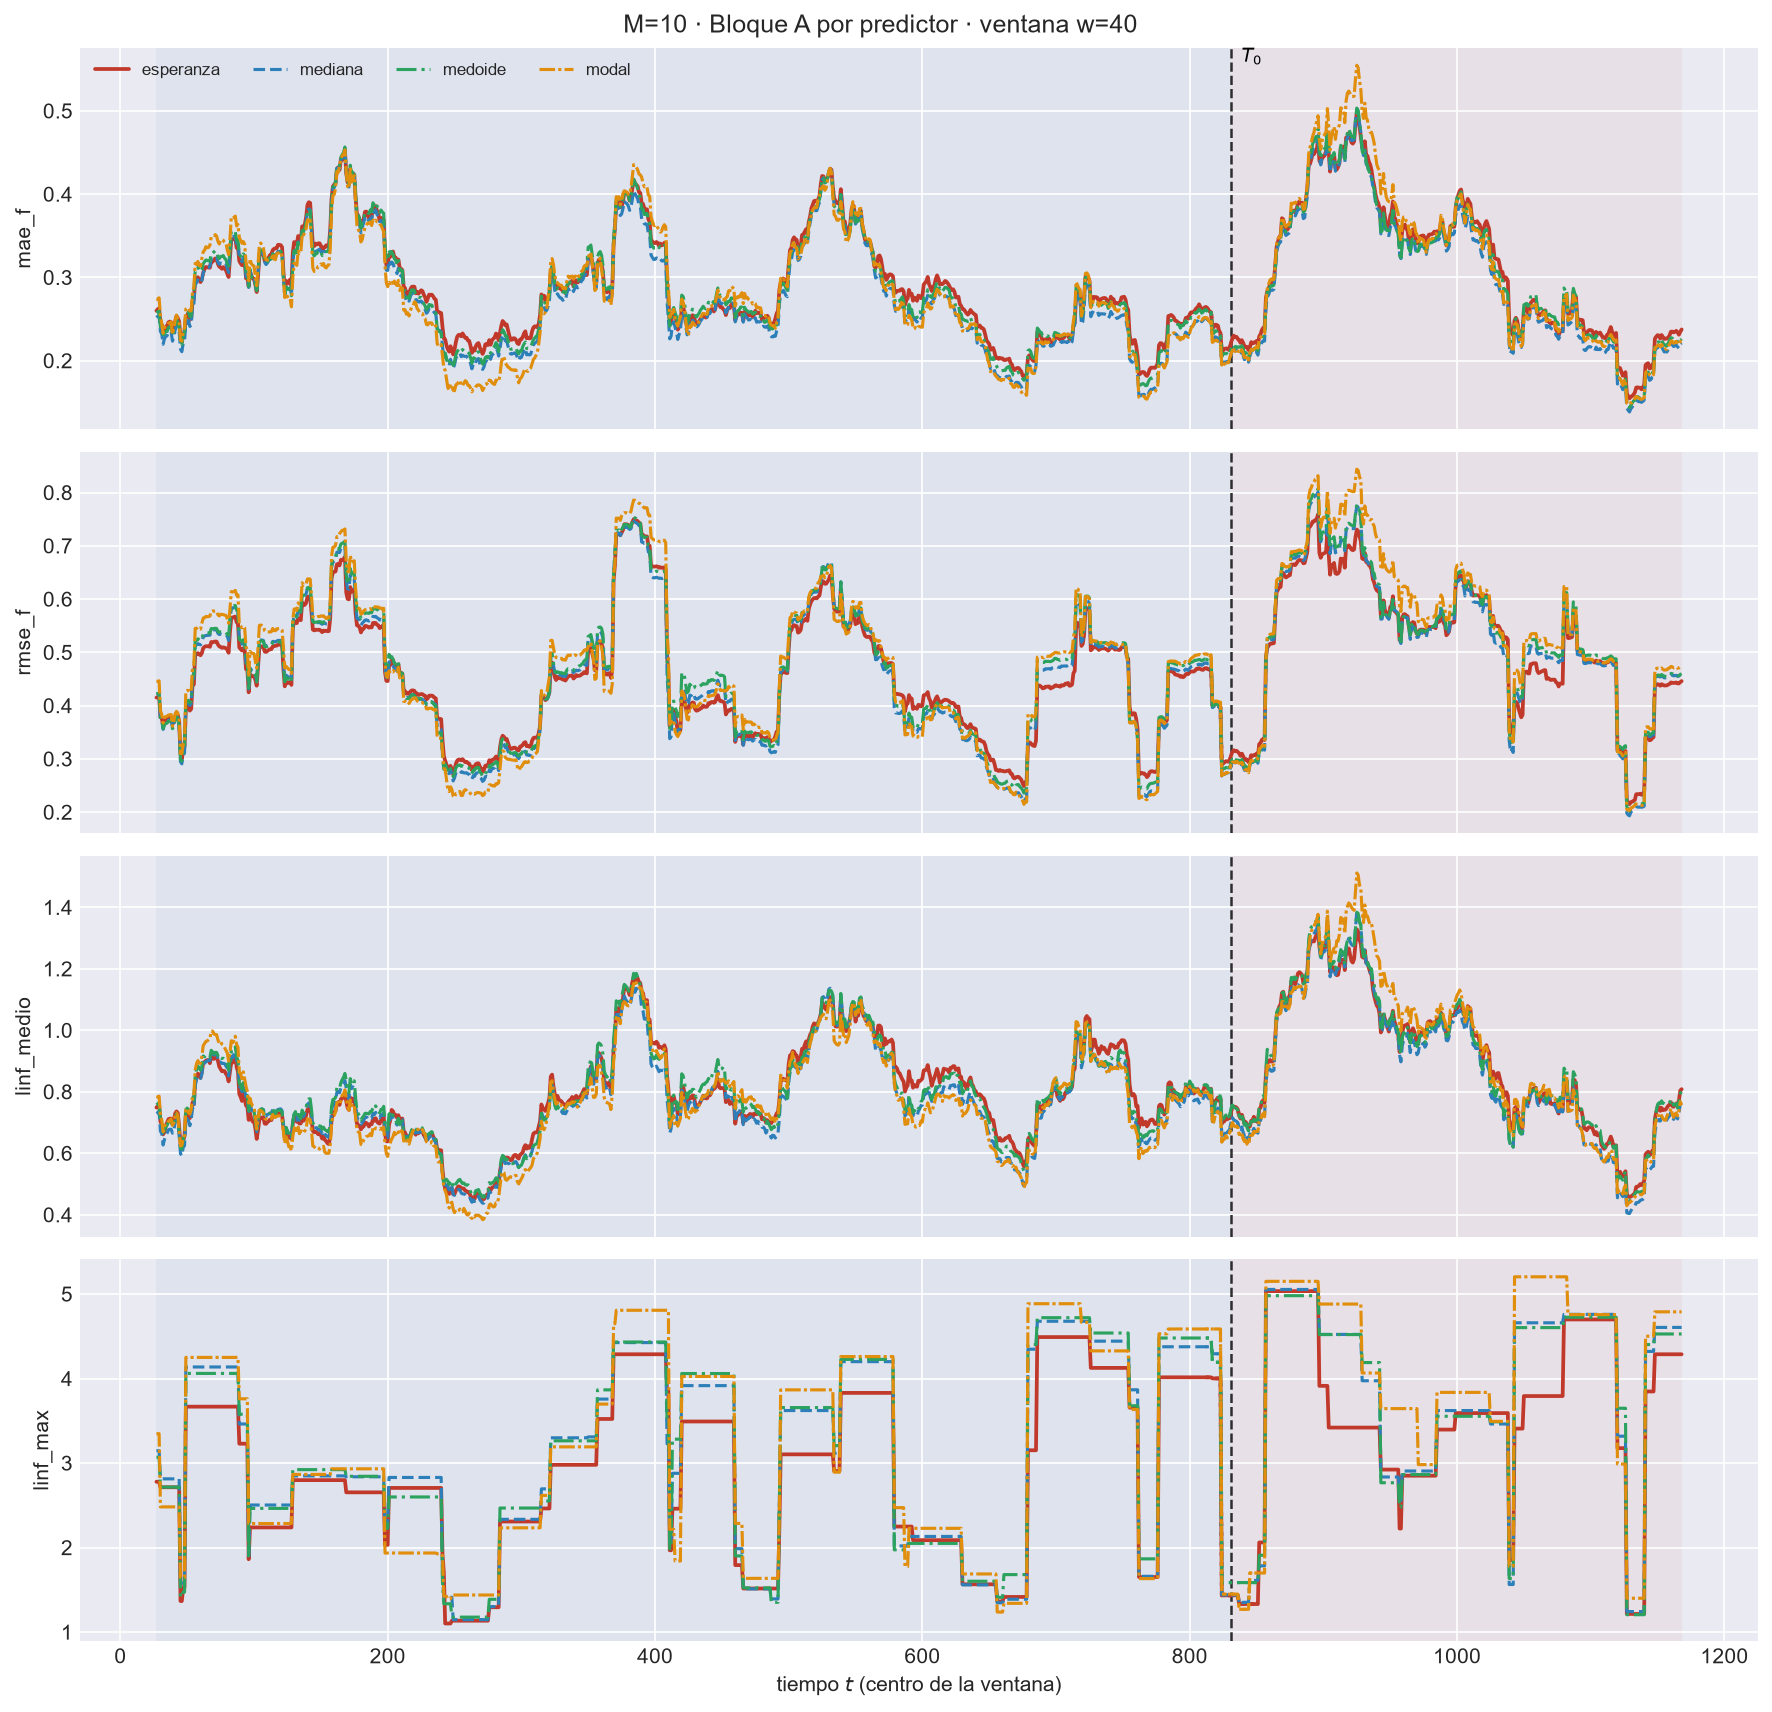
\includegraphics[width=\textwidth]{IMG/aneC_00/aneC_00_58_ventana_predictores_w40_102.png}
\caption{Métricas de error sobre la ventana móvil con $w = 40$, tráfico con rezagos $\{1,7\}$ ($M = 10$).}
\label{fig:aneC_58_ventana_predictores_w40_102}
\end{figure}

\begin{figure}[H]
\centering
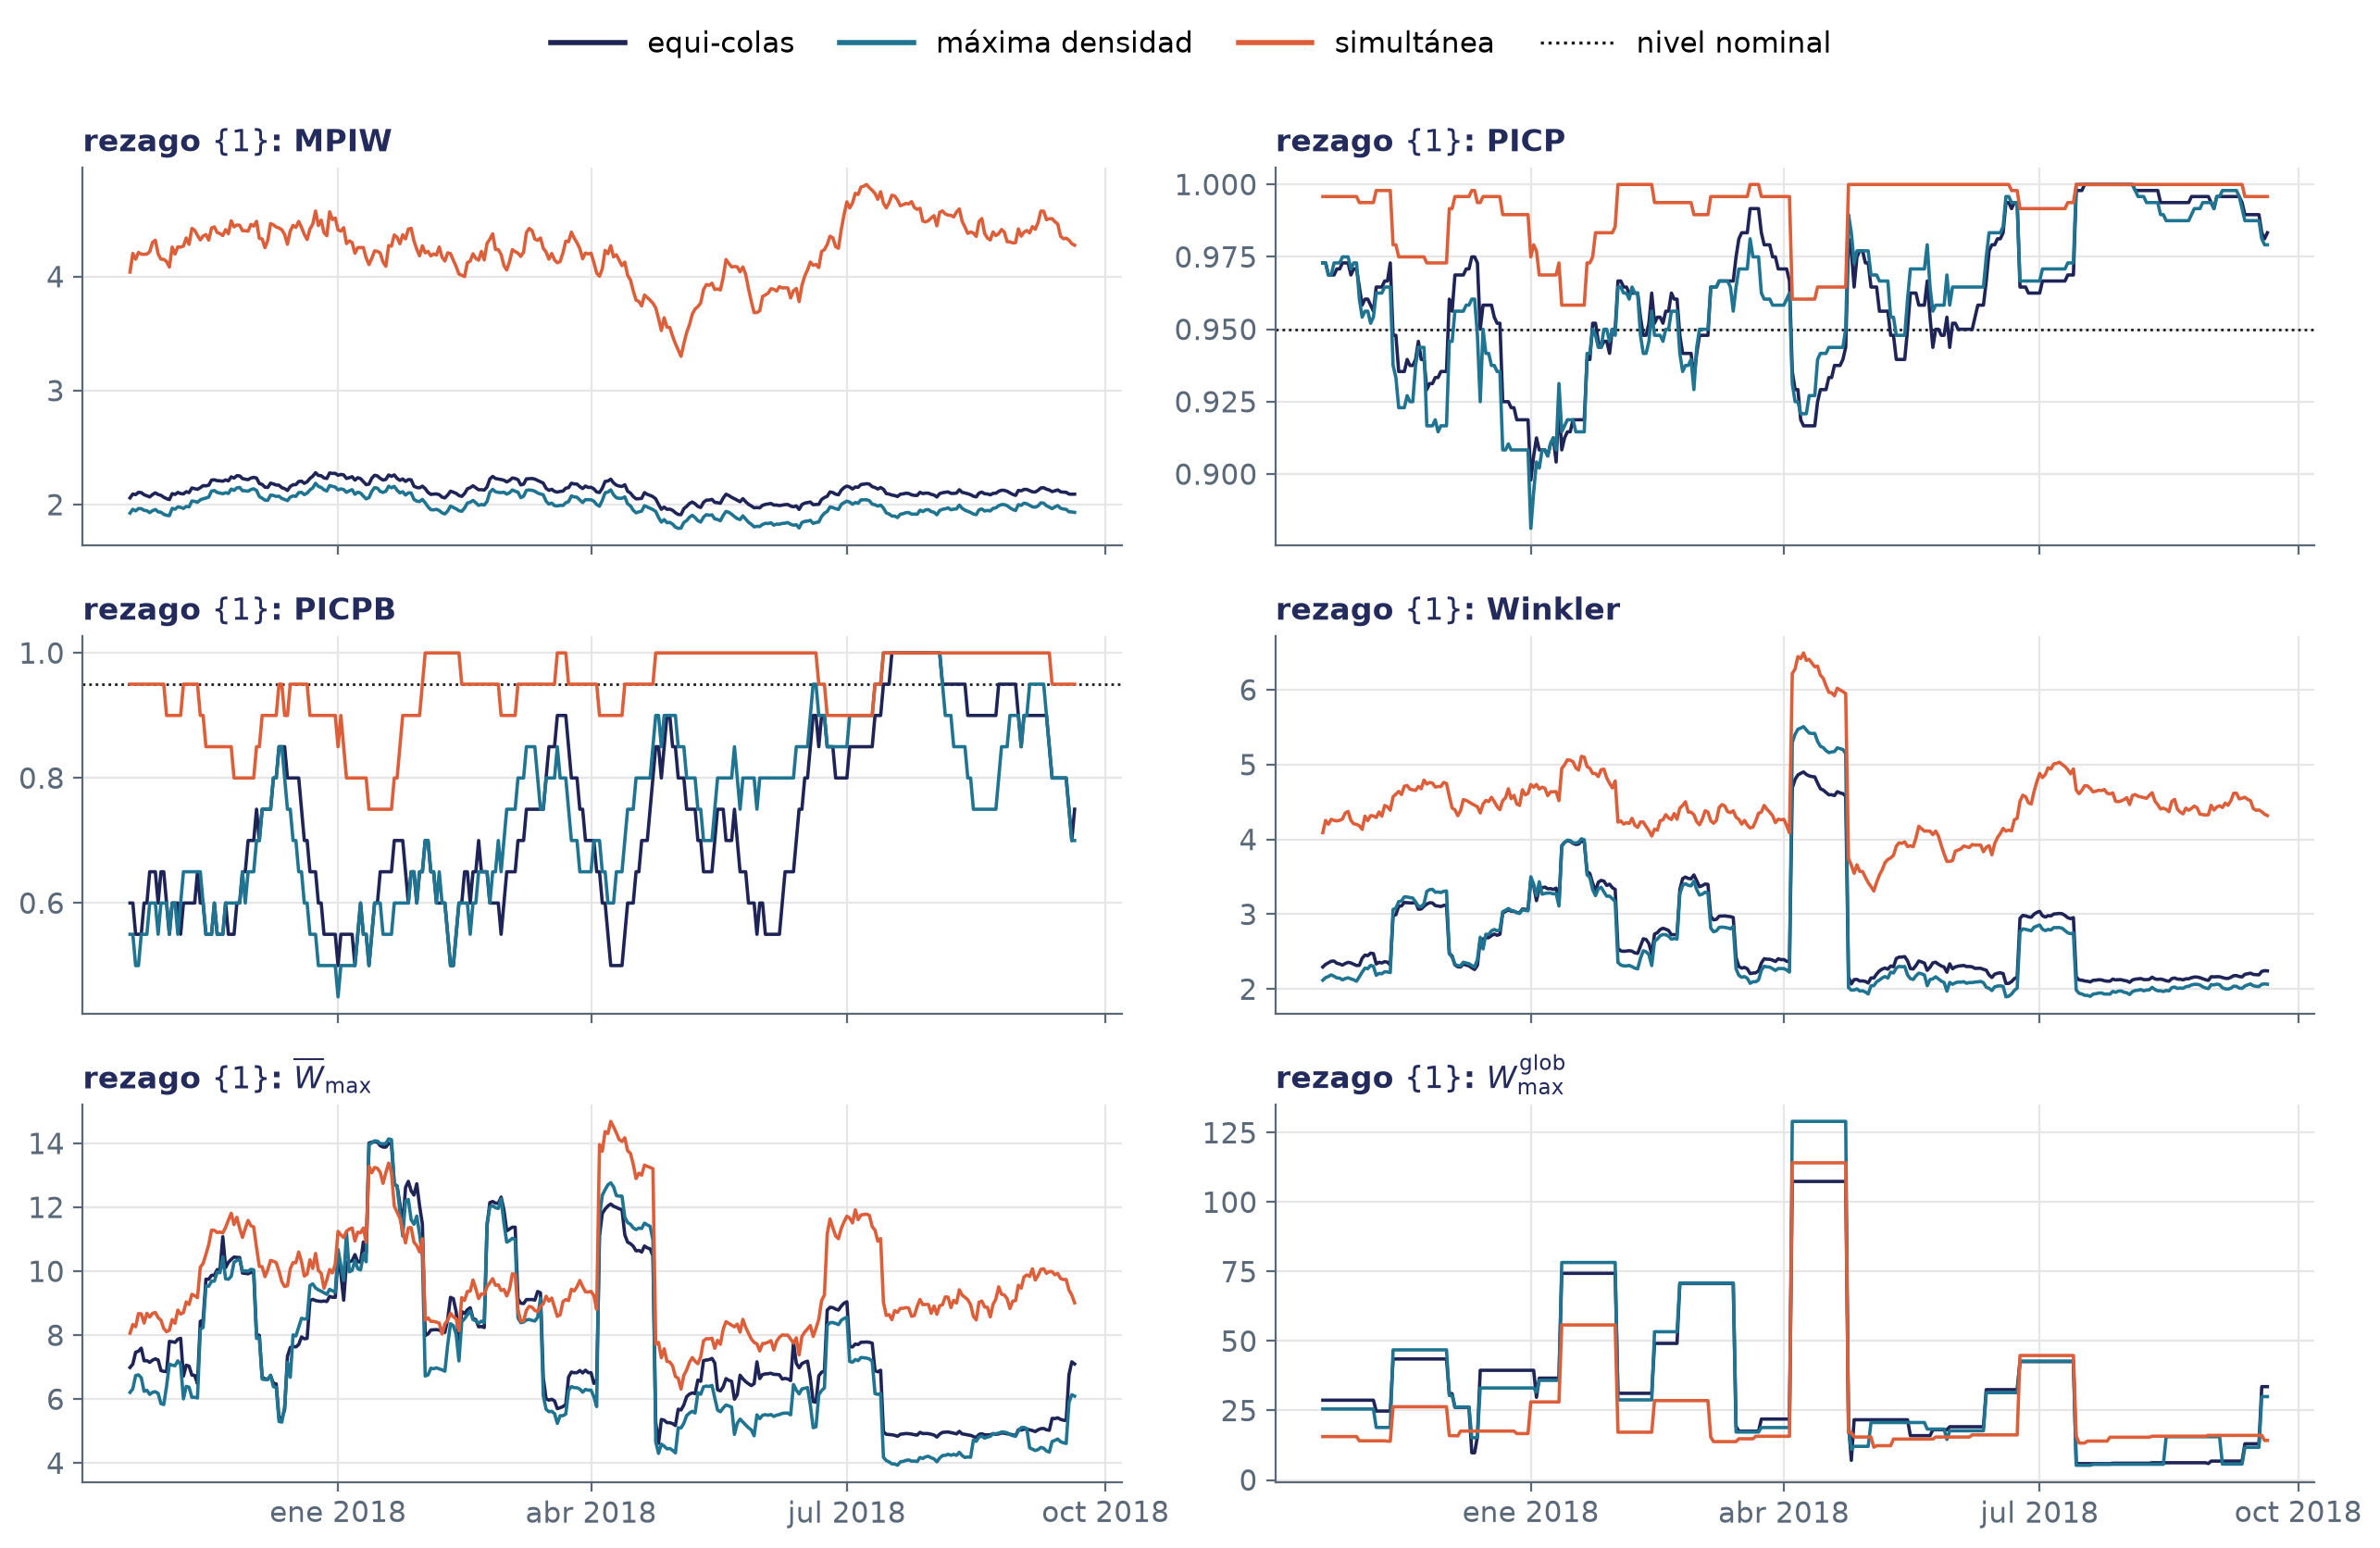
\includegraphics[width=\textwidth]{IMG/aneC_00/aneC_00_59_ventana_intervalos_w20_101.png}
\caption{Métricas de intervalo sobre la ventana móvil con $w = 20$, tráfico con rezago $\{1\}$ ($M = 10$).}
\label{fig:aneC_59_ventana_intervalos_w20_101}
\end{figure}

\begin{figure}[H]
\centering
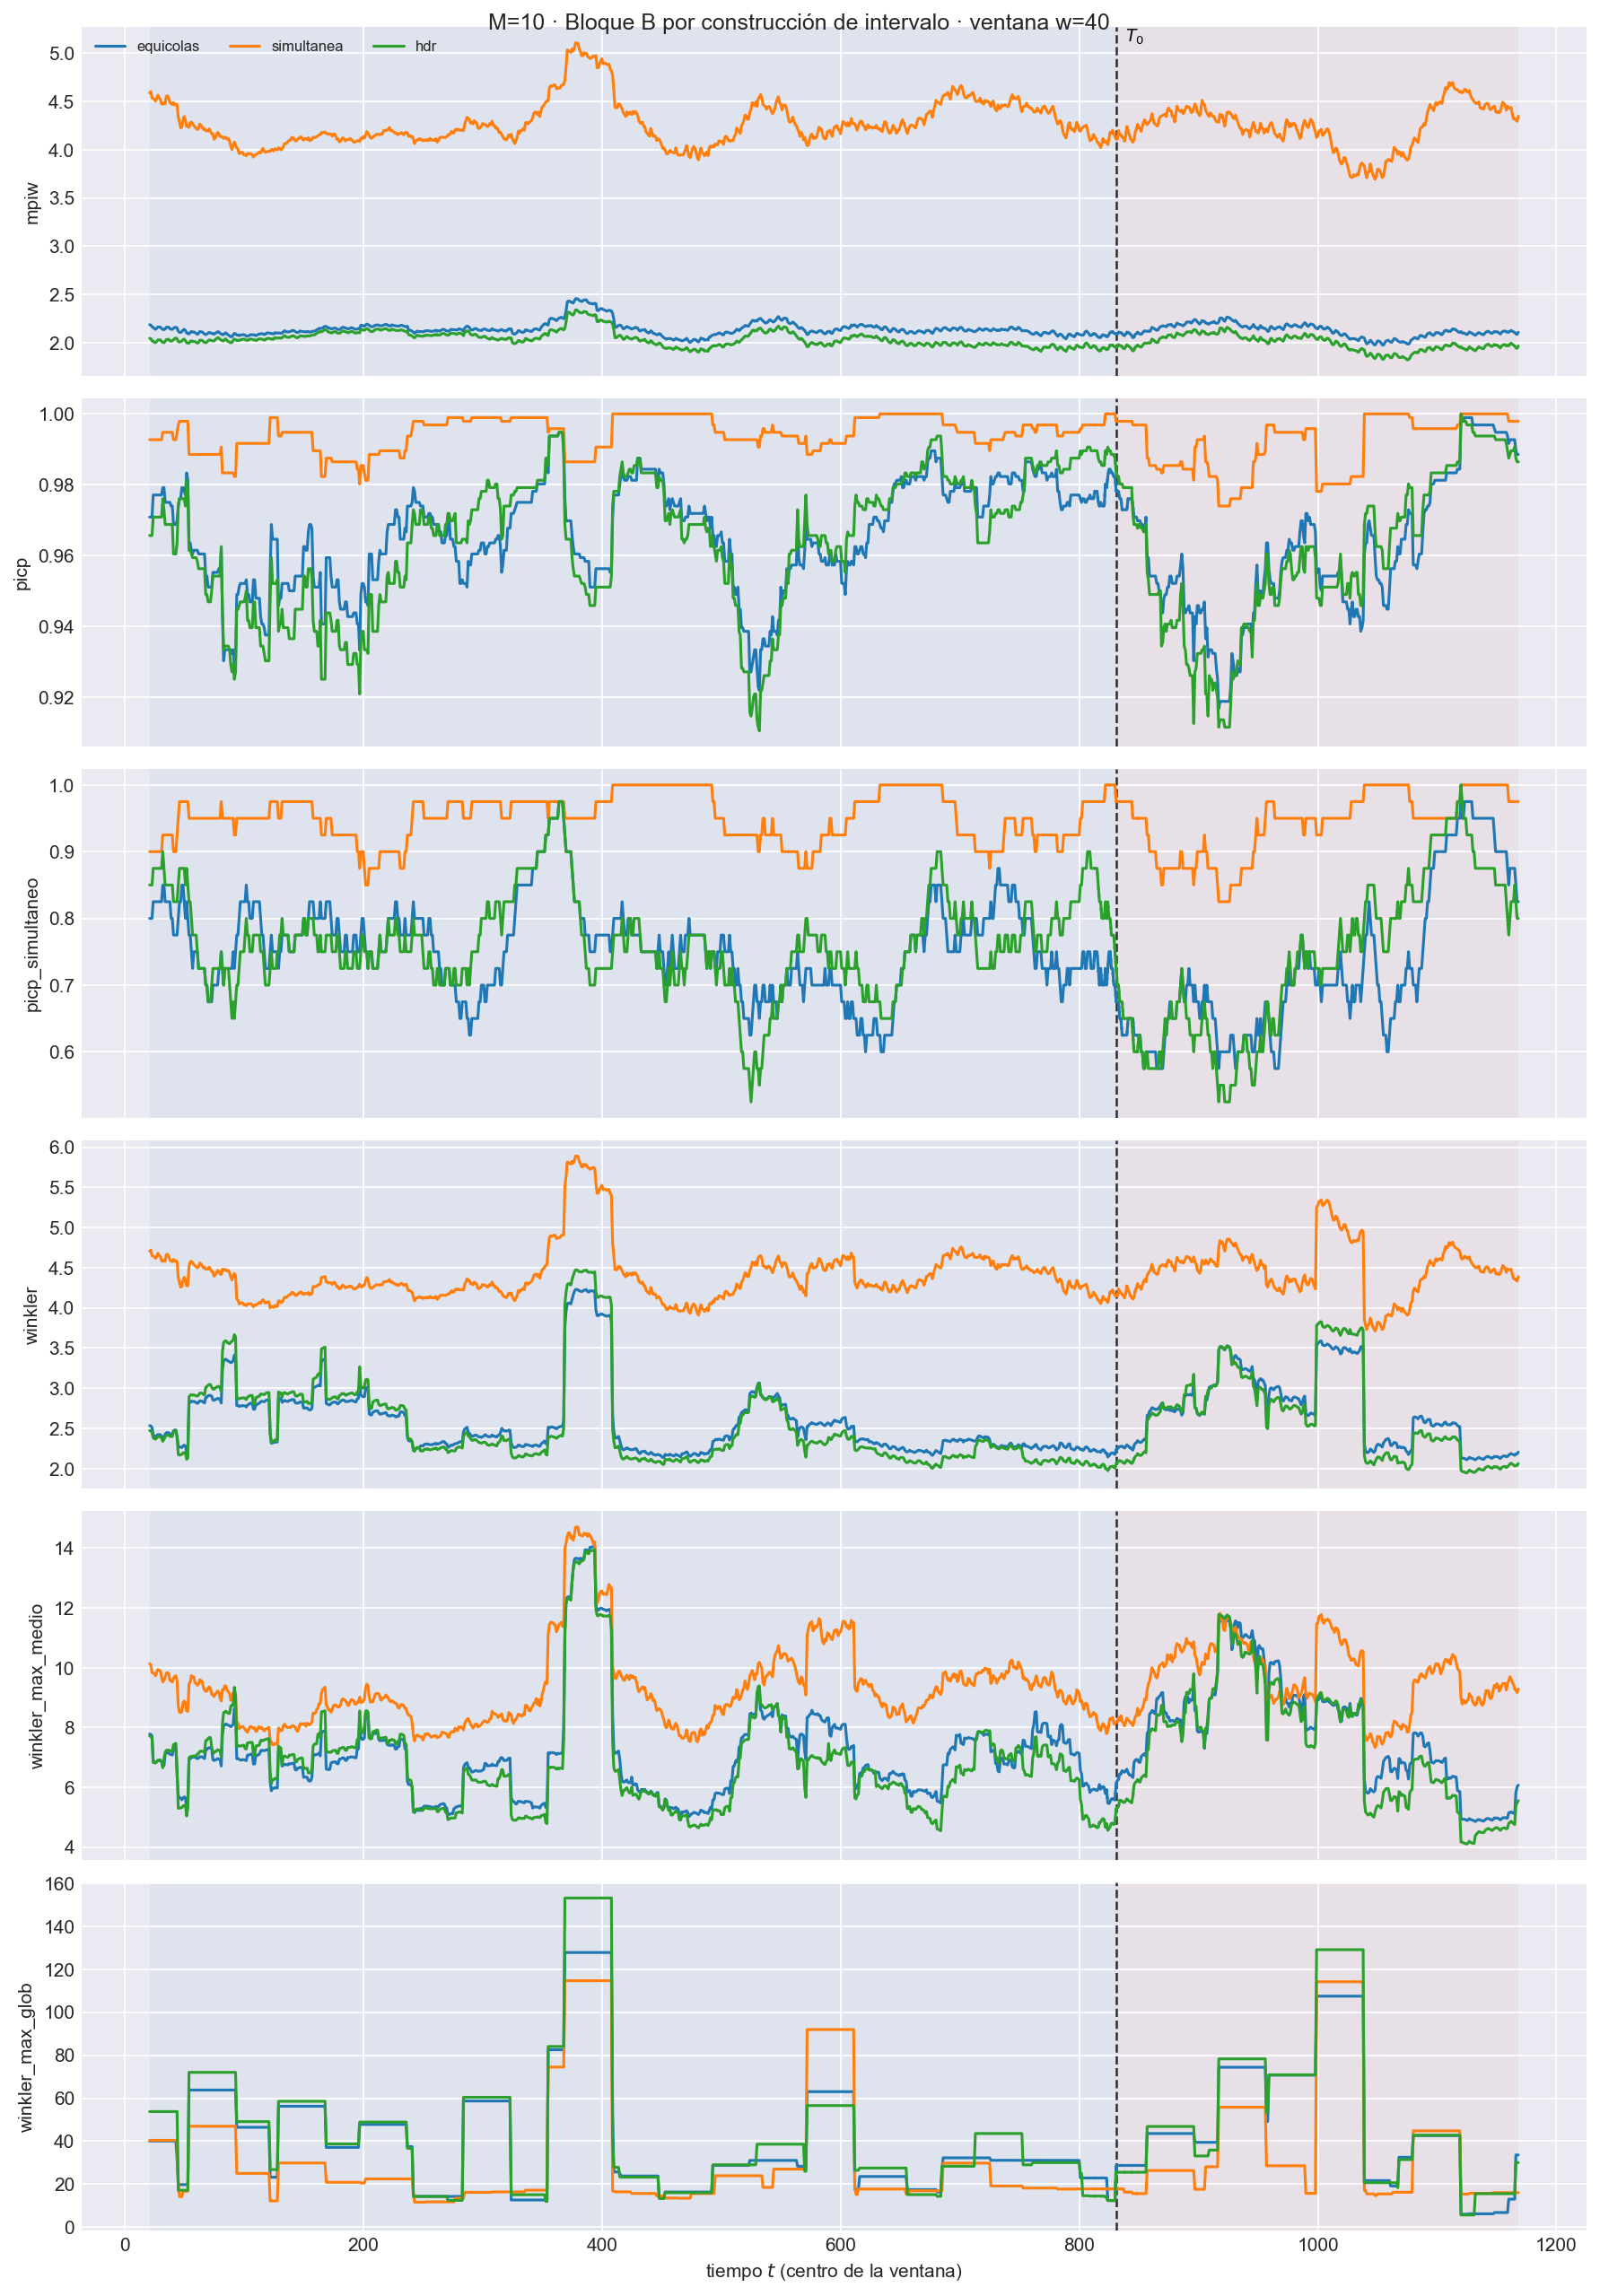
\includegraphics[width=\textwidth]{IMG/aneC_00/aneC_00_59_ventana_intervalos_w40_101.png}
\caption{Métricas de intervalo sobre la ventana móvil con $w = 40$, tráfico con rezago $\{1\}$ ($M = 10$).}
\label{fig:aneC_59_ventana_intervalos_w40_101}
\end{figure}

\begin{figure}[H]
\centering
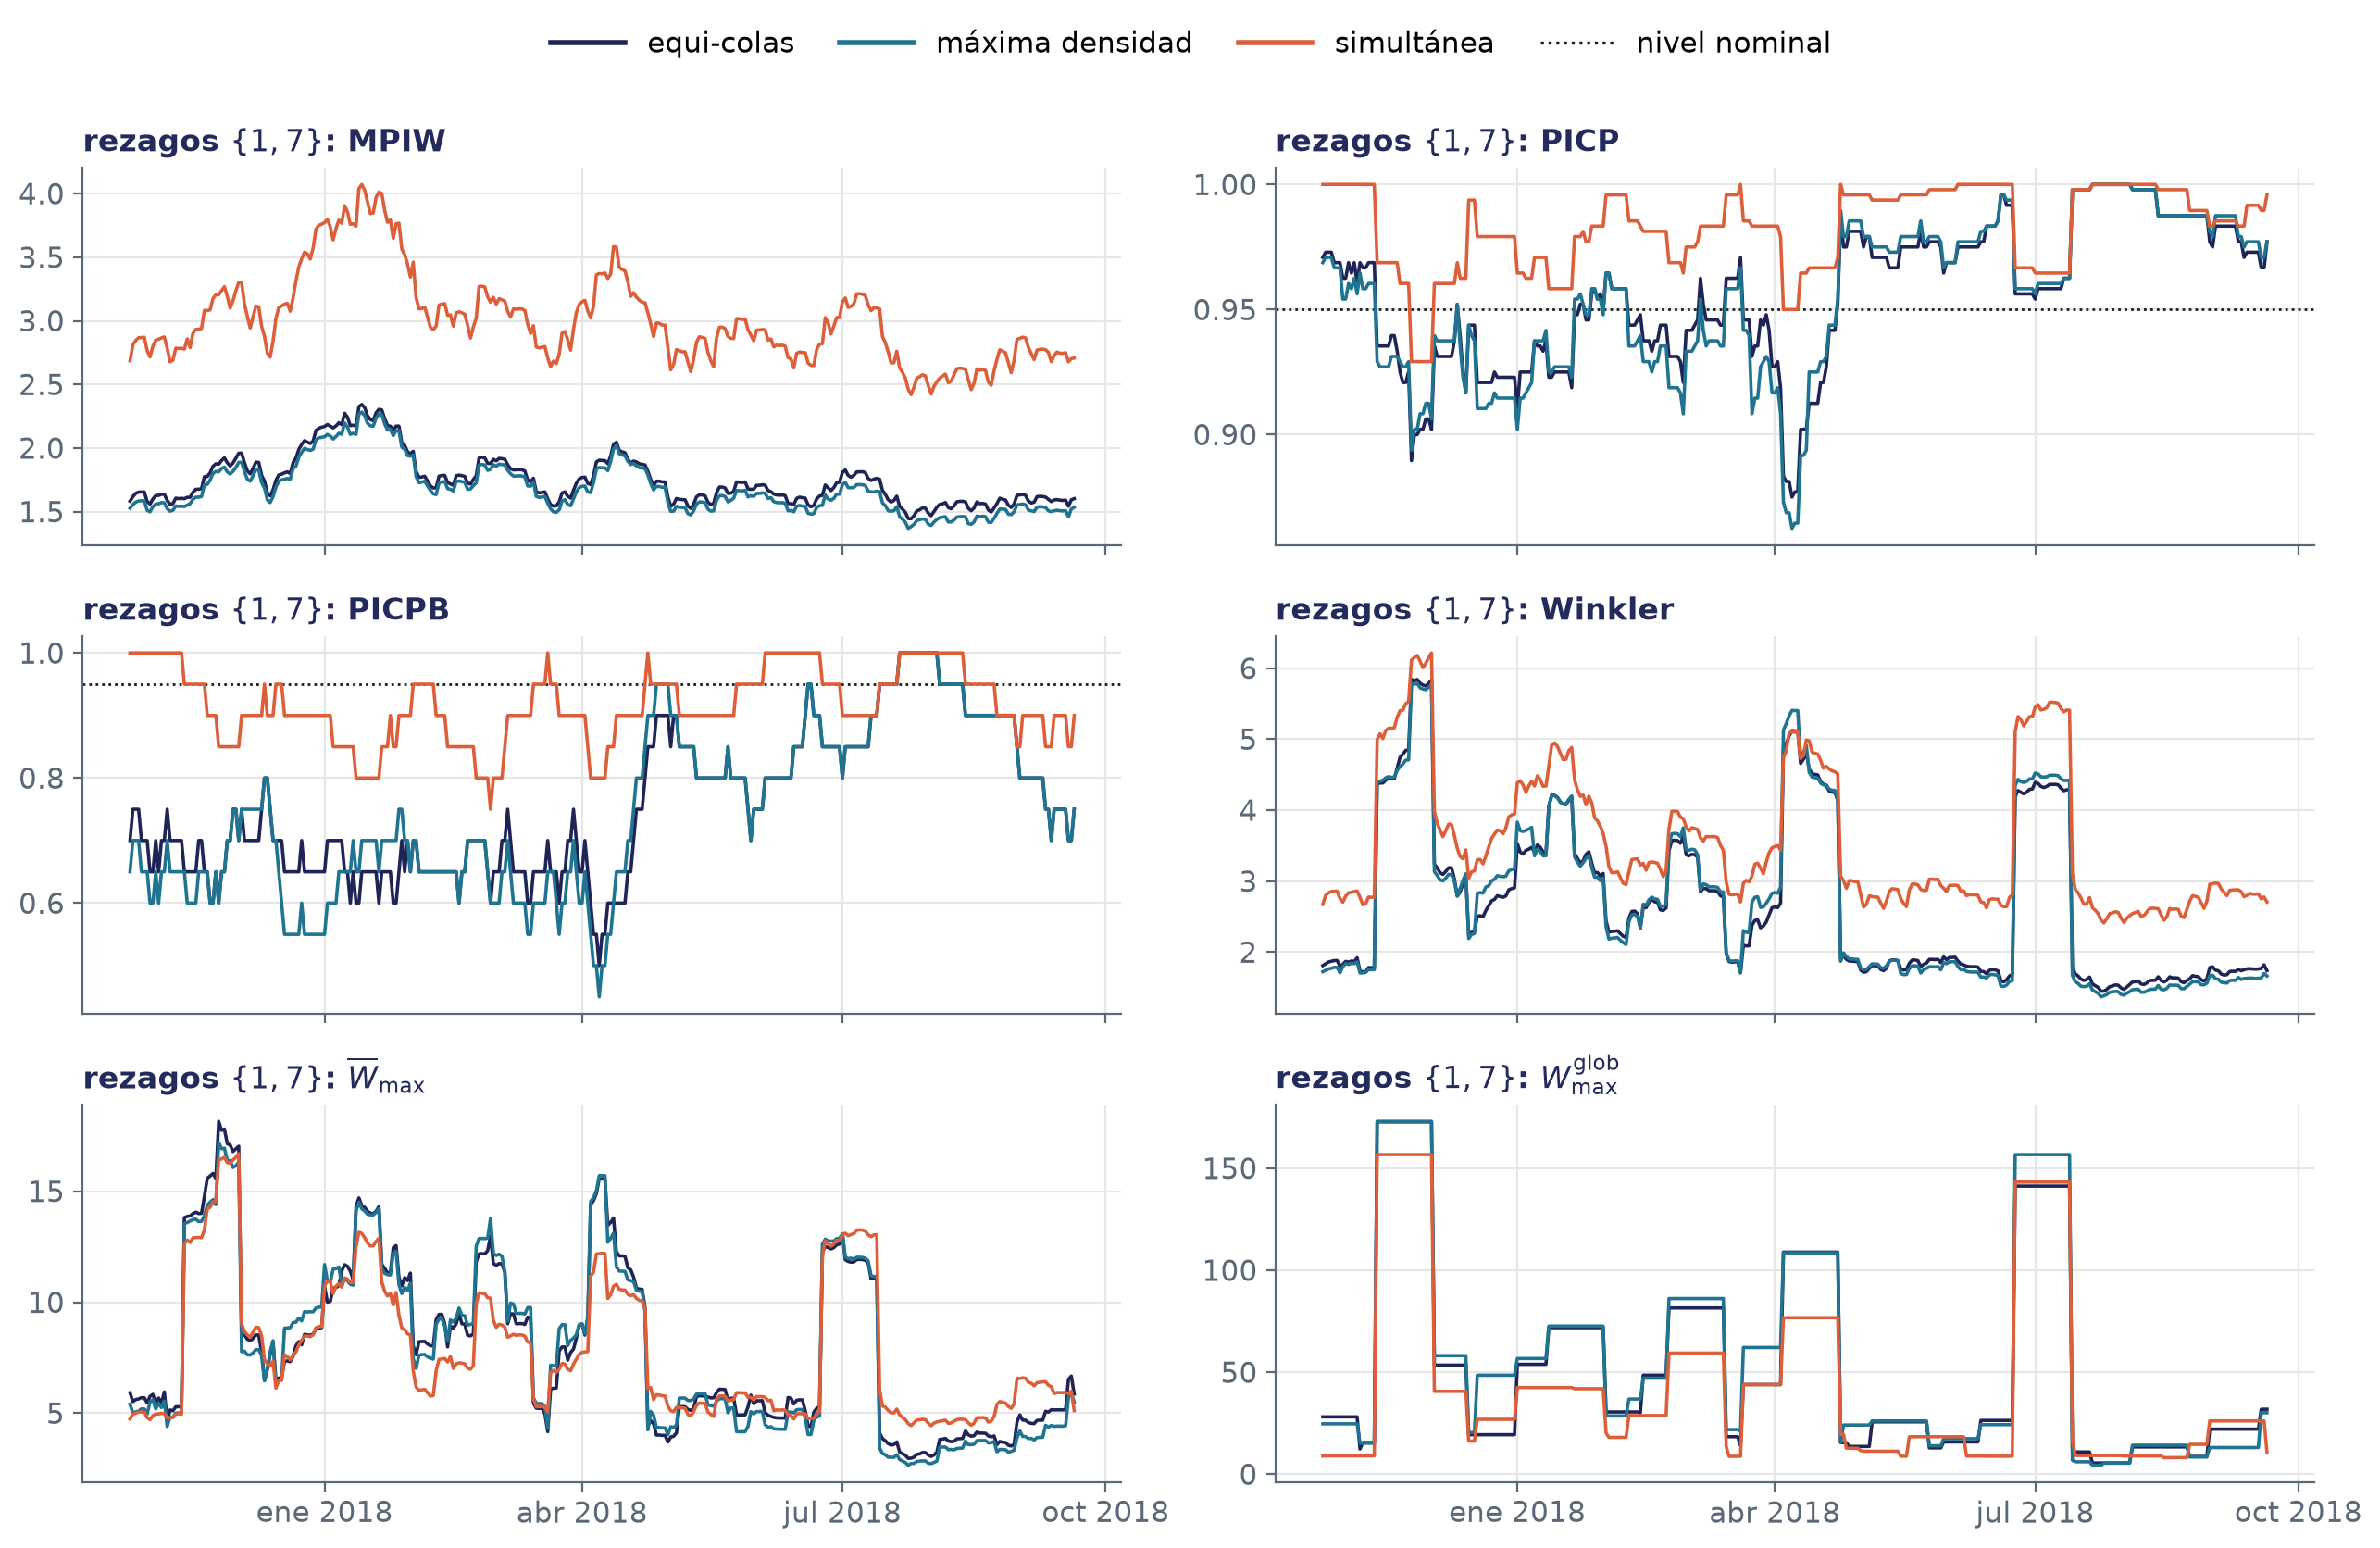
\includegraphics[width=\textwidth]{IMG/aneC_00/aneC_00_59_ventana_intervalos_w20_102.png}
\caption{Métricas de intervalo sobre la ventana móvil con $w = 20$, tráfico con rezagos $\{1,7\}$ ($M = 10$).}
\label{fig:aneC_59_ventana_intervalos_w20_102}
\end{figure}

\begin{figure}[H]
\centering
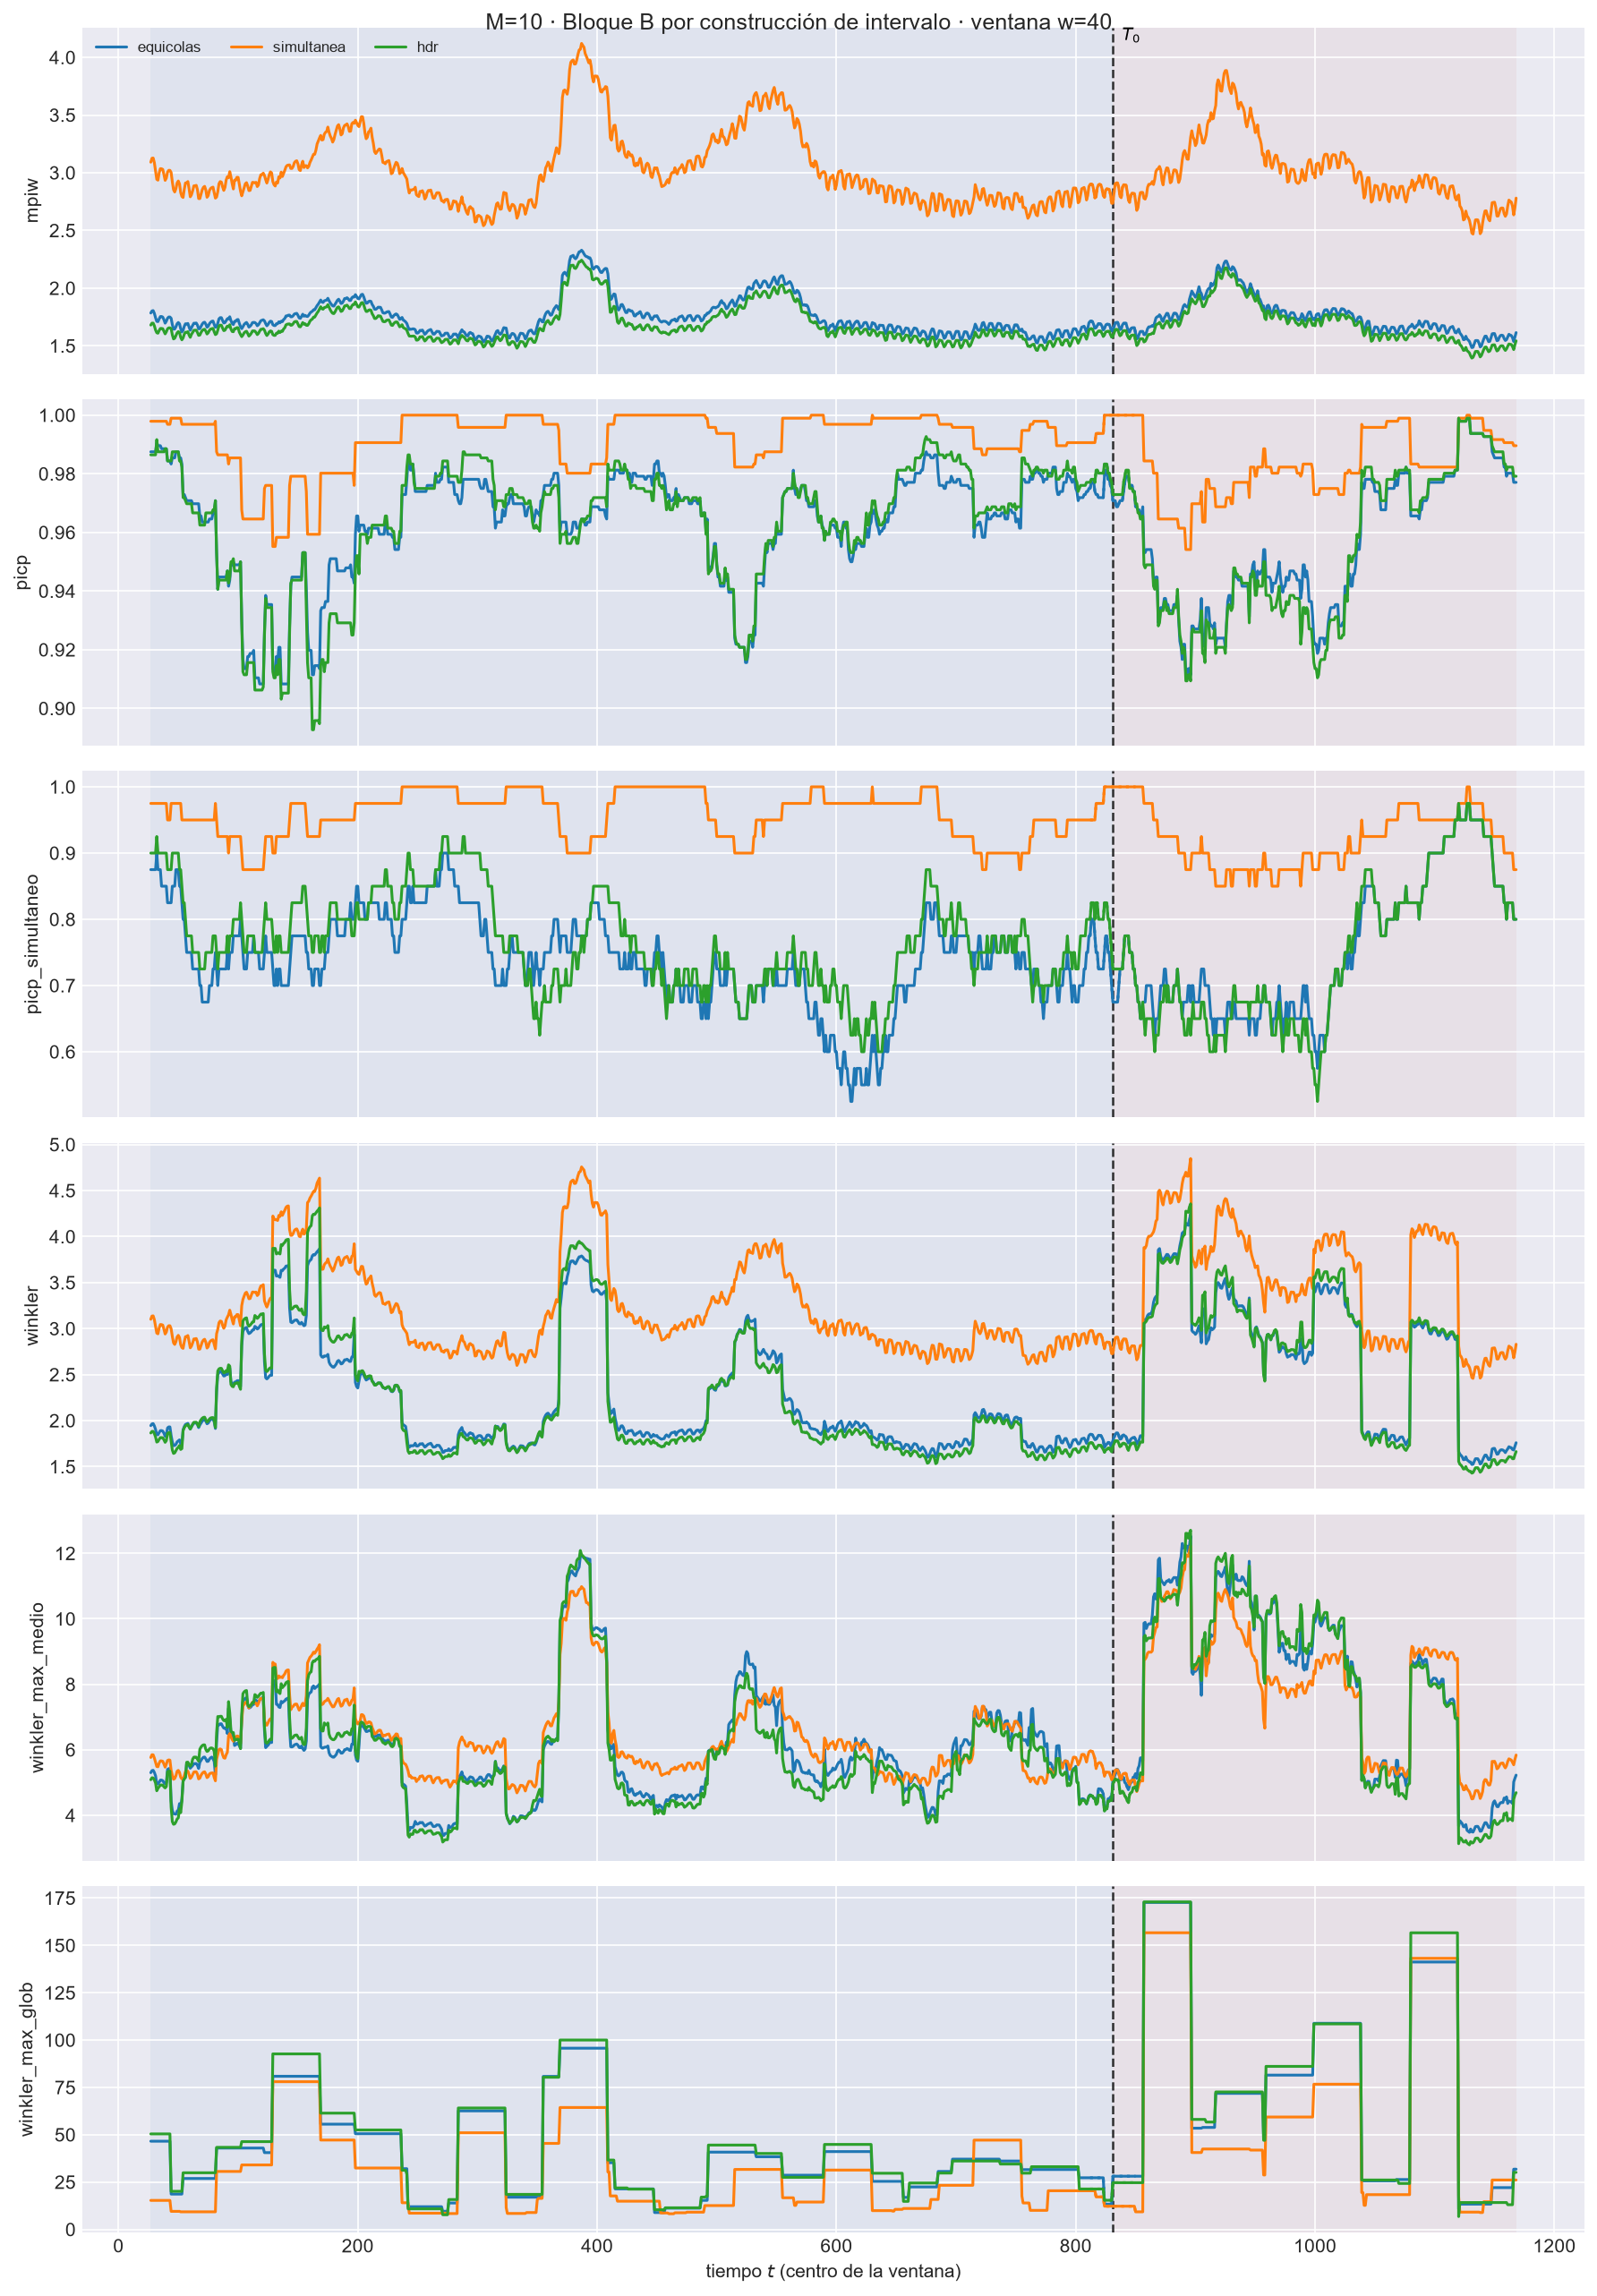
\includegraphics[width=\textwidth]{IMG/aneC_00/aneC_00_59_ventana_intervalos_w40_102.png}
\caption{Métricas de intervalo sobre la ventana móvil con $w = 40$, tráfico con rezagos $\{1,7\}$ ($M = 10$).}
\label{fig:aneC_59_ventana_intervalos_w40_102}
\end{figure}

\section{Predicciones curva a curva}
\label{aneC_00_05_curvas}
% 54 y 55: extractos del bloque de prueba y de la frontera; 56b: el peor origen por RMSE; 61b: predictores.

Extractos de predicciones del bloque de prueba, la ventana de peor RMSE y los tres predictores puntuales en cuatro orígenes de la ventana de detalle.

\begin{figure}[H]
\centering
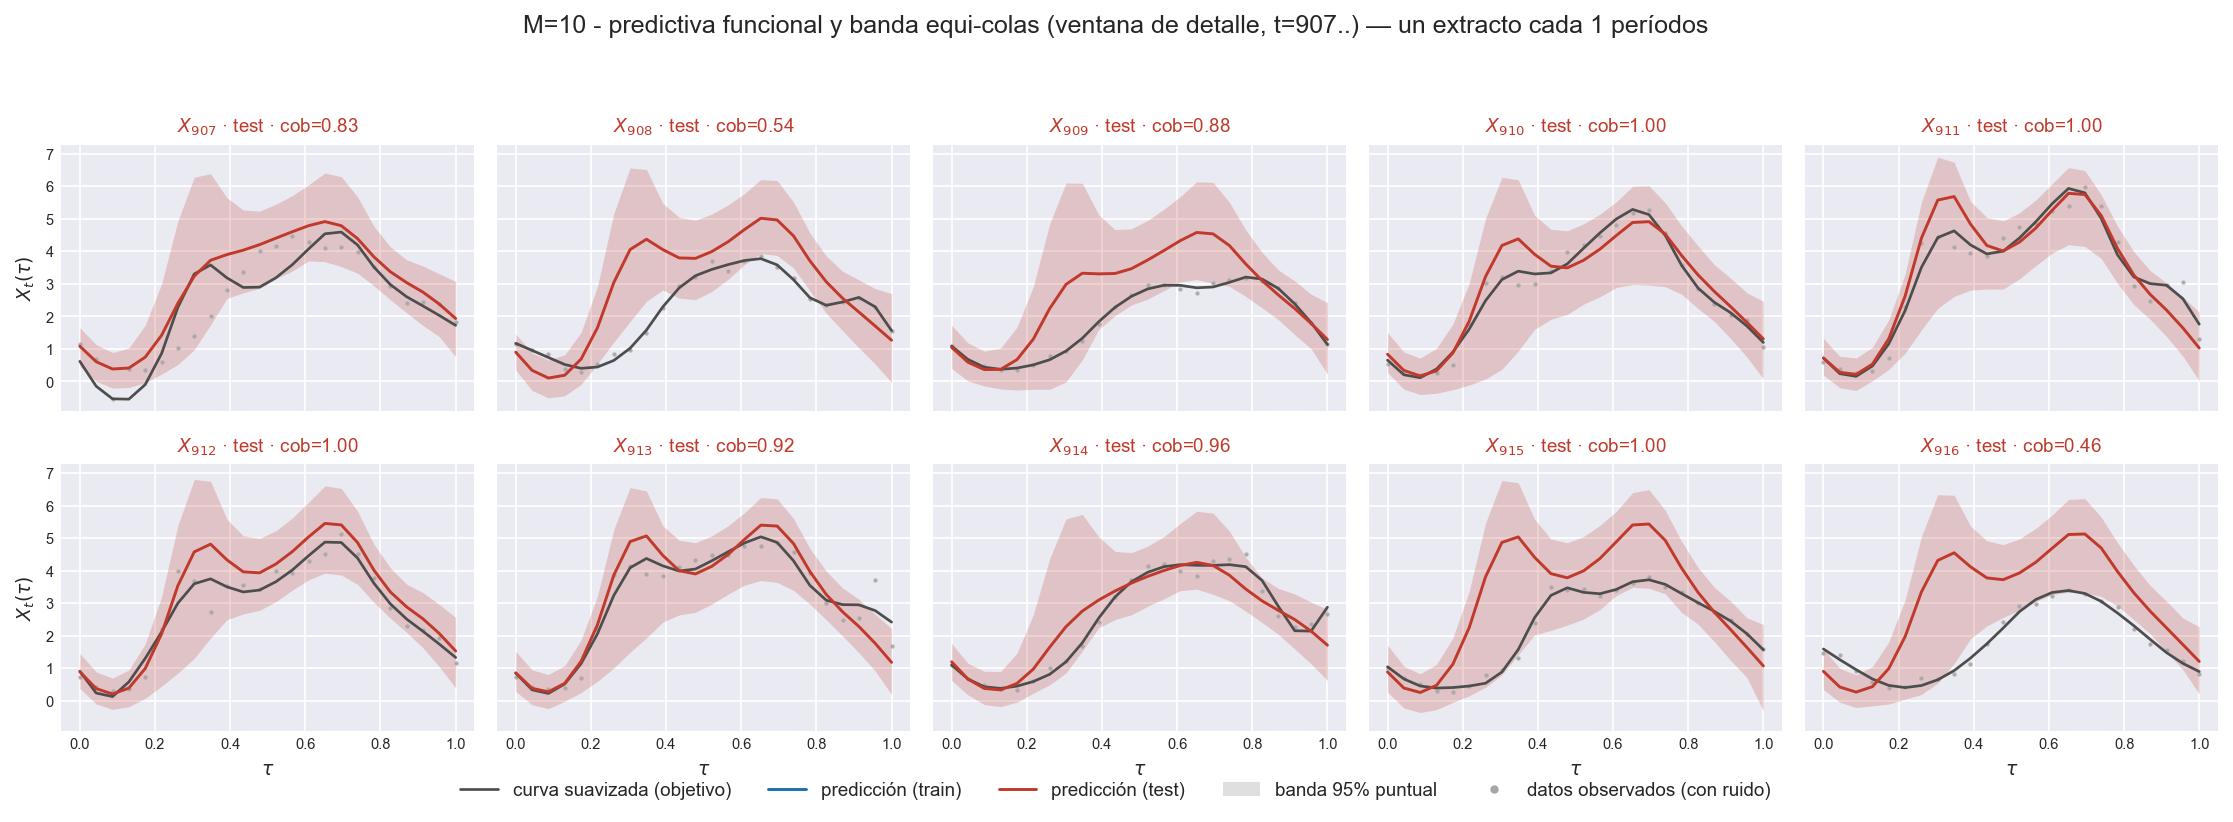
\includegraphics[width=\textwidth,height=0.8\textheight,keepaspectratio]{IMG/aneC_00/aneC_00_54_extractos_curvas_test_101.png}
\caption{Extractos de predicciones del bloque de prueba, tráfico con rezago $\{1\}$ ($M = 10$).}
\label{fig:aneC_54_extractos_curvas_test_101}
\end{figure}

\begin{figure}[H]
\centering
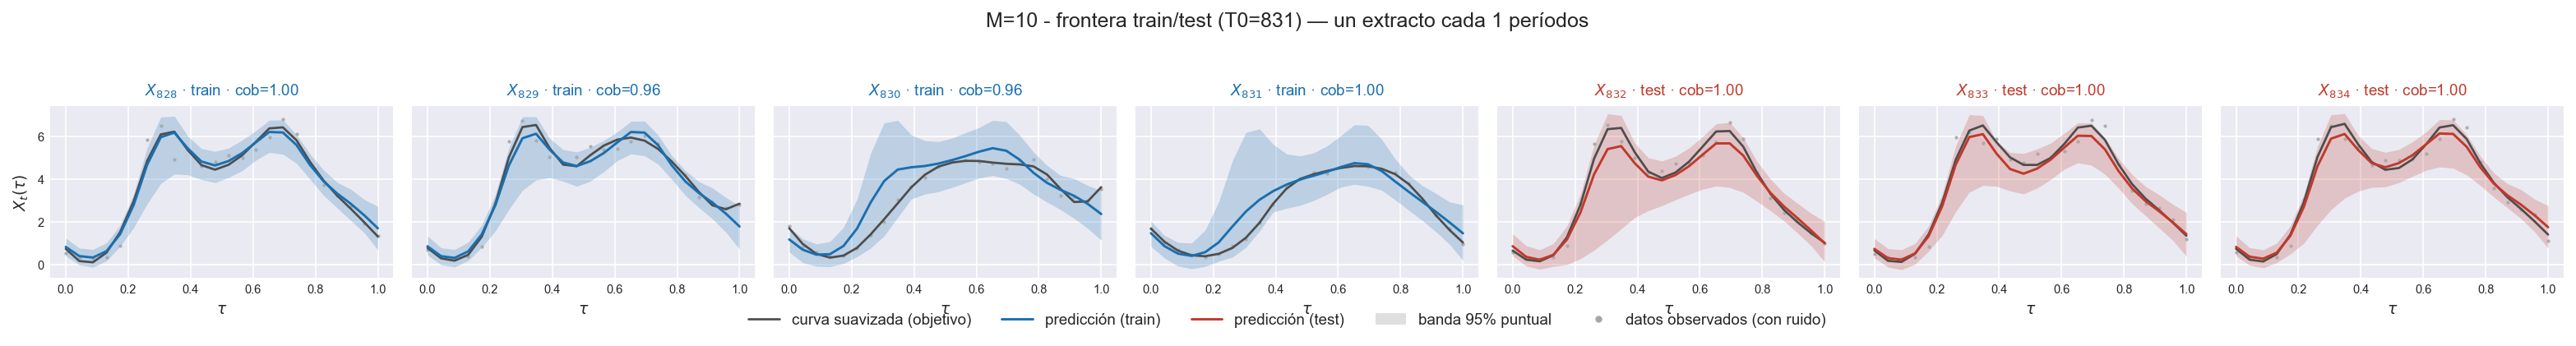
\includegraphics[width=\textwidth,height=0.8\textheight,keepaspectratio]{IMG/aneC_00/aneC_00_55_extractos_frontera_101.png}
\caption{Predicciones en la frontera entre los bloques de entrenamiento y de prueba, tráfico con rezago $\{1\}$ ($M = 10$).}
\label{fig:aneC_55_extractos_frontera_101}
\end{figure}

\begin{figure}[H]
\centering
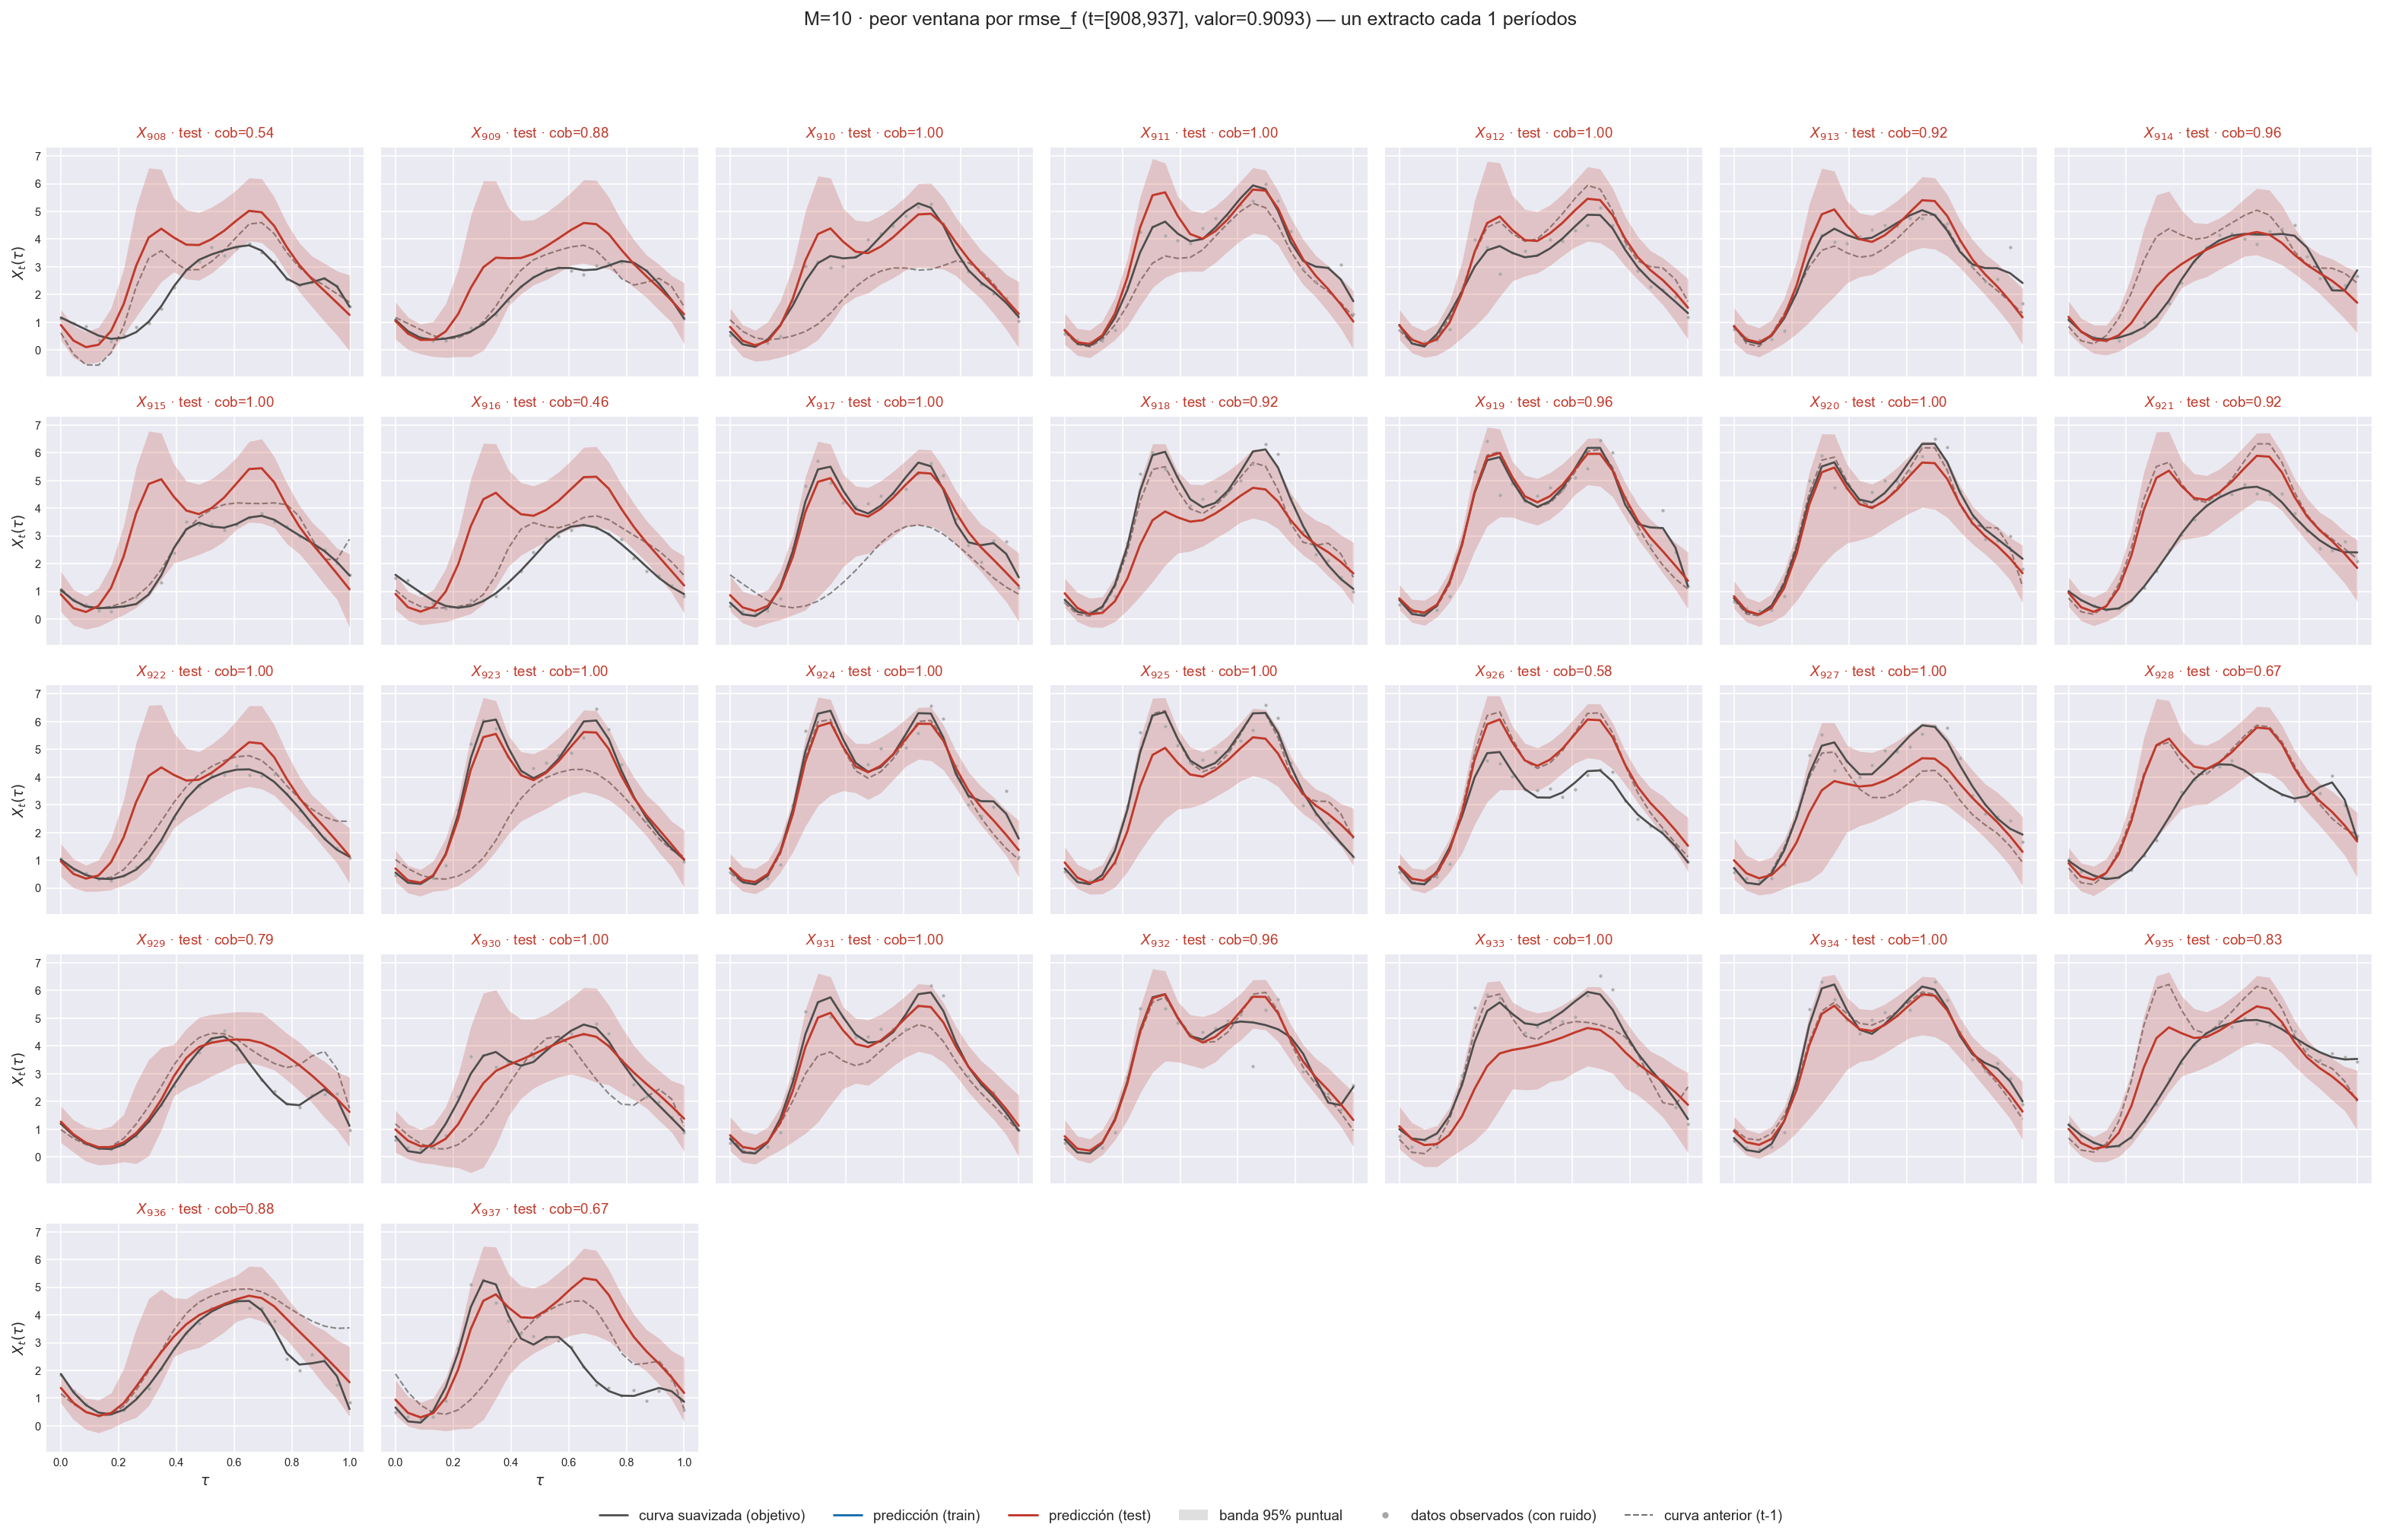
\includegraphics[width=\textwidth,height=0.8\textheight,keepaspectratio]{IMG/aneC_00/aneC_00_56b_peor_ventana_rmse_f_t908_101.png}
\caption{Ventana de peor RMSE (origen $t = 908$), tráfico con rezago $\{1\}$ ($M = 10$).}
\label{fig:aneC_56b_peor_ventana_rmse_f_t908_101}
\end{figure}

\begin{figure}[H]
\centering
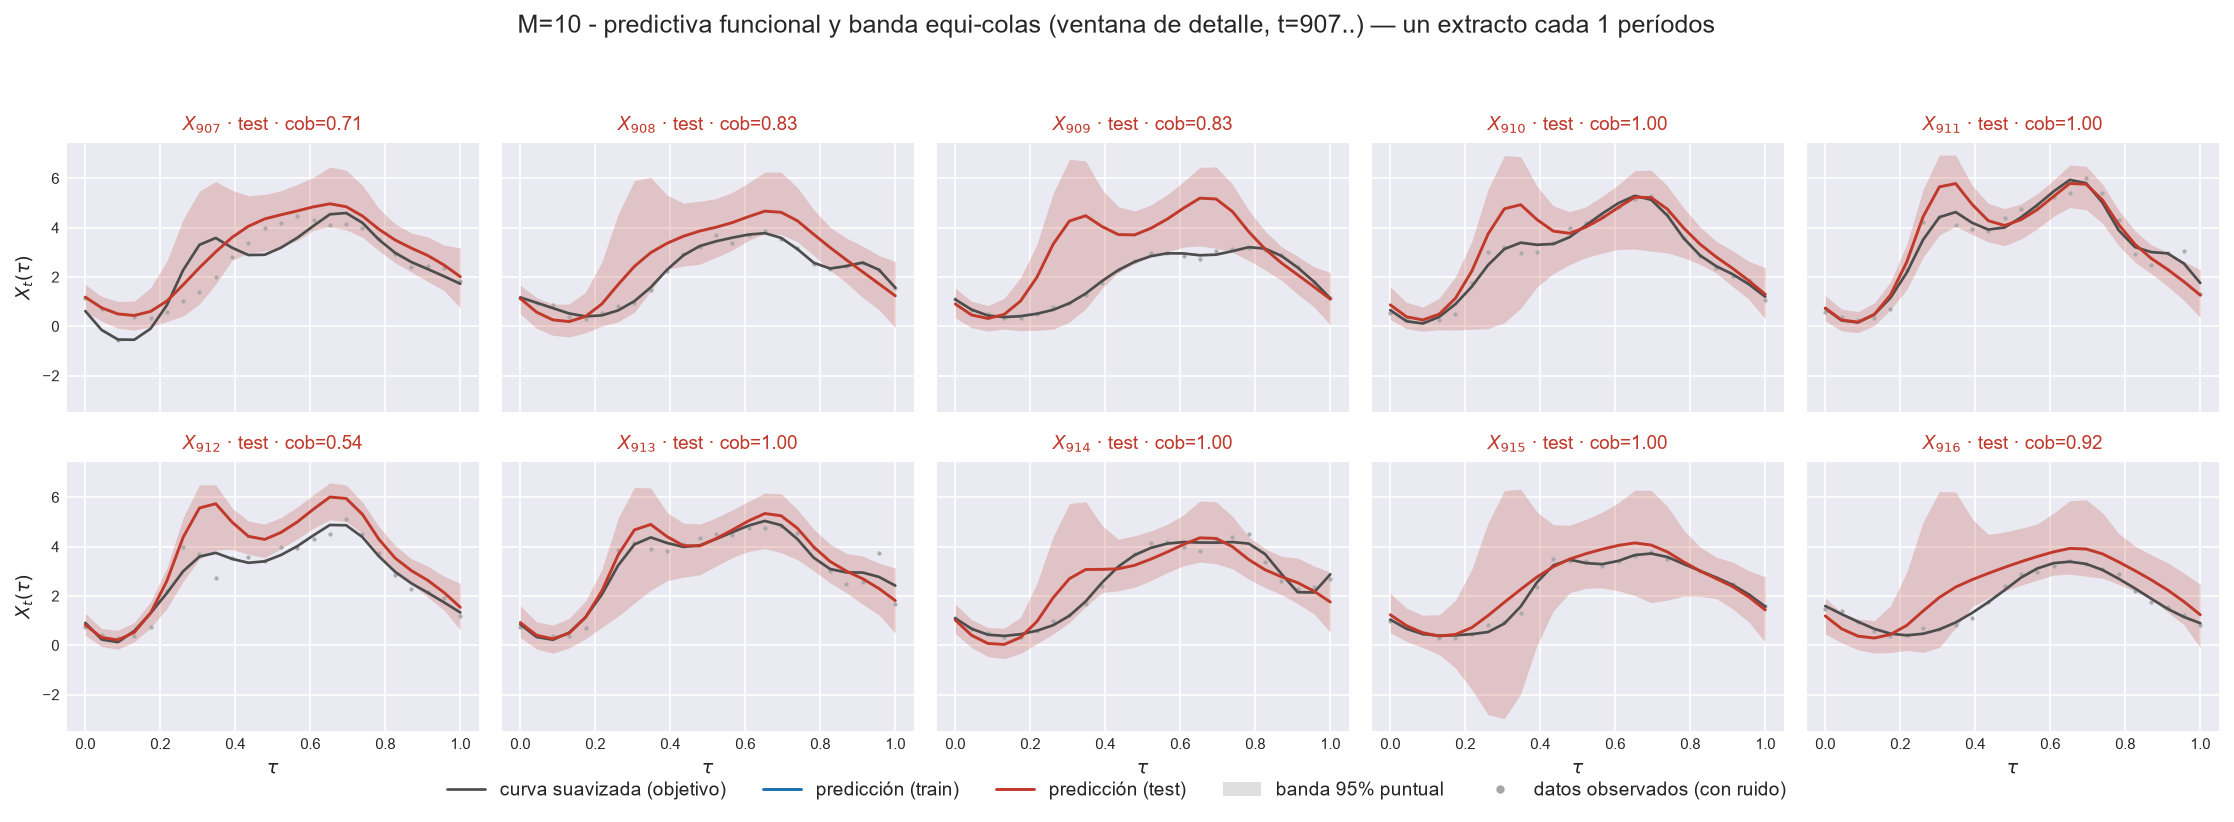
\includegraphics[width=\textwidth,height=0.8\textheight,keepaspectratio]{IMG/aneC_00/aneC_00_54_extractos_curvas_test_102.png}
\caption{Extractos de predicciones del bloque de prueba, tráfico con rezagos $\{1,7\}$ ($M = 10$).}
\label{fig:aneC_54_extractos_curvas_test_102}
\end{figure}

\begin{figure}[H]
\centering
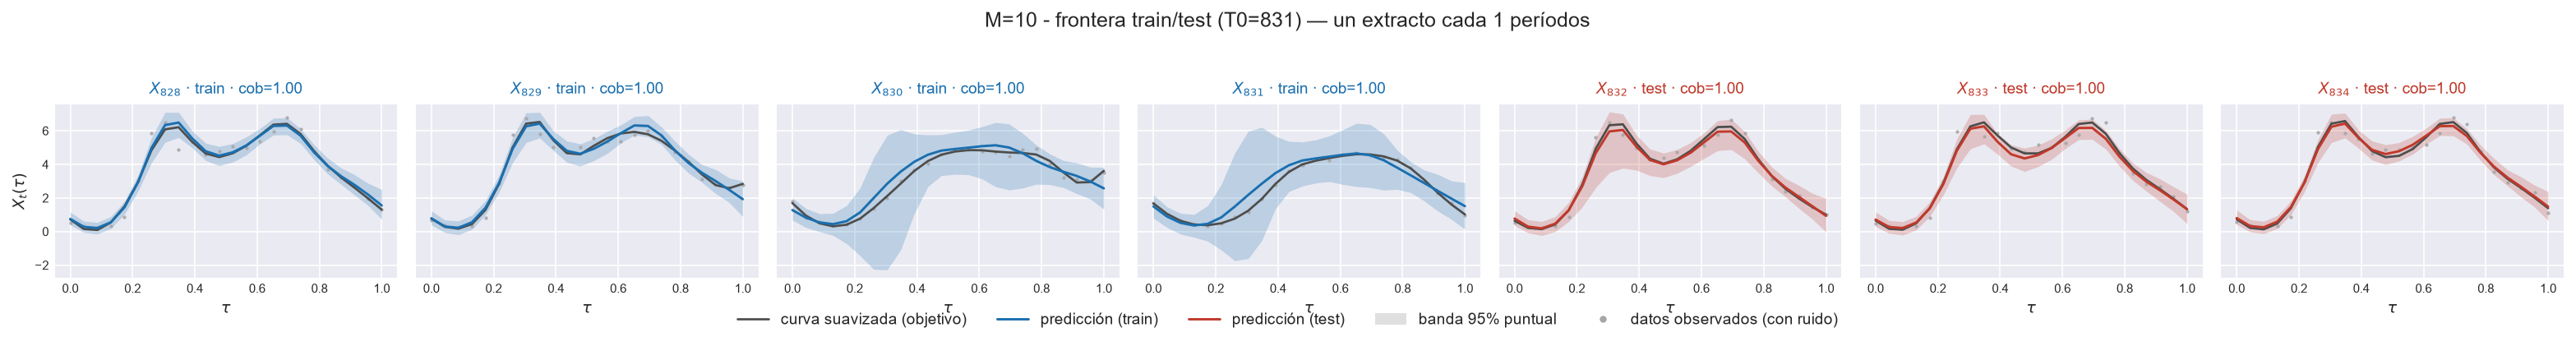
\includegraphics[width=\textwidth,height=0.8\textheight,keepaspectratio]{IMG/aneC_00/aneC_00_55_extractos_frontera_102.png}
\caption{Predicciones en la frontera entre los bloques de entrenamiento y de prueba, tráfico con rezagos $\{1,7\}$ ($M = 10$).}
\label{fig:aneC_55_extractos_frontera_102}
\end{figure}

\begin{figure}[H]
\centering
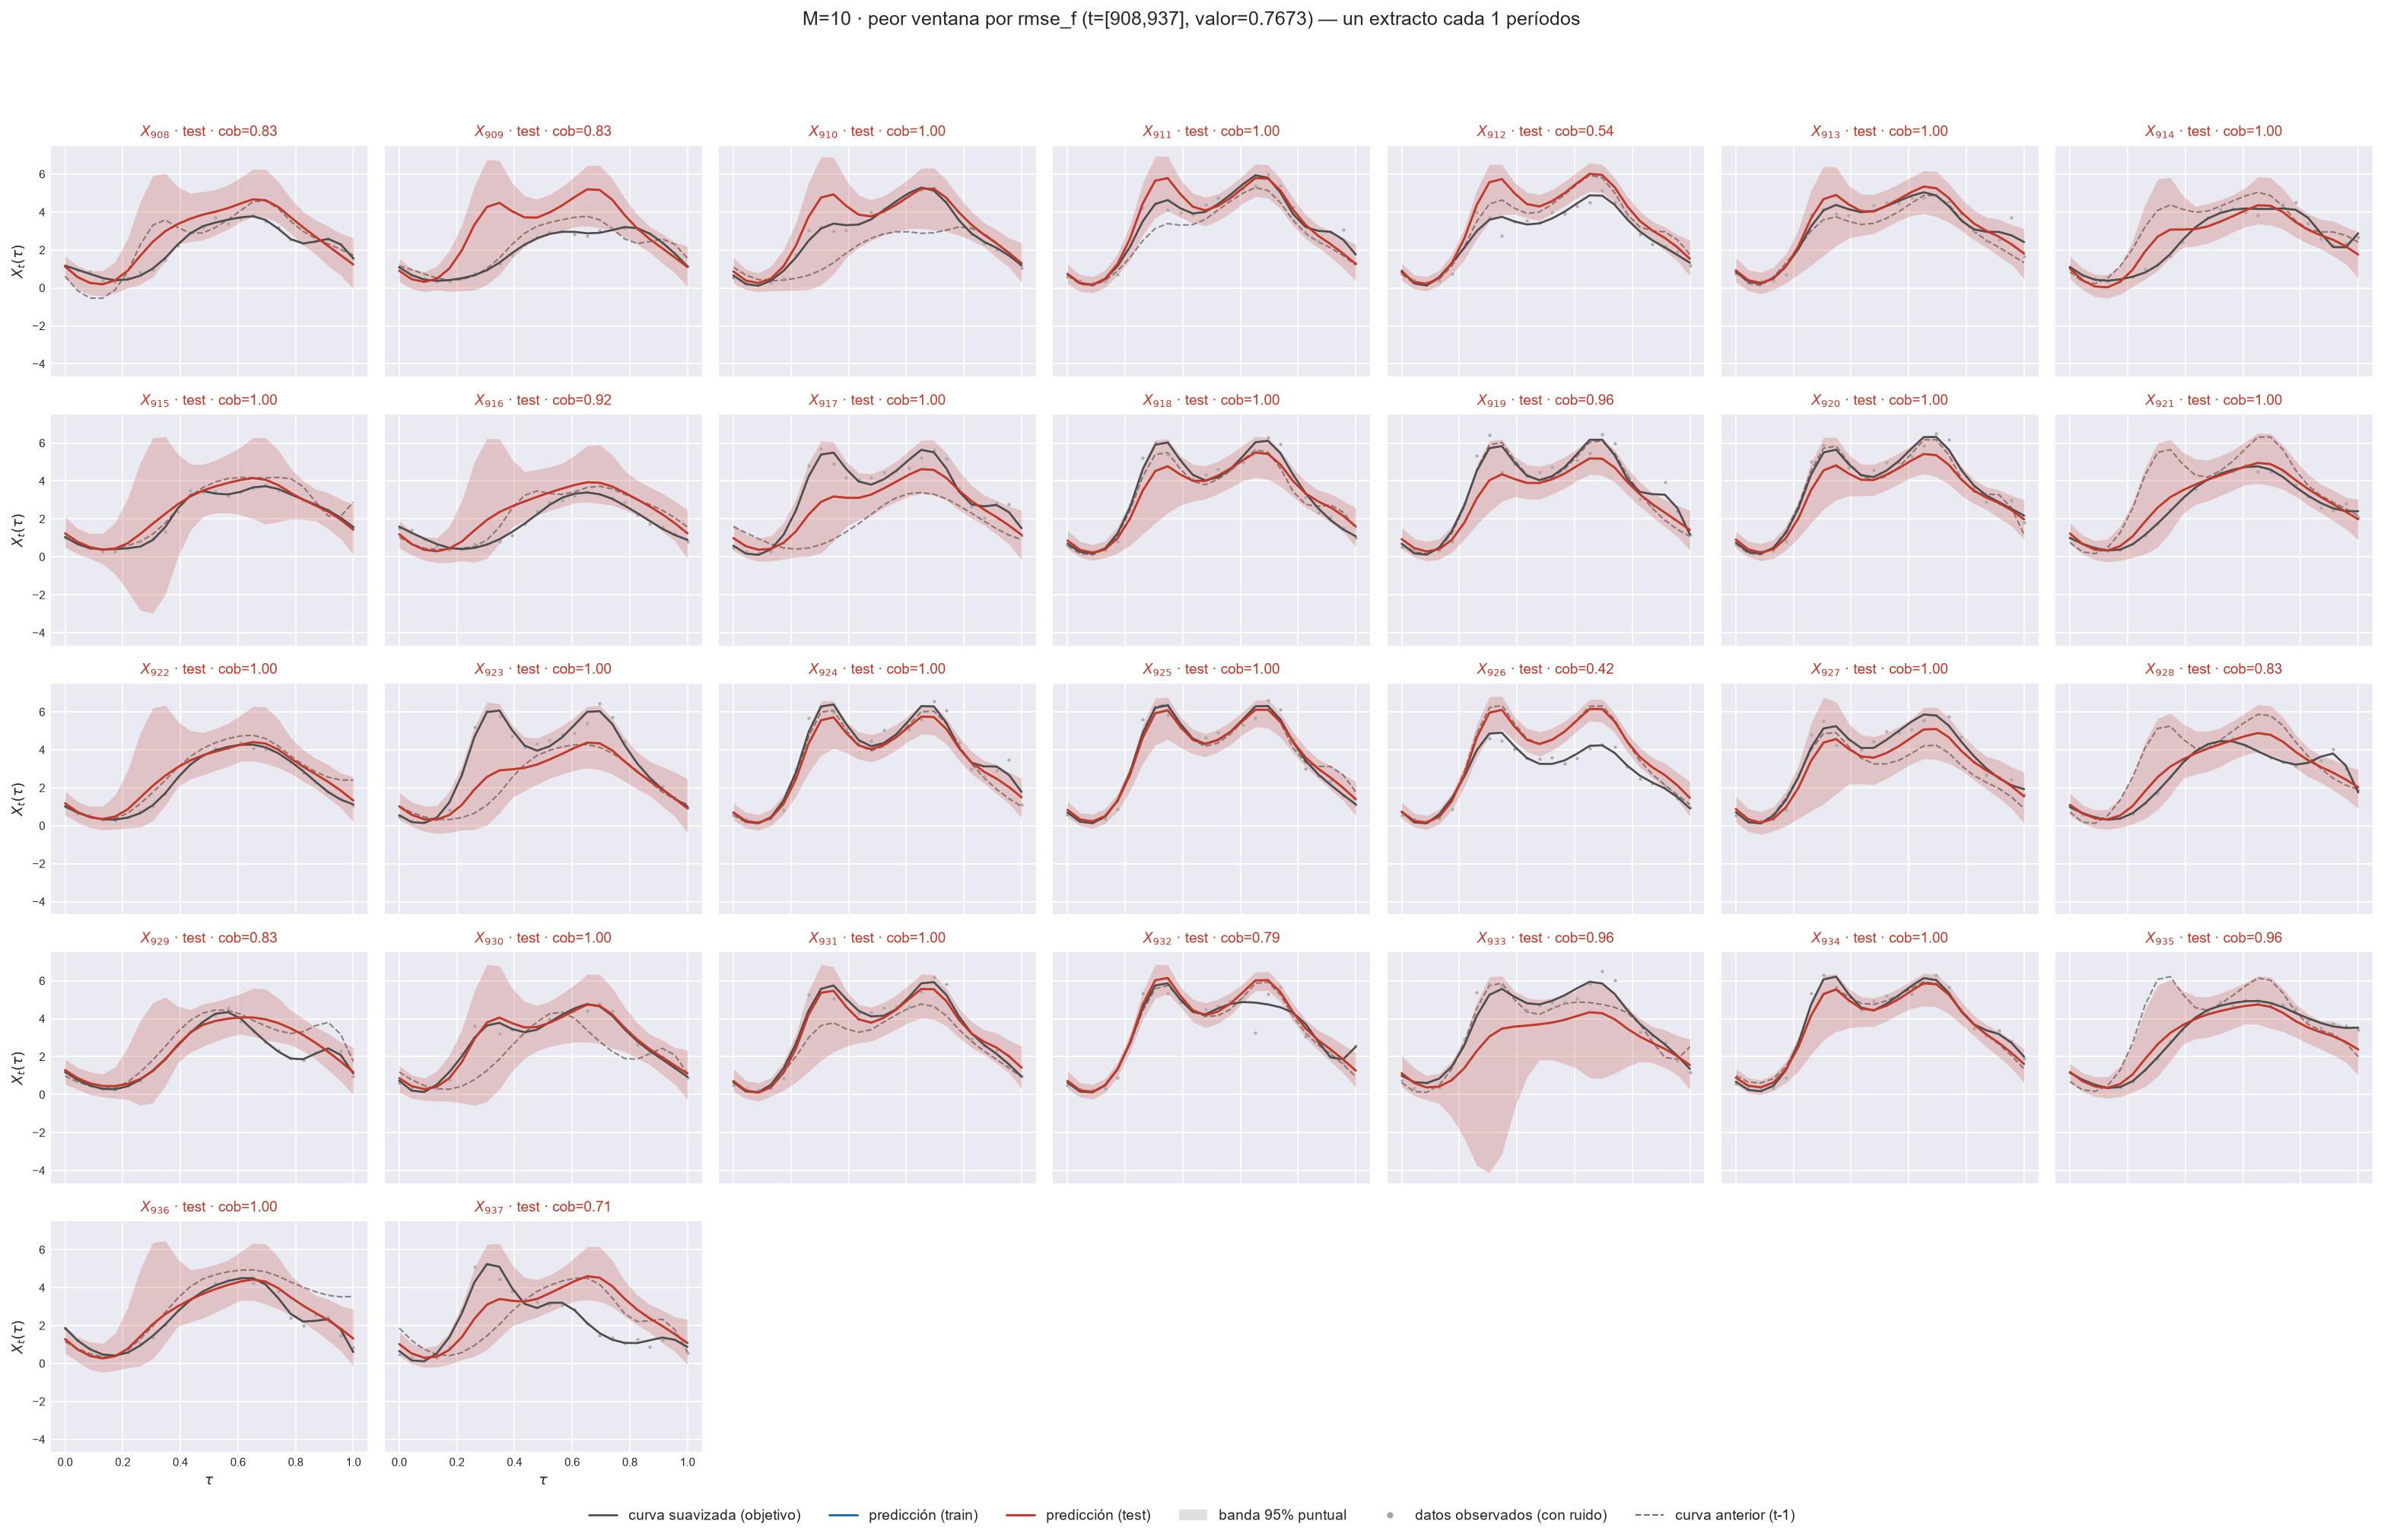
\includegraphics[width=\textwidth,height=0.8\textheight,keepaspectratio]{IMG/aneC_00/aneC_00_56b_peor_ventana_rmse_f_t908_102.png}
\caption{Ventana de peor RMSE (origen $t = 908$), tráfico con rezagos $\{1,7\}$ ($M = 10$).}
\label{fig:aneC_56b_peor_ventana_rmse_f_t908_102}
\end{figure}

\begin{figure}[H]
\centering
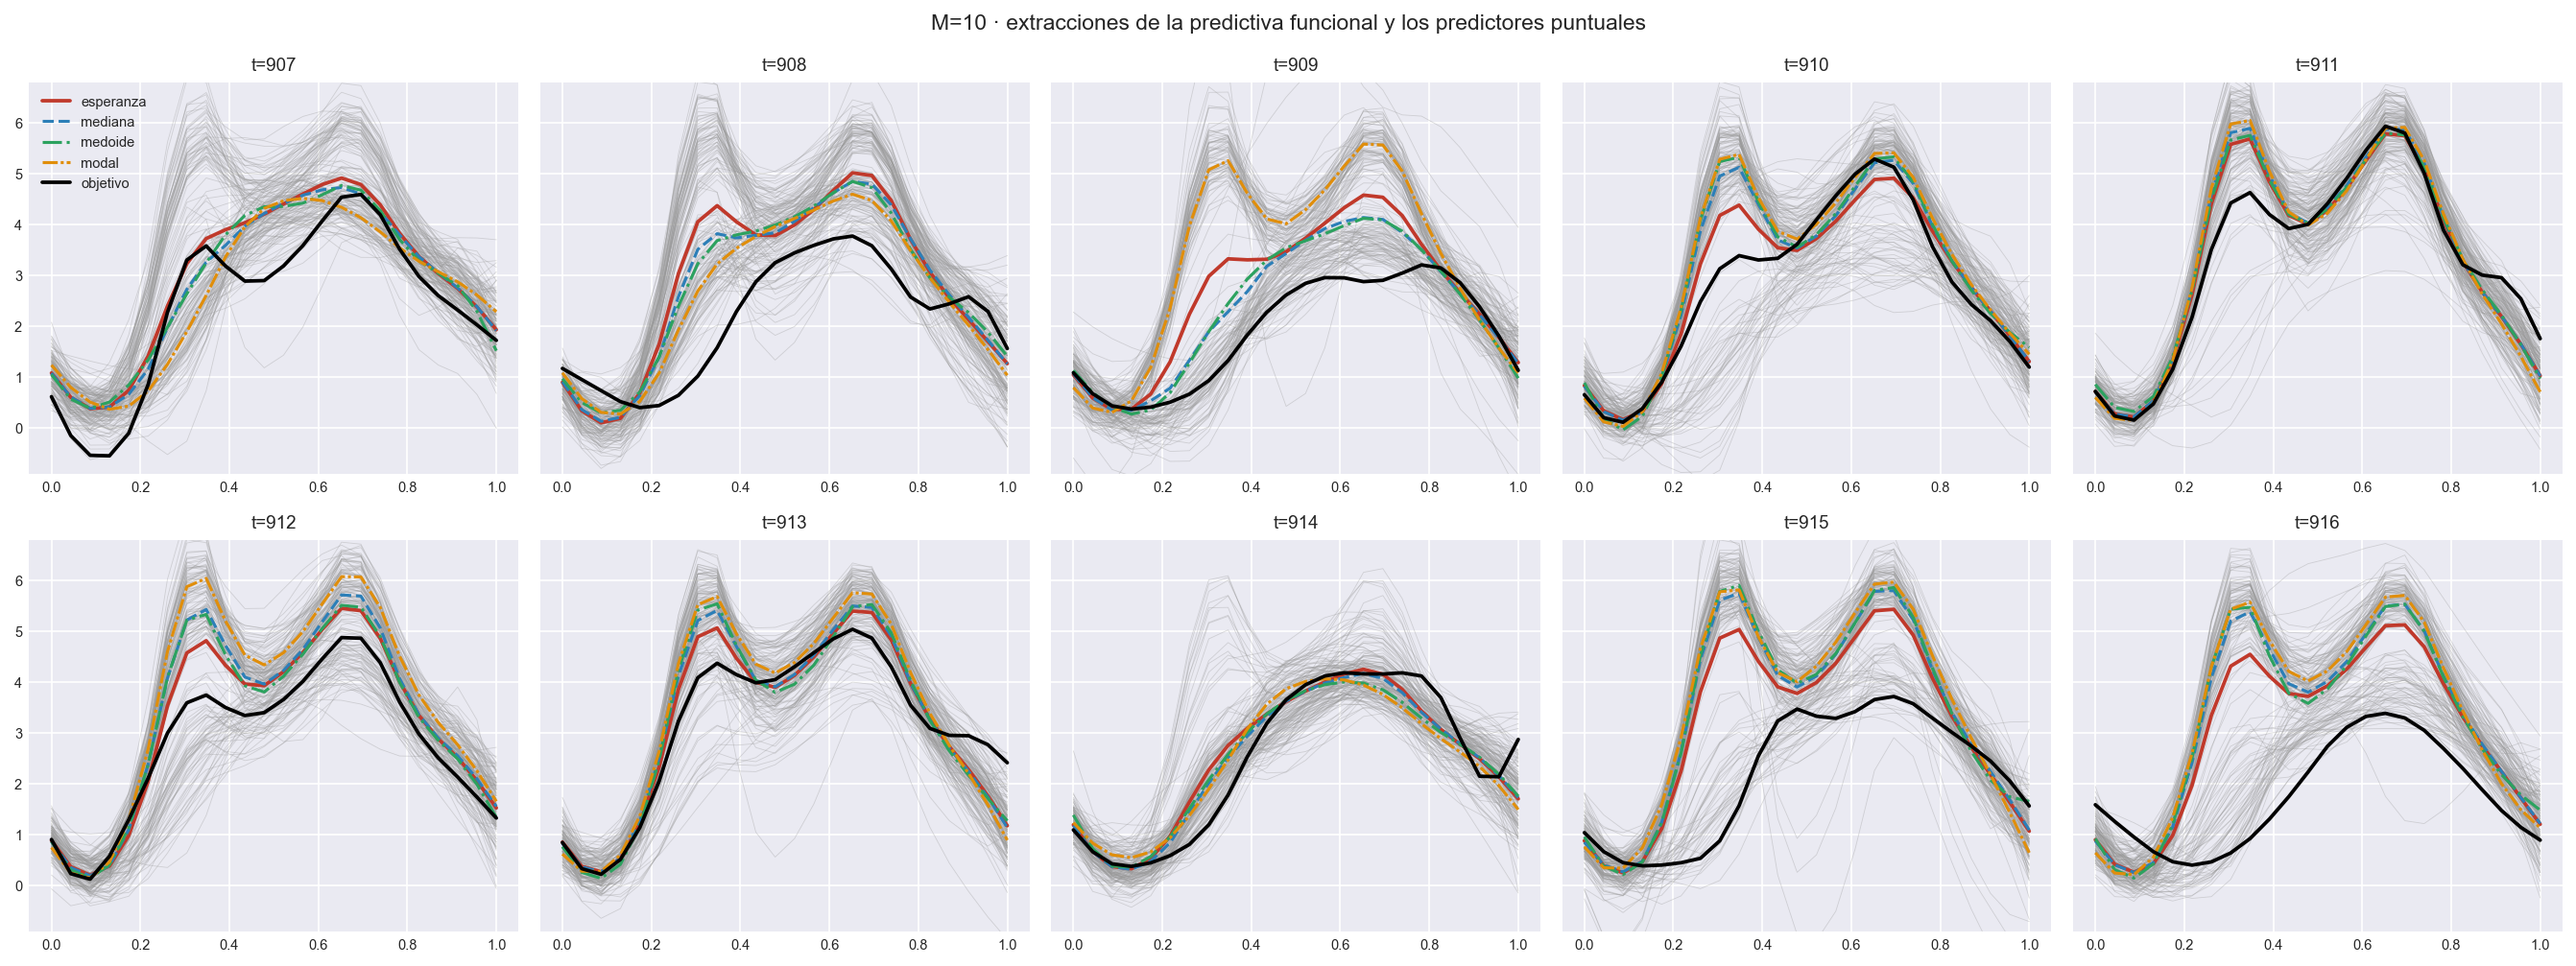
\includegraphics[width=\textwidth]{IMG/aneC_00/aneC_00_61b_curvas_predictores_101.png}
\caption{Esperanza, mediana puntual y átomo más probable en cuatro orígenes de la ventana de detalle, con la banda equi-colas y la curva observada, tráfico con rezago $\{1\}$ ($M = 10$).}
\label{fig:aneC_predictores_101}
\end{figure}

\begin{figure}[H]
\centering
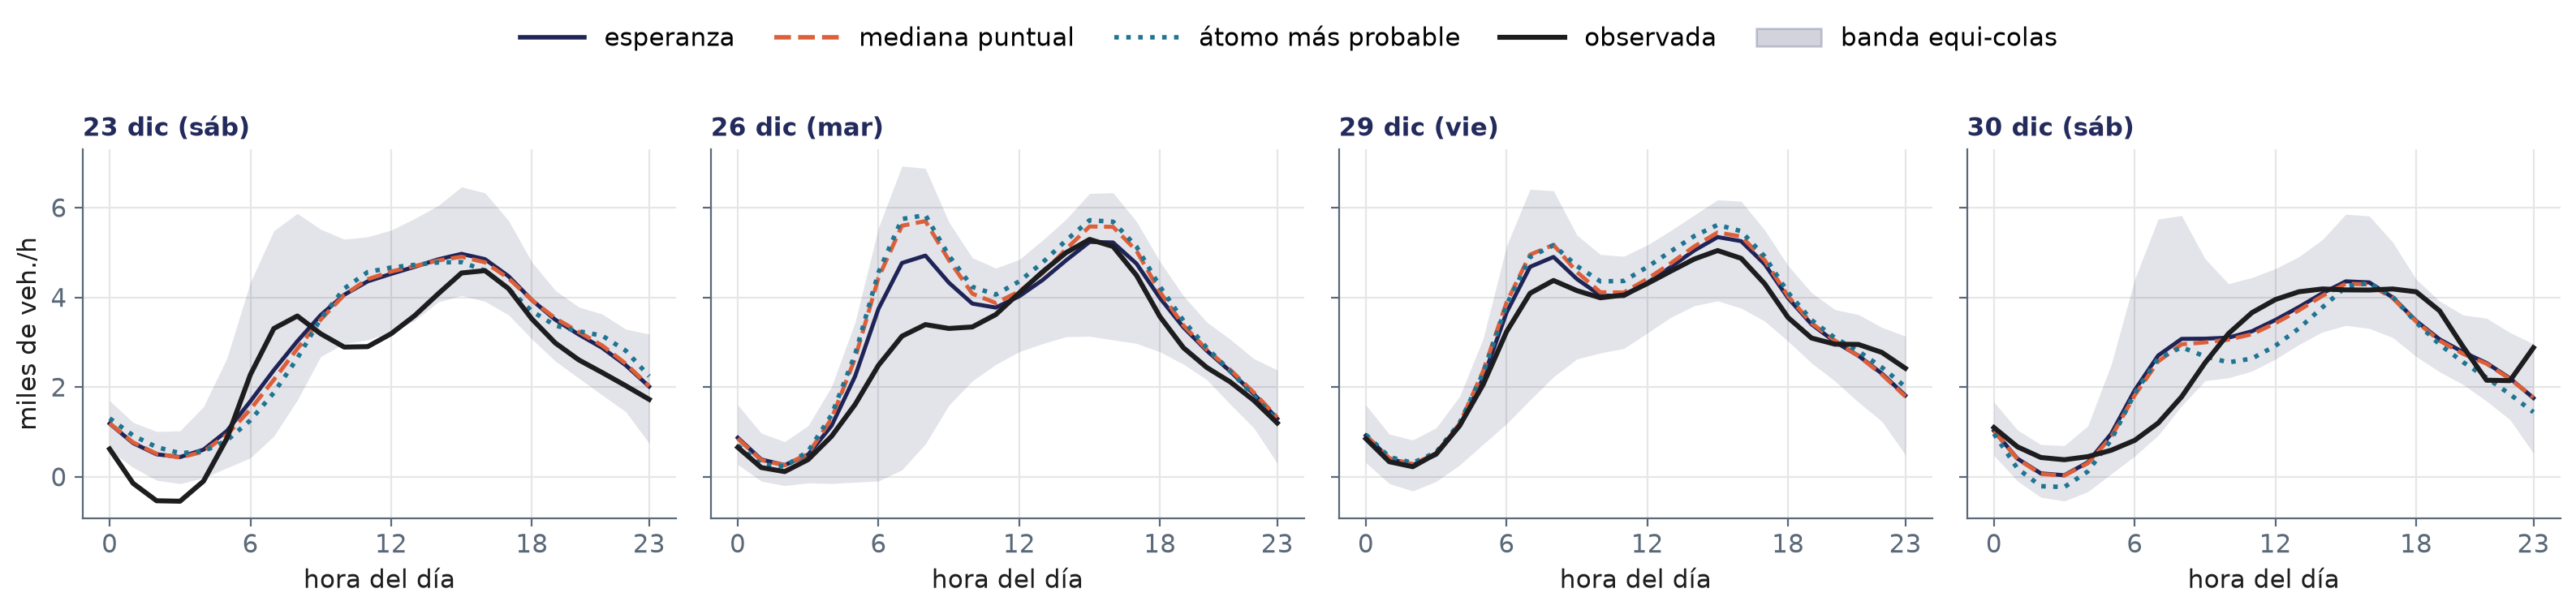
\includegraphics[width=\textwidth]{IMG/aneC_00/aneC_00_61b_curvas_predictores_102.png}
\caption{Esperanza, mediana puntual y átomo más probable en cuatro orígenes de la ventana de detalle, con la banda equi-colas y la curva observada, tráfico con rezagos $\{1,7\}$ ($M = 10$).}
\label{fig:aneC_predictores_102}
\end{figure}

\section{Comportamientos predictivos}
\label{aneC_00_06_comportamientos}

Esta sección complementa la Sección~\ref{04_03_03_comportamientos}: el número de comportamientos a lo largo del bloque de prueba, su transición entre especificaciones, los feriados, las extracciones y el catálogo de comportamientos, y los diez orígenes de la ventana de detalle.

% Fuente: K de comportamientos_psbp.npz y calendario de 65_comportamientos_calendario.csv (test).
\begin{figure}[H]
\centering
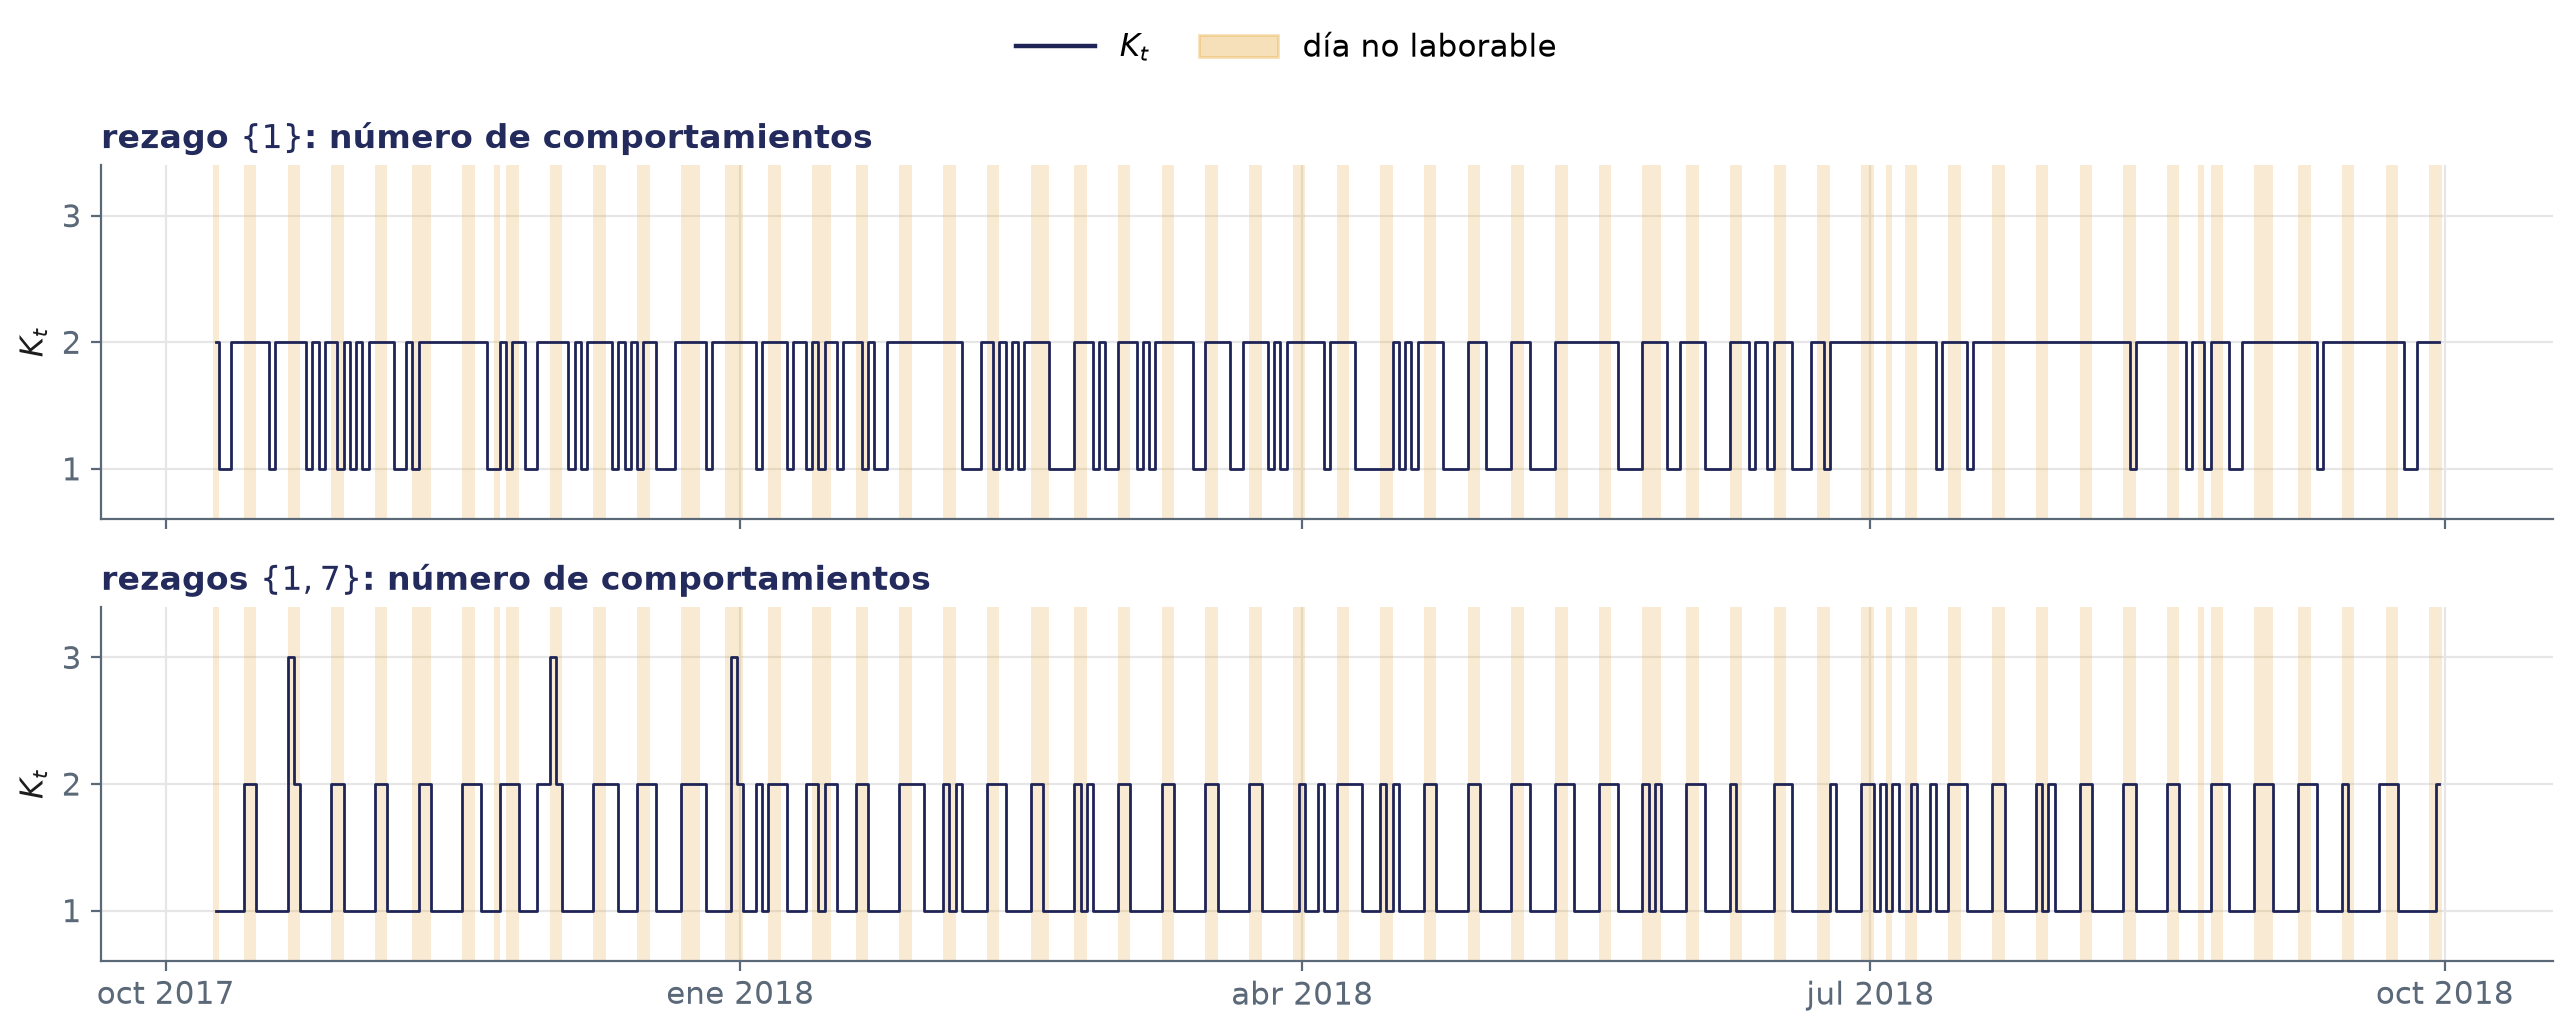
\includegraphics[width=\textwidth]{IMG/aneC_00/aneC_00_102b_K_serie.png}
\caption{Número de comportamientos $K_t$ en cada origen de prueba, con los días no laborables marcados, con rezago $\{1\}$ (arriba) y rezagos $\{1,7\}$ (abajo) ($M = 10$).}
\label{fig:aneC_Kserie}
\end{figure}

El Cuadro~\ref{tab:aneC_transicion} cruza el número de comportamientos de cada origen de prueba en las dos especificaciones. De los 256 orígenes con dos comportamientos con el rezago de un día, 139 pasan a tener uno solo al agregar el rezago semanal y 114 los conservan, mientras que solo 11 de los 101 orígenes con un comportamiento ganan un segundo.

% Fuente: K de comportamientos_psbp.npz de 101 y 102 (test, mismos 357 orígenes).
\begin{table}[H]
\centering\small
\caption{Número de comportamientos por origen de prueba con rezago $\{1\}$ (filas) y con rezagos $\{1,7\}$ (columnas) ($M = 10$).}
\label{tab:aneC_transicion}
\begin{tabular}{l ccc c}
\hline
 & $K_t = 1$ & $K_t = 2$ & $K_t = 3$ & Total \\
\hline
$K_t = 1$ & 90  & 11  & 0 & 101 \\
$K_t = 2$ & 139 & 114 & 3 & 256 \\
\hline
Total     & 229 & 125 & 3 & 357 \\
\hline
\end{tabular}
\end{table}

El Cuadro~\ref{tab:aneC_feriados} muestra el número de comportamientos en los once feriados del bloque de prueba. Con el rezago de un día nueve de ellos tienen dos comportamientos. Con el rezago semanal conservan dos comportamientos cinco feriados, todos en lunes, y pasan a uno los dos de mitad de semana y dos lunes; un solo comportamiento no implica que el perfil sea el correcto, porque en esos días la semana anterior anuncia un día laborable.

% Fuente: 65_comportamientos_calendario.csv y K de comportamientos_psbp.npz de 101 y 102.
\begin{table}[H]
\centering\small
\caption{Número de comportamientos en los feriados del bloque de prueba ($M = 10$).}
\label{tab:aneC_feriados}
\begin{tabular}{l l l cc}
\hline
Fecha & Día & Feriado & $\{1\}$ & $\{1,7\}$ \\
\hline
9 oct 2017  & lunes     & Columbus Day              & 2 & 1 \\
10 nov 2017 & viernes   & Veterans Day              & 1 & 1 \\
23 nov 2017 & jueves    & Thanksgiving Day          & 1 & 1 \\
25 dic 2017 & lunes     & Christmas Day             & 2 & 2 \\
1 ene 2018  & lunes     & New Year's Day            & 2 & 2 \\
15 ene 2018 & lunes     & Martin Luther King Jr Day & 2 & 2 \\
19 feb 2018 & lunes     & Washington's Birthday     & 2 & 1 \\
28 may 2018 & lunes     & Memorial Day              & 2 & 2 \\
4 jul 2018  & miércoles & Independence Day          & 2 & 1 \\
23 ago 2018 & jueves    & State Fair                & 2 & 1 \\
3 sep 2018  & lunes     & Labor Day                 & 2 & 2 \\
\hline
\end{tabular}
\end{table}

\begin{figure}[H]
\centering
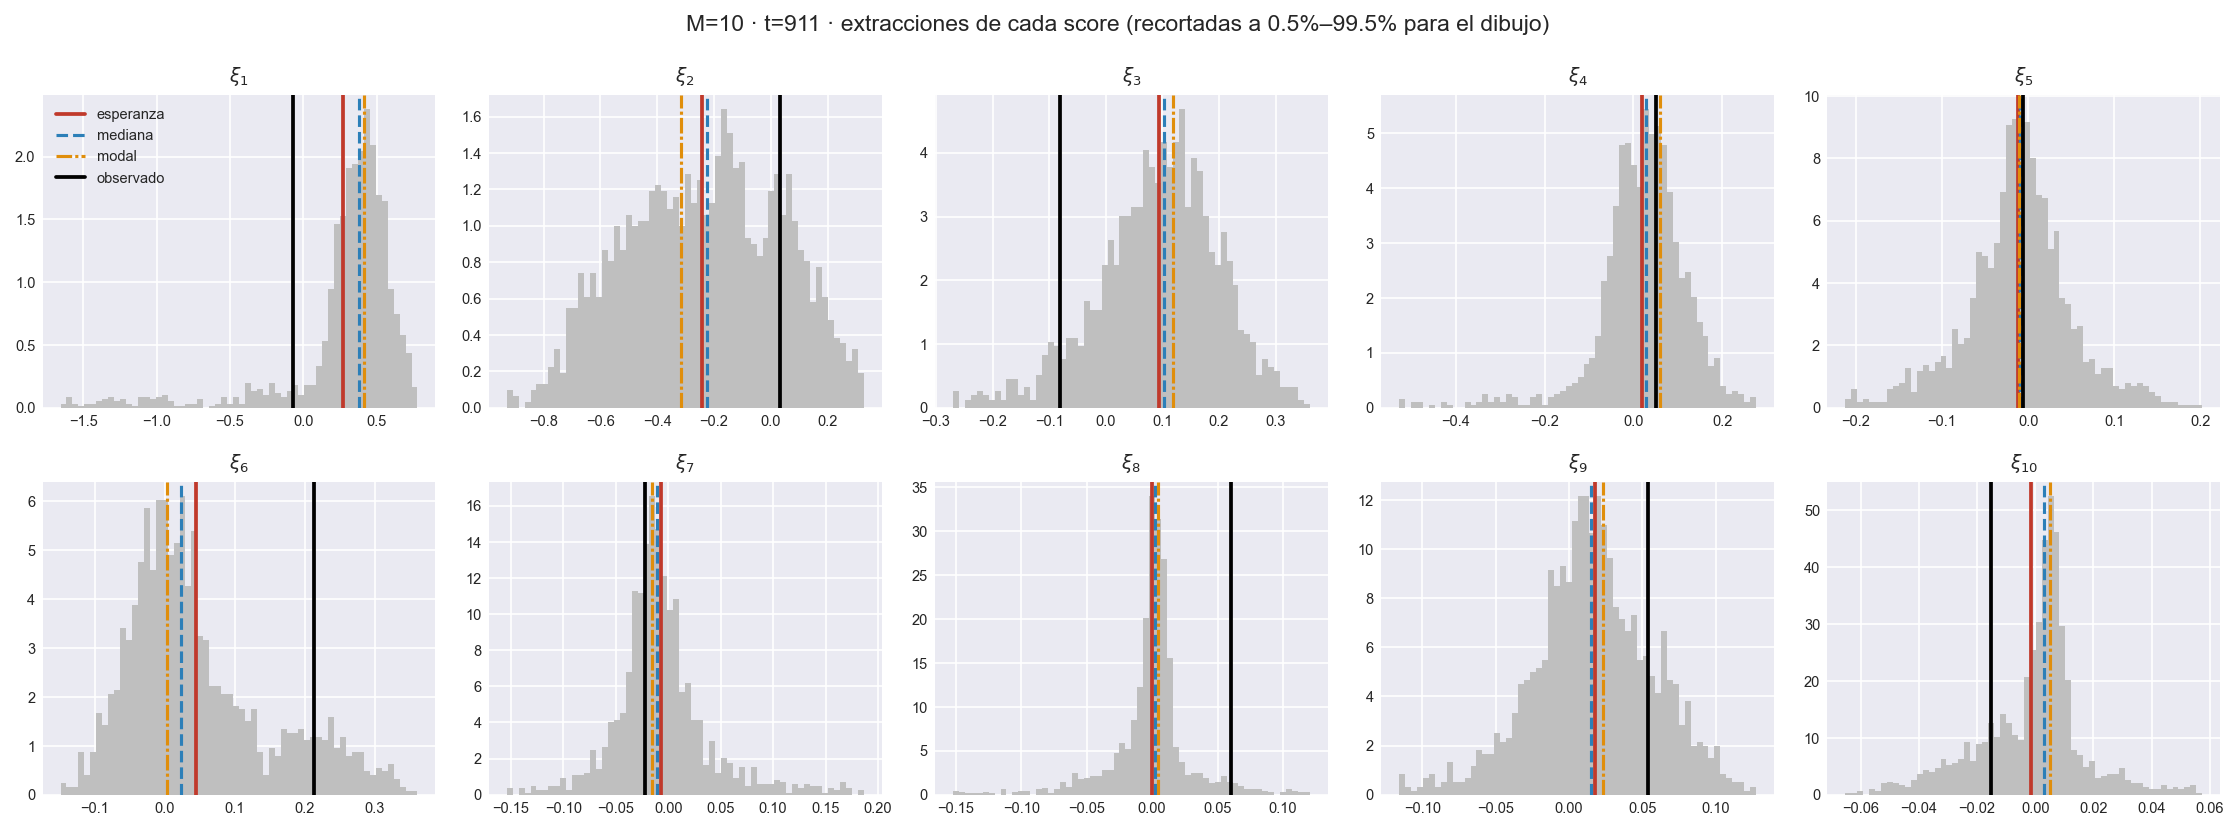
\includegraphics[width=\textwidth,height=0.6\textheight,keepaspectratio]{IMG/aneC_00/aneC_00_61_histogramas_draws_101.png}
\caption{Histograma de las extracciones del score en un origen con más de un comportamiento, tráfico con rezago $\{1\}$ ($M = 10$).}
\label{fig:aneC_hist_101}
\end{figure}

\begin{figure}[H]
\centering
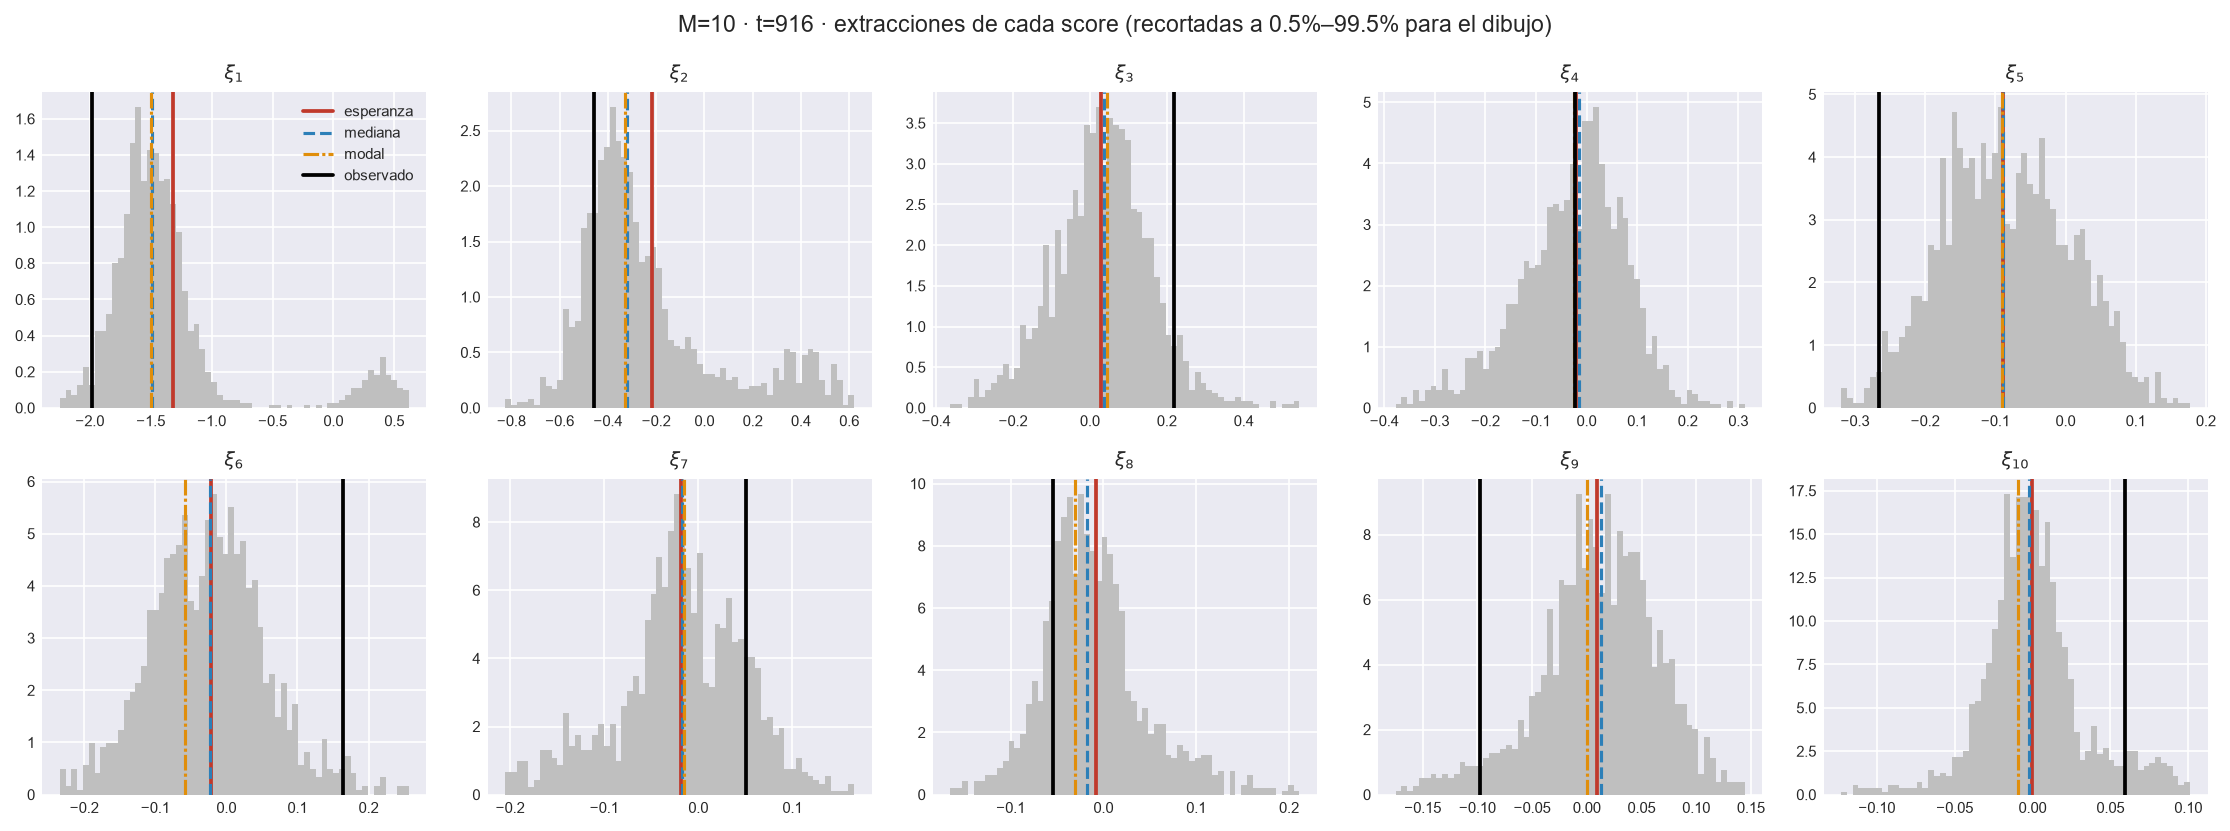
\includegraphics[width=\textwidth,height=0.6\textheight,keepaspectratio]{IMG/aneC_00/aneC_00_61_histogramas_draws_102.png}
\caption{Histograma de las extracciones del score en un origen con más de un comportamiento, tráfico con rezagos $\{1,7\}$ ($M = 10$).}
\label{fig:aneC_hist_102}
\end{figure}

\begin{figure}[H]
\centering
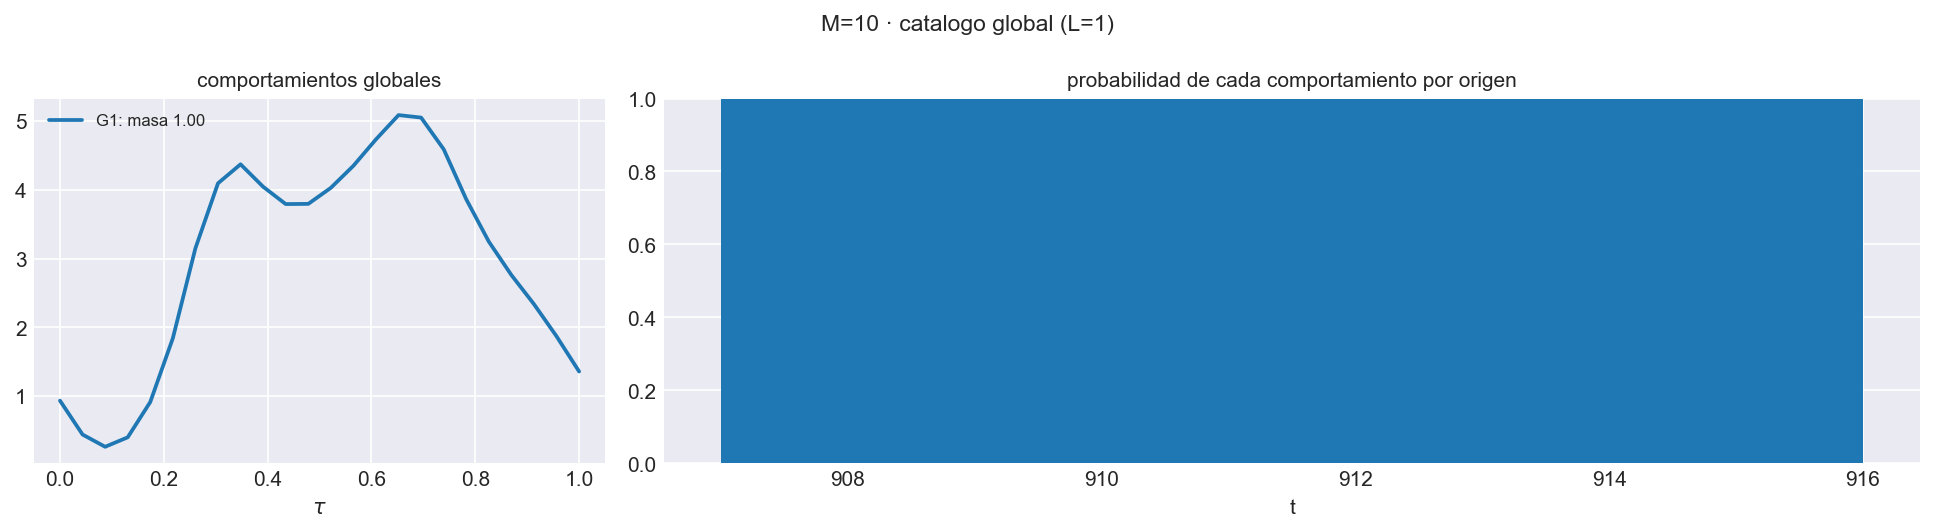
\includegraphics[width=\textwidth,height=0.6\textheight,keepaspectratio]{IMG/aneC_00/aneC_00_64_catalogo_global_101.png}
\caption{Catálogo global de comportamientos, tráfico con rezago $\{1\}$ ($M = 10$).}
\label{fig:aneC_catalogo_101}
\end{figure}

\begin{figure}[H]
\centering
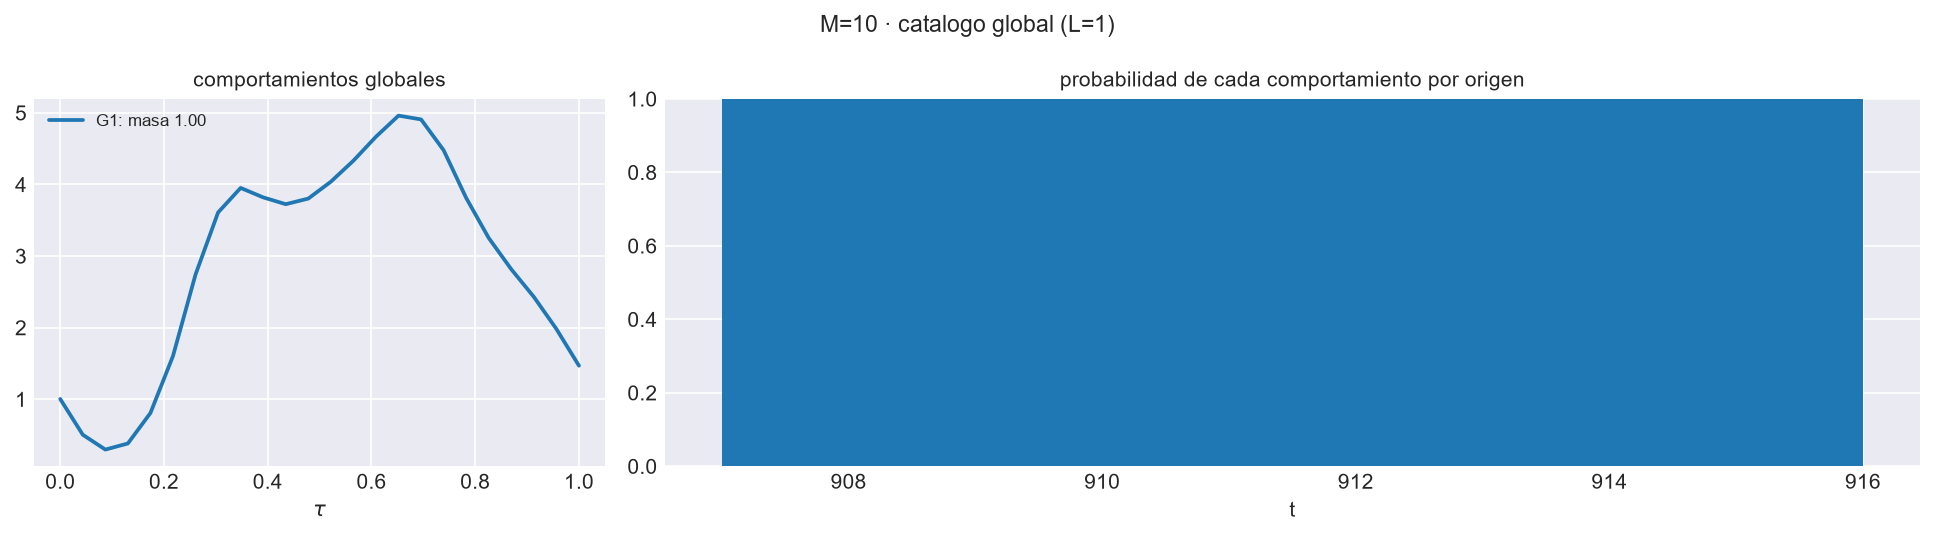
\includegraphics[width=\textwidth,height=0.6\textheight,keepaspectratio]{IMG/aneC_00/aneC_00_64_catalogo_global_102.png}
\caption{Catálogo global de comportamientos, tráfico con rezagos $\{1,7\}$ ($M = 10$).}
\label{fig:aneC_catalogo_102}
\end{figure}

% Fuente: comportamientos_psbp.npz y banda_funcional_psbp.npz del _04 de 101 y 102, curva suavizada (theta @ phi^T).
\begin{figure}[H]
\centering
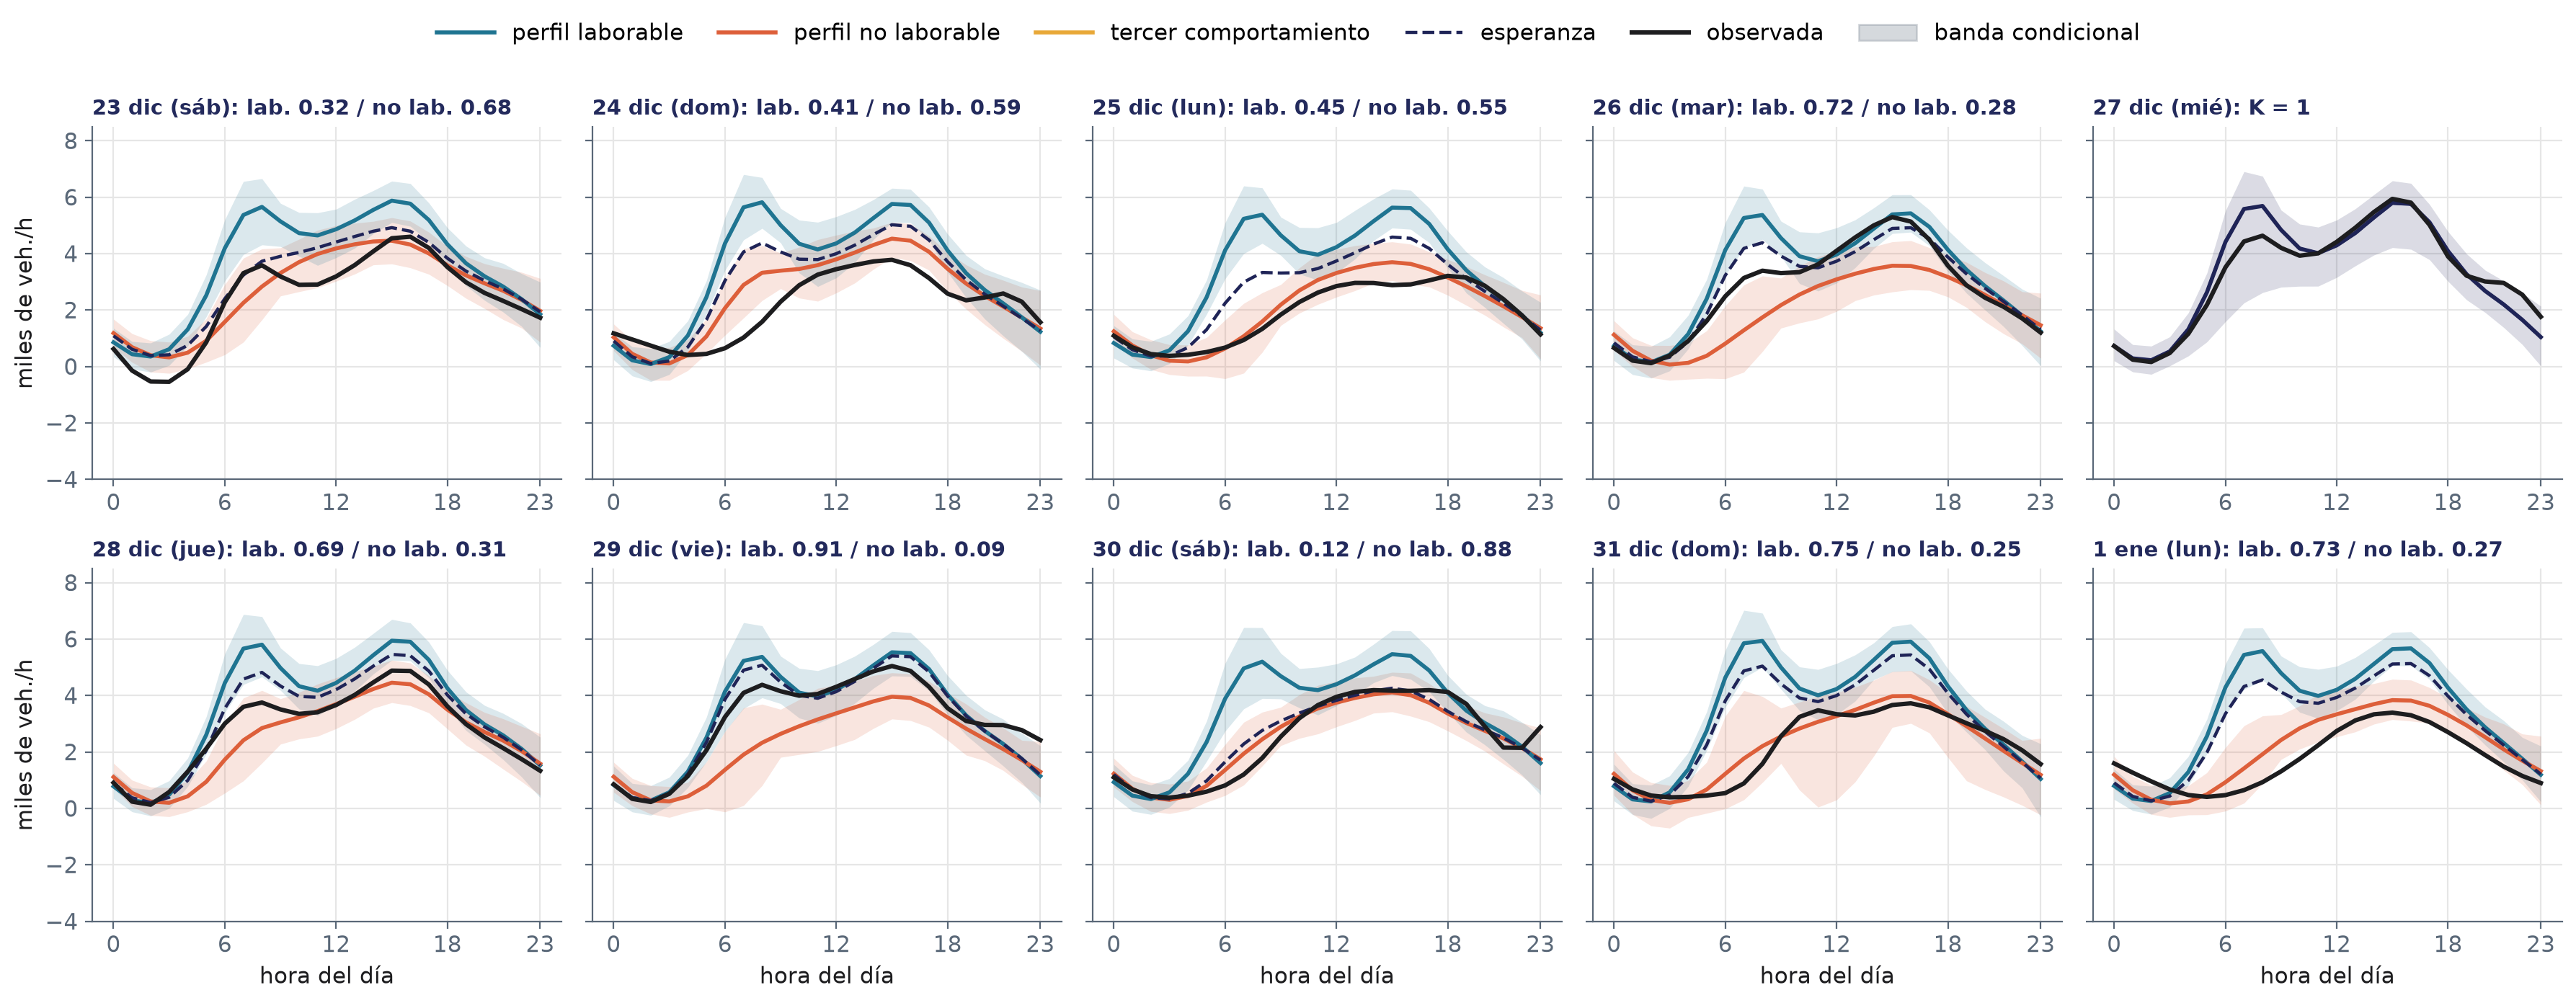
\includegraphics[width=\textwidth]{IMG/aneC_00/aneC_00_63_detalle_101.png}
\caption{Ventana de detalle completa, del 23 de diciembre de 2017 al 1 de enero de 2018, tráfico con rezago $\{1\}$ ($M = 10$): curva observada, esperanza y, por comportamiento, curva típica, banda condicional y probabilidad.}
\label{fig:aneC_detalle_101}
\end{figure}

\begin{figure}[H]
\centering
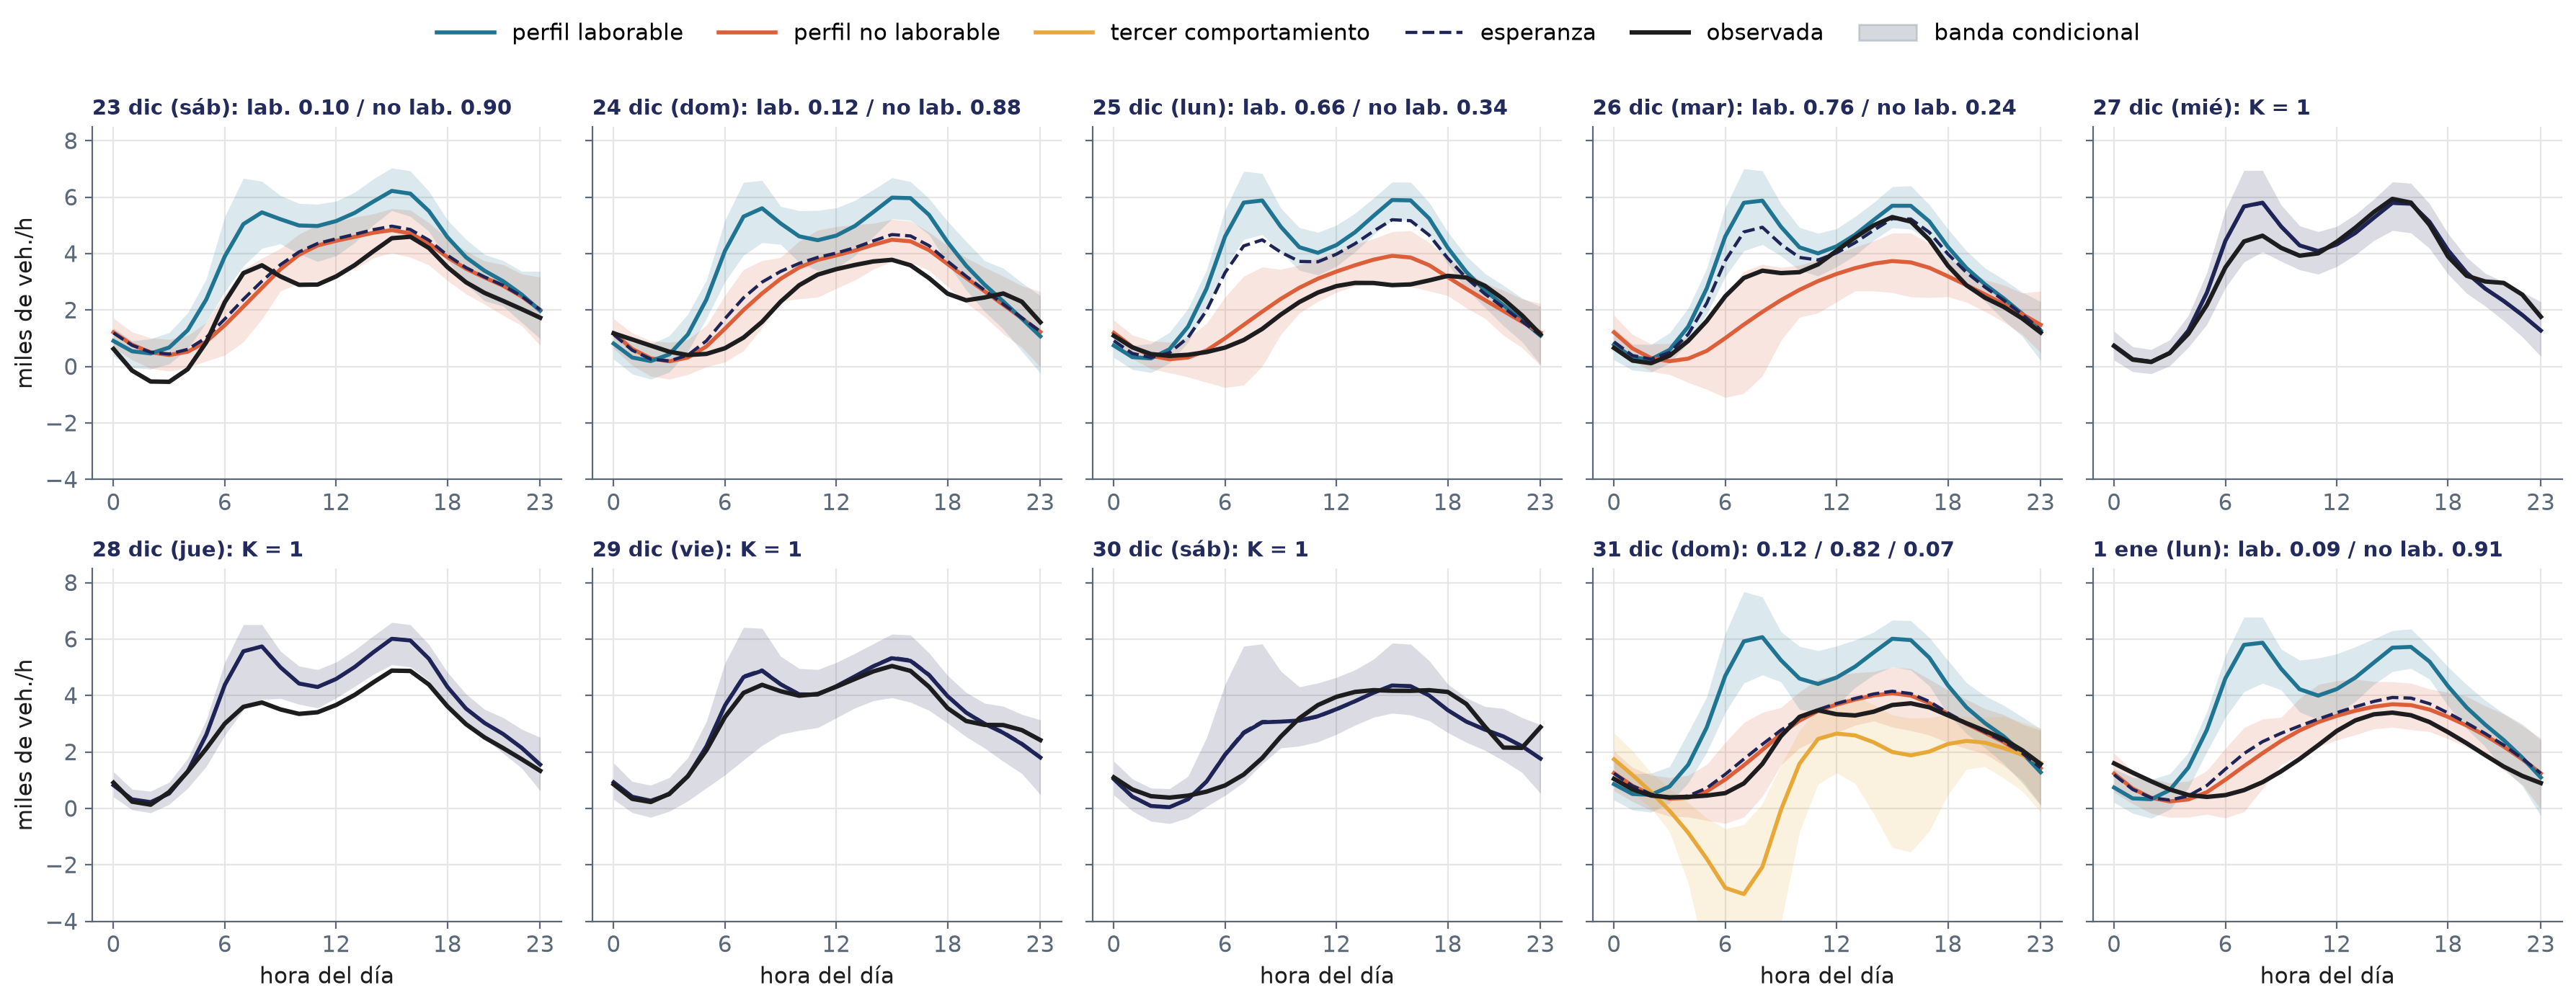
\includegraphics[width=\textwidth]{IMG/aneC_00/aneC_00_63_detalle_102.png}
\caption{Ventana de detalle completa, del 23 de diciembre de 2017 al 1 de enero de 2018, tráfico con rezagos $\{1,7\}$ ($M = 10$). Con tres comportamientos, las probabilidades van en orden de nivel.}
\label{fig:aneC_detalle_102}
\end{figure}

\section{Intervalos en la ventana de detalle}
\label{aneC_00_07_intervalos_detalle}
% 79: contraste de las bandas en la ventana de detalle.

Las tres construcciones de intervalo del PSBPM-FD y la banda del FAR en los diez orígenes de la ventana de detalle.

\begin{figure}[H]
\centering
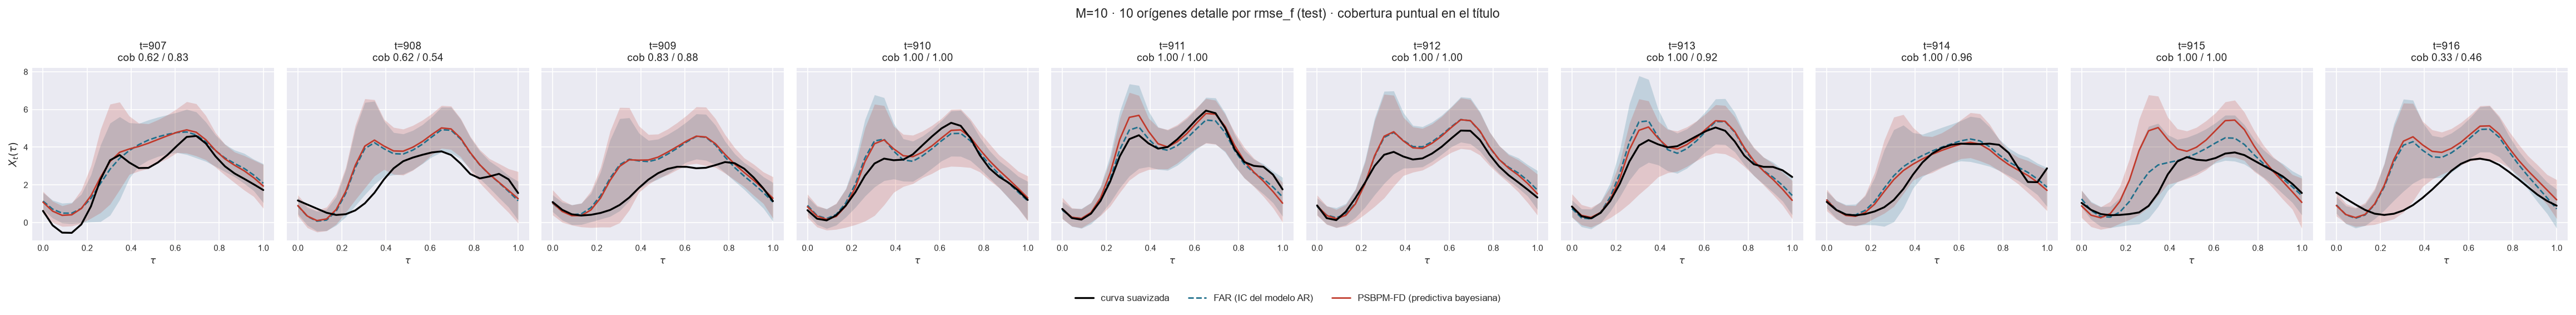
\includegraphics[width=\textwidth,height=0.75\textheight,keepaspectratio]{IMG/aneC_00/aneC_00_79_ic_contraste_detalle_101.png}
\caption{Bandas equi-colas y del FAR en la ventana de detalle, tráfico con rezago $\{1\}$ ($M = 10$).}
\label{fig:aneC_79_ic_contraste_detalle_101}
\end{figure}

\begin{figure}[H]
\centering
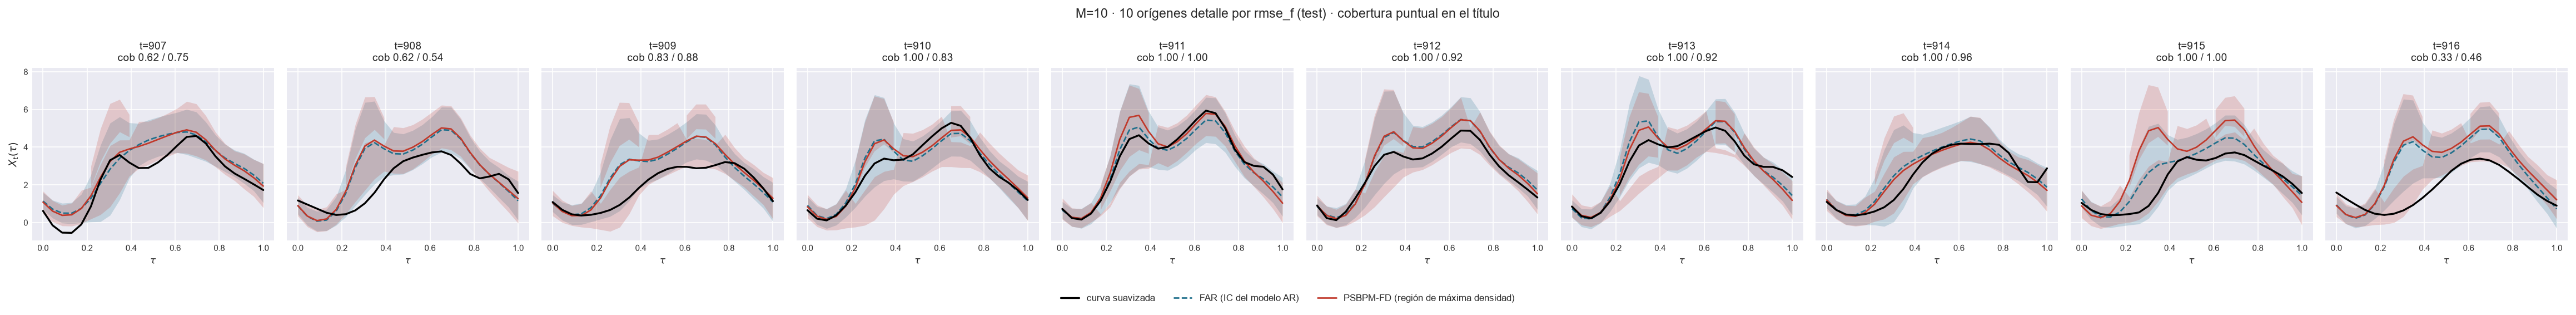
\includegraphics[width=\textwidth,height=0.75\textheight,keepaspectratio]{IMG/aneC_00/aneC_00_79_ic_contraste_detalle_hdr_101.png}
\caption{Región de máxima densidad en la ventana de detalle, tráfico con rezago $\{1\}$ ($M = 10$).}
\label{fig:aneC_79_ic_contraste_detalle_hdr_101}
\end{figure}

\begin{figure}[H]
\centering
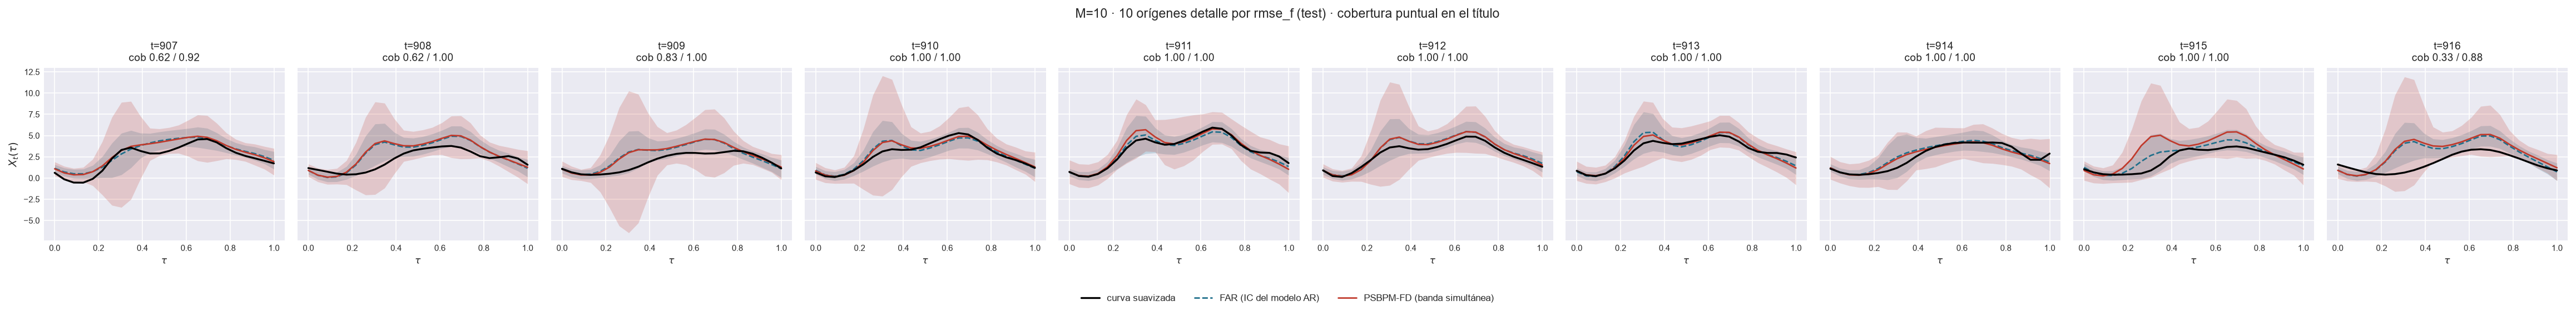
\includegraphics[width=\textwidth,height=0.75\textheight,keepaspectratio]{IMG/aneC_00/aneC_00_79_ic_contraste_detalle_simultanea_101.png}
\caption{Banda simultánea en la ventana de detalle, tráfico con rezago $\{1\}$ ($M = 10$).}
\label{fig:aneC_79_ic_contraste_detalle_simultanea_101}
\end{figure}

\begin{figure}[H]
\centering
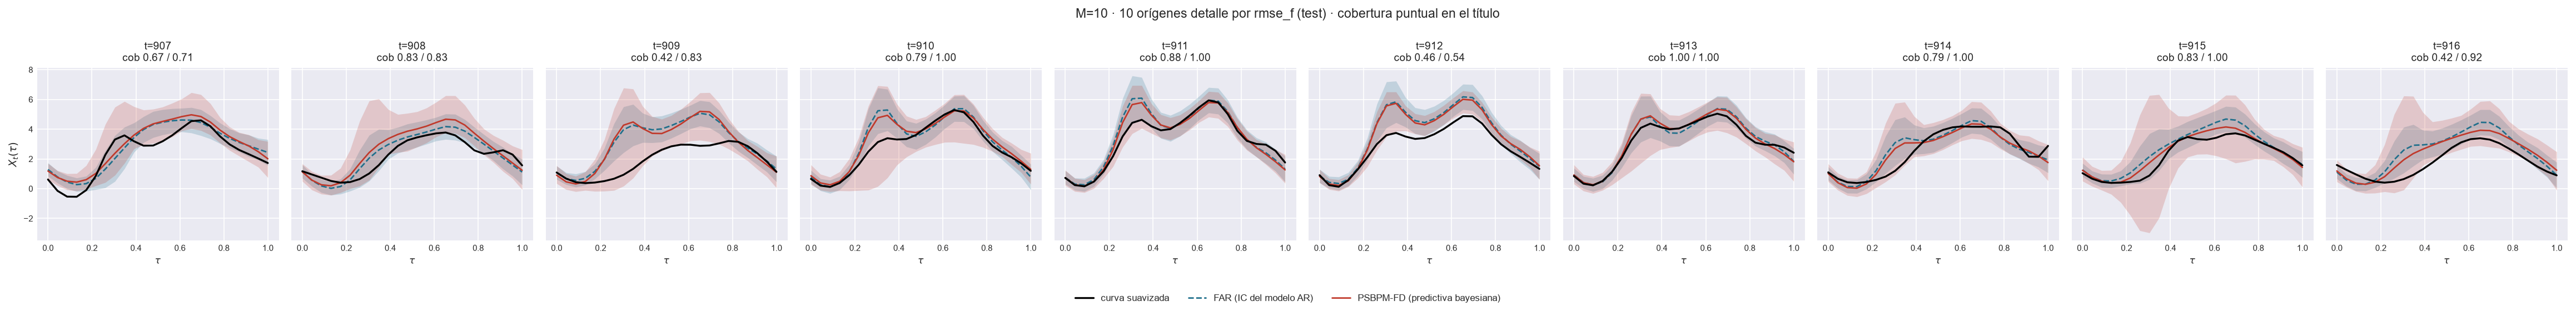
\includegraphics[width=\textwidth,height=0.75\textheight,keepaspectratio]{IMG/aneC_00/aneC_00_79_ic_contraste_detalle_102.png}
\caption{Bandas equi-colas y del FAR en la ventana de detalle, tráfico con rezagos $\{1,7\}$ ($M = 10$).}
\label{fig:aneC_79_ic_contraste_detalle_102}
\end{figure}

\begin{figure}[H]
\centering
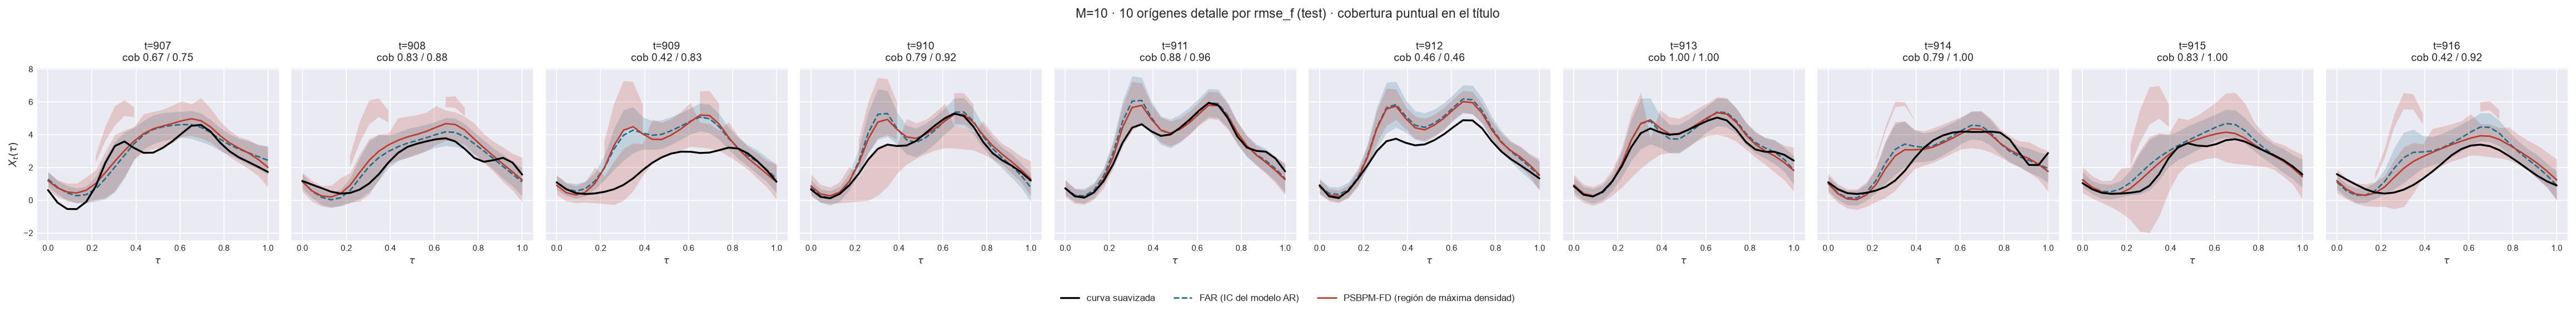
\includegraphics[width=\textwidth,height=0.75\textheight,keepaspectratio]{IMG/aneC_00/aneC_00_79_ic_contraste_detalle_hdr_102.png}
\caption{Región de máxima densidad en la ventana de detalle, tráfico con rezagos $\{1,7\}$ ($M = 10$).}
\label{fig:aneC_79_ic_contraste_detalle_hdr_102}
\end{figure}

\begin{figure}[H]
\centering
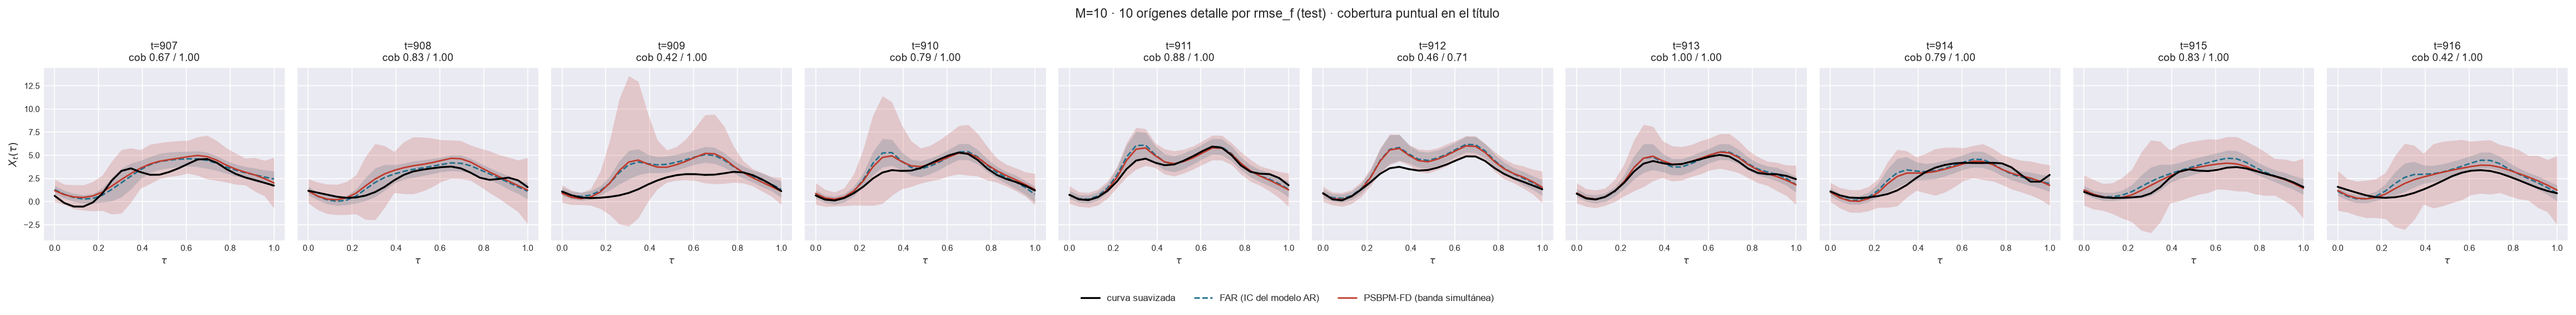
\includegraphics[width=\textwidth,height=0.75\textheight,keepaspectratio]{IMG/aneC_00/aneC_00_79_ic_contraste_detalle_simultanea_102.png}
\caption{Banda simultánea en la ventana de detalle, tráfico con rezagos $\{1,7\}$ ($M = 10$).}
\label{fig:aneC_79_ic_contraste_detalle_simultanea_102}
\end{figure}

\section{Monitoreo por componente}
\label{aneC_00_08_componentes}
% 91-94: error y banda de credibilidad de cada score, como en el Anexo B para simulación.

El error y la banda de credibilidad de cada score, como en la Sección~\ref{aneB_00_05_intervalos_componente} para la simulación.

\begin{figure}[H]
\centering
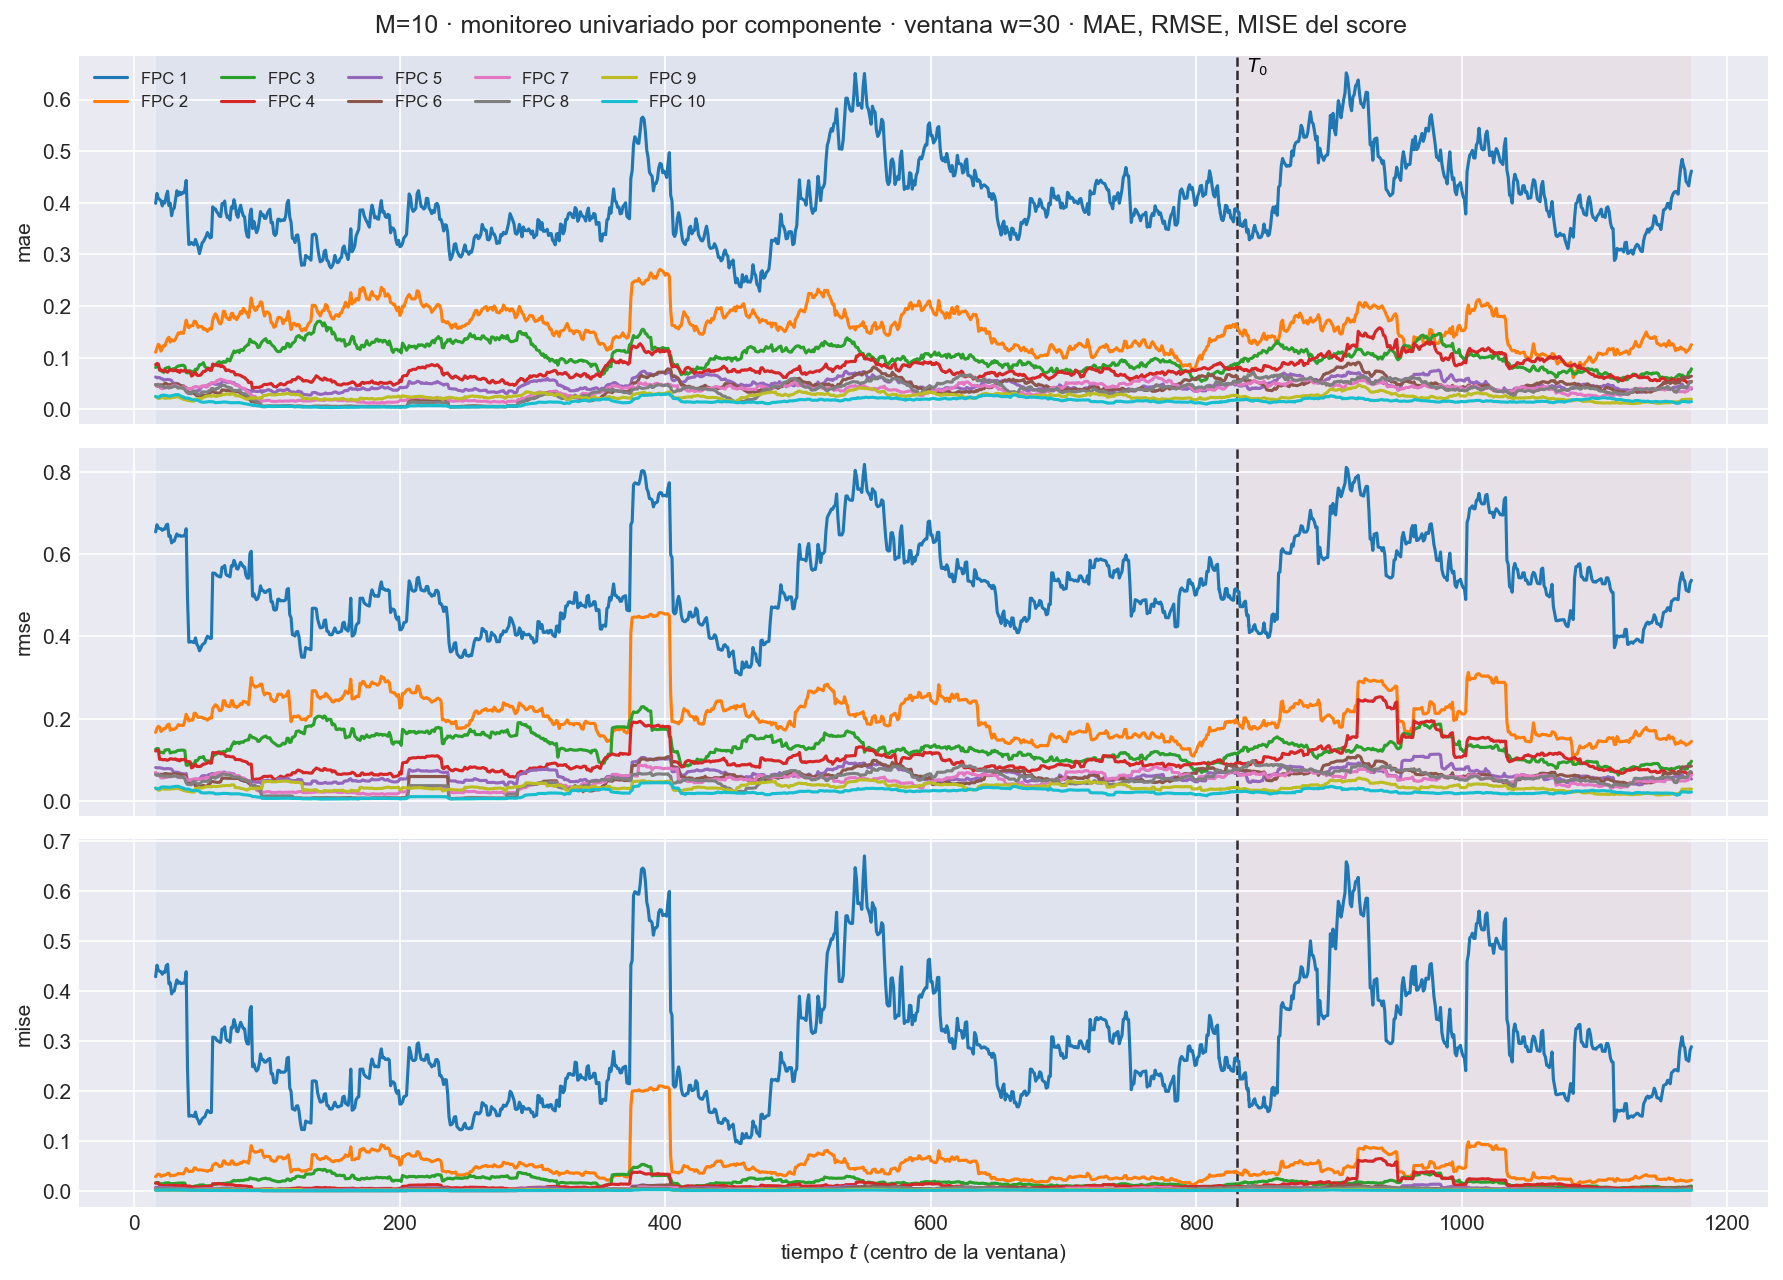
\includegraphics[width=\textwidth,height=0.75\textheight,keepaspectratio]{IMG/aneC_00/aneC_00_91_ventana_univariado_w30_101.png}
\caption{Error de cada score sobre la ventana móvil, tráfico con rezago $\{1\}$ ($M = 10$).}
\label{fig:aneC_91_ventana_univariado_w30_101}
\end{figure}

\begin{figure}[H]
\centering
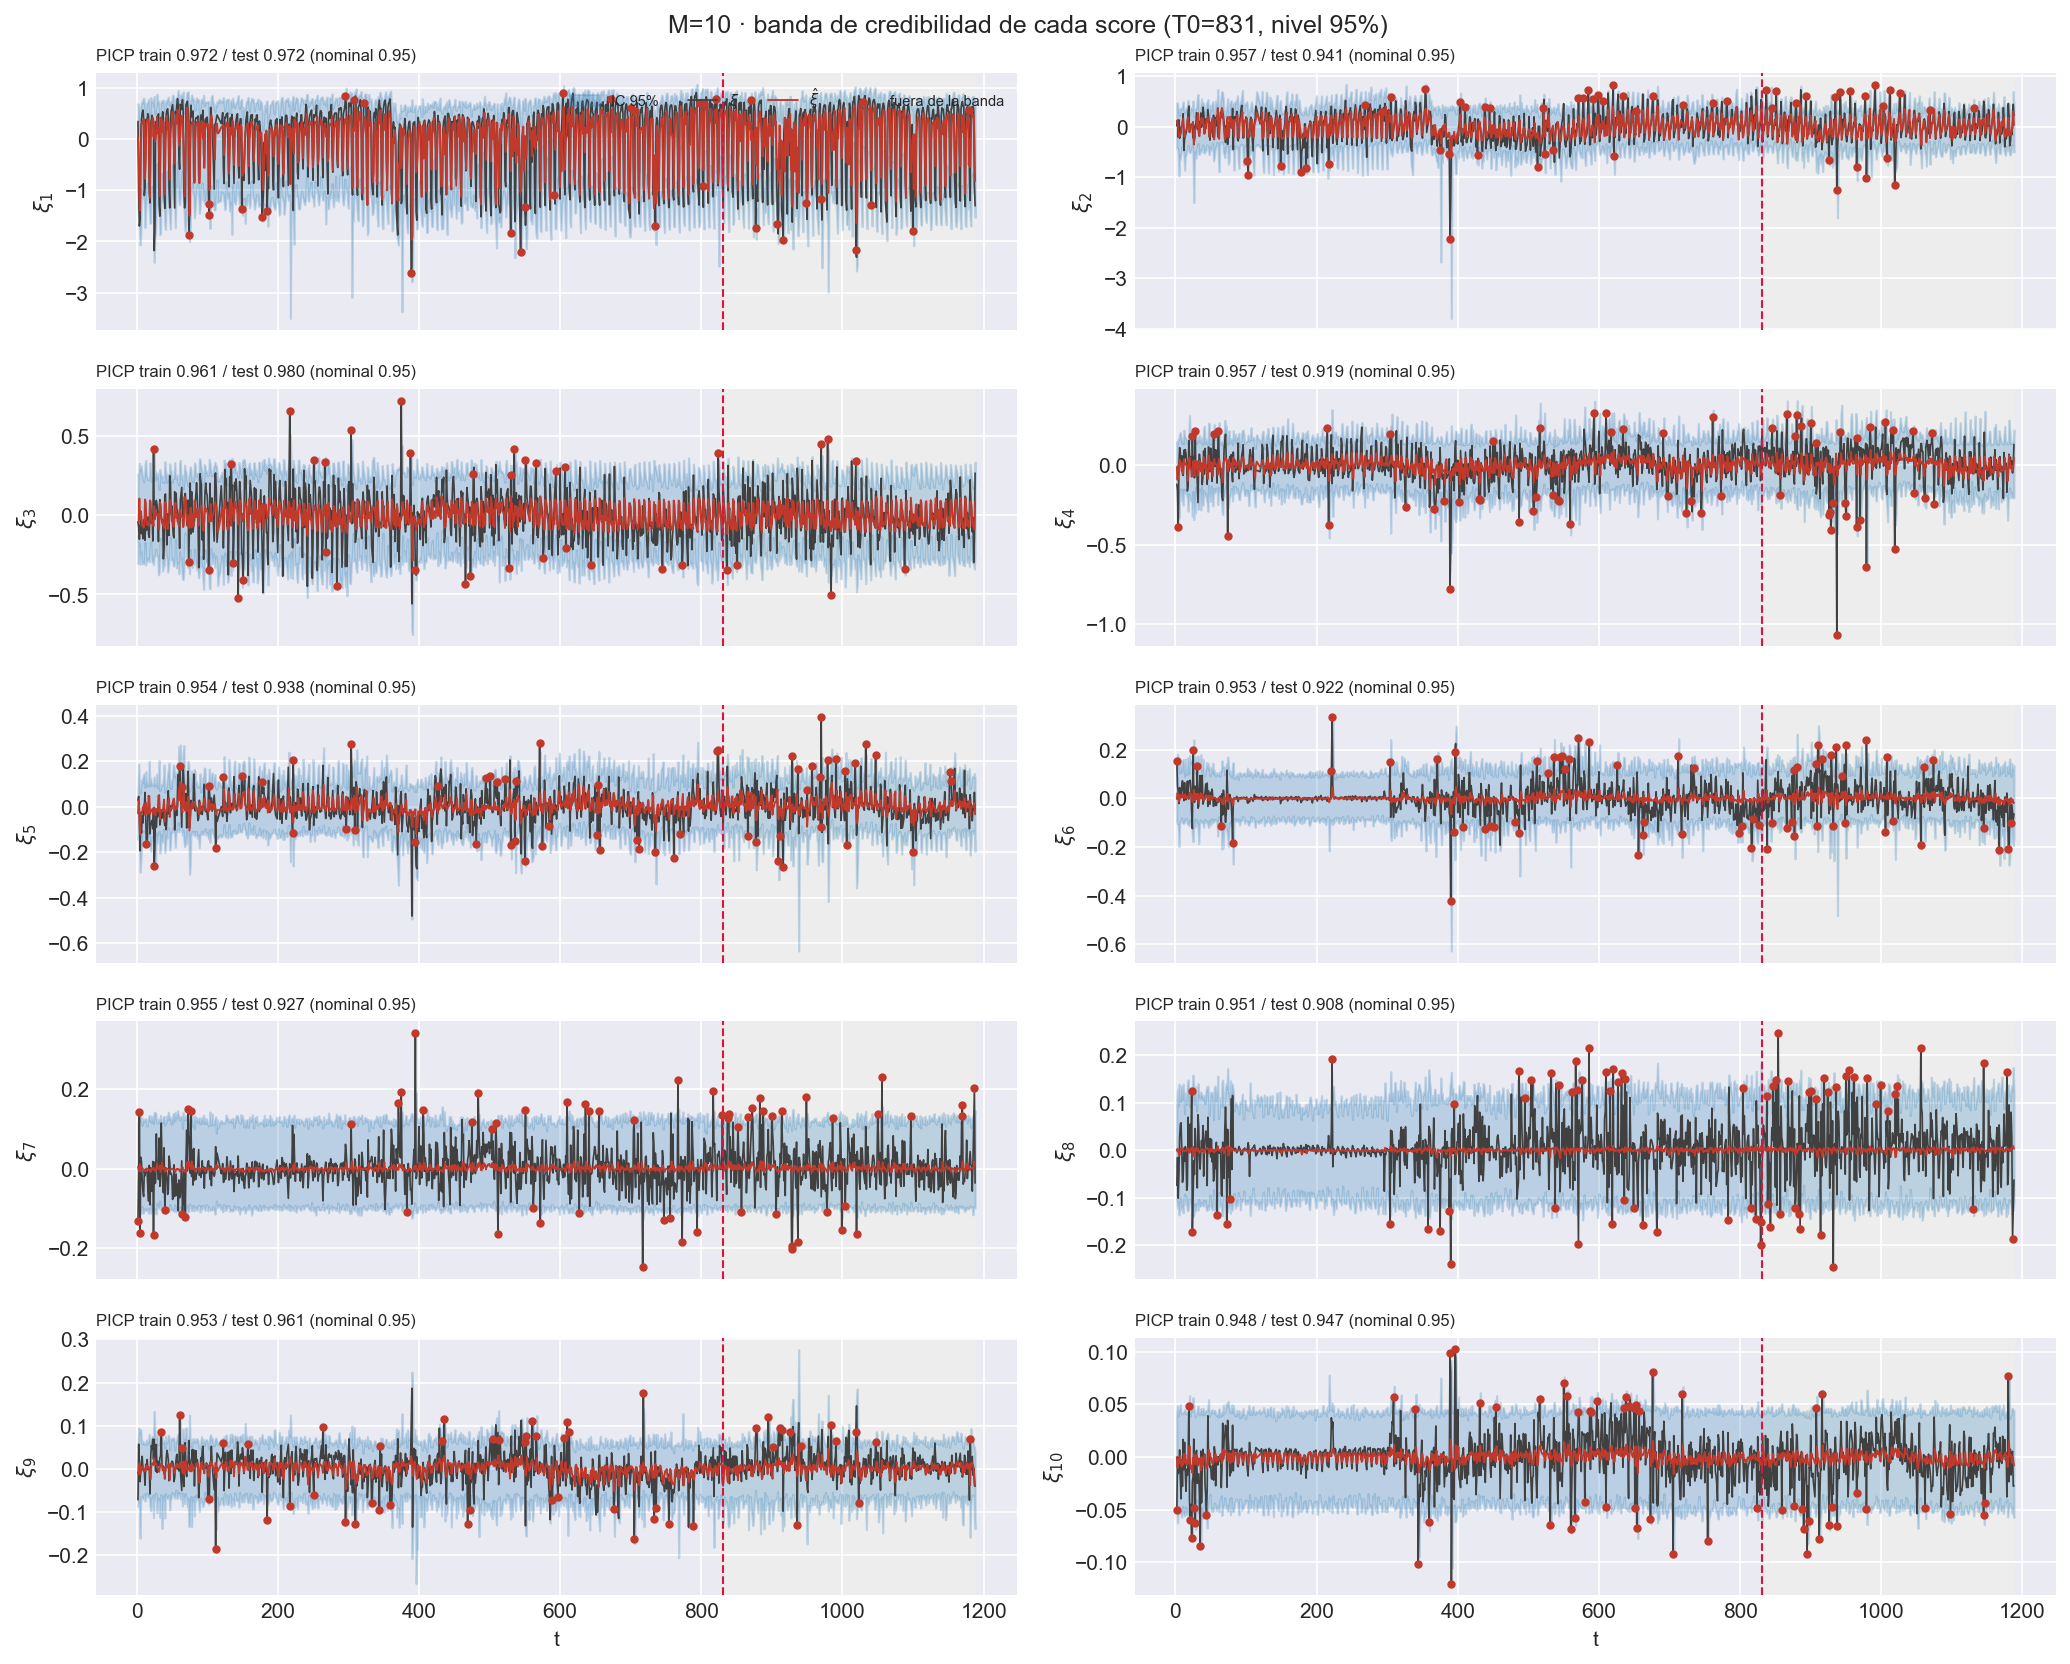
\includegraphics[width=\textwidth,height=0.75\textheight,keepaspectratio]{IMG/aneC_00/aneC_00_92_scores_banda_credibilidad_101.png}
\caption{Banda de credibilidad al 95\% de cada score, tráfico con rezago $\{1\}$ ($M = 10$).}
\label{fig:aneC_92_scores_banda_credibilidad_101}
\end{figure}

\begin{figure}[H]
\centering
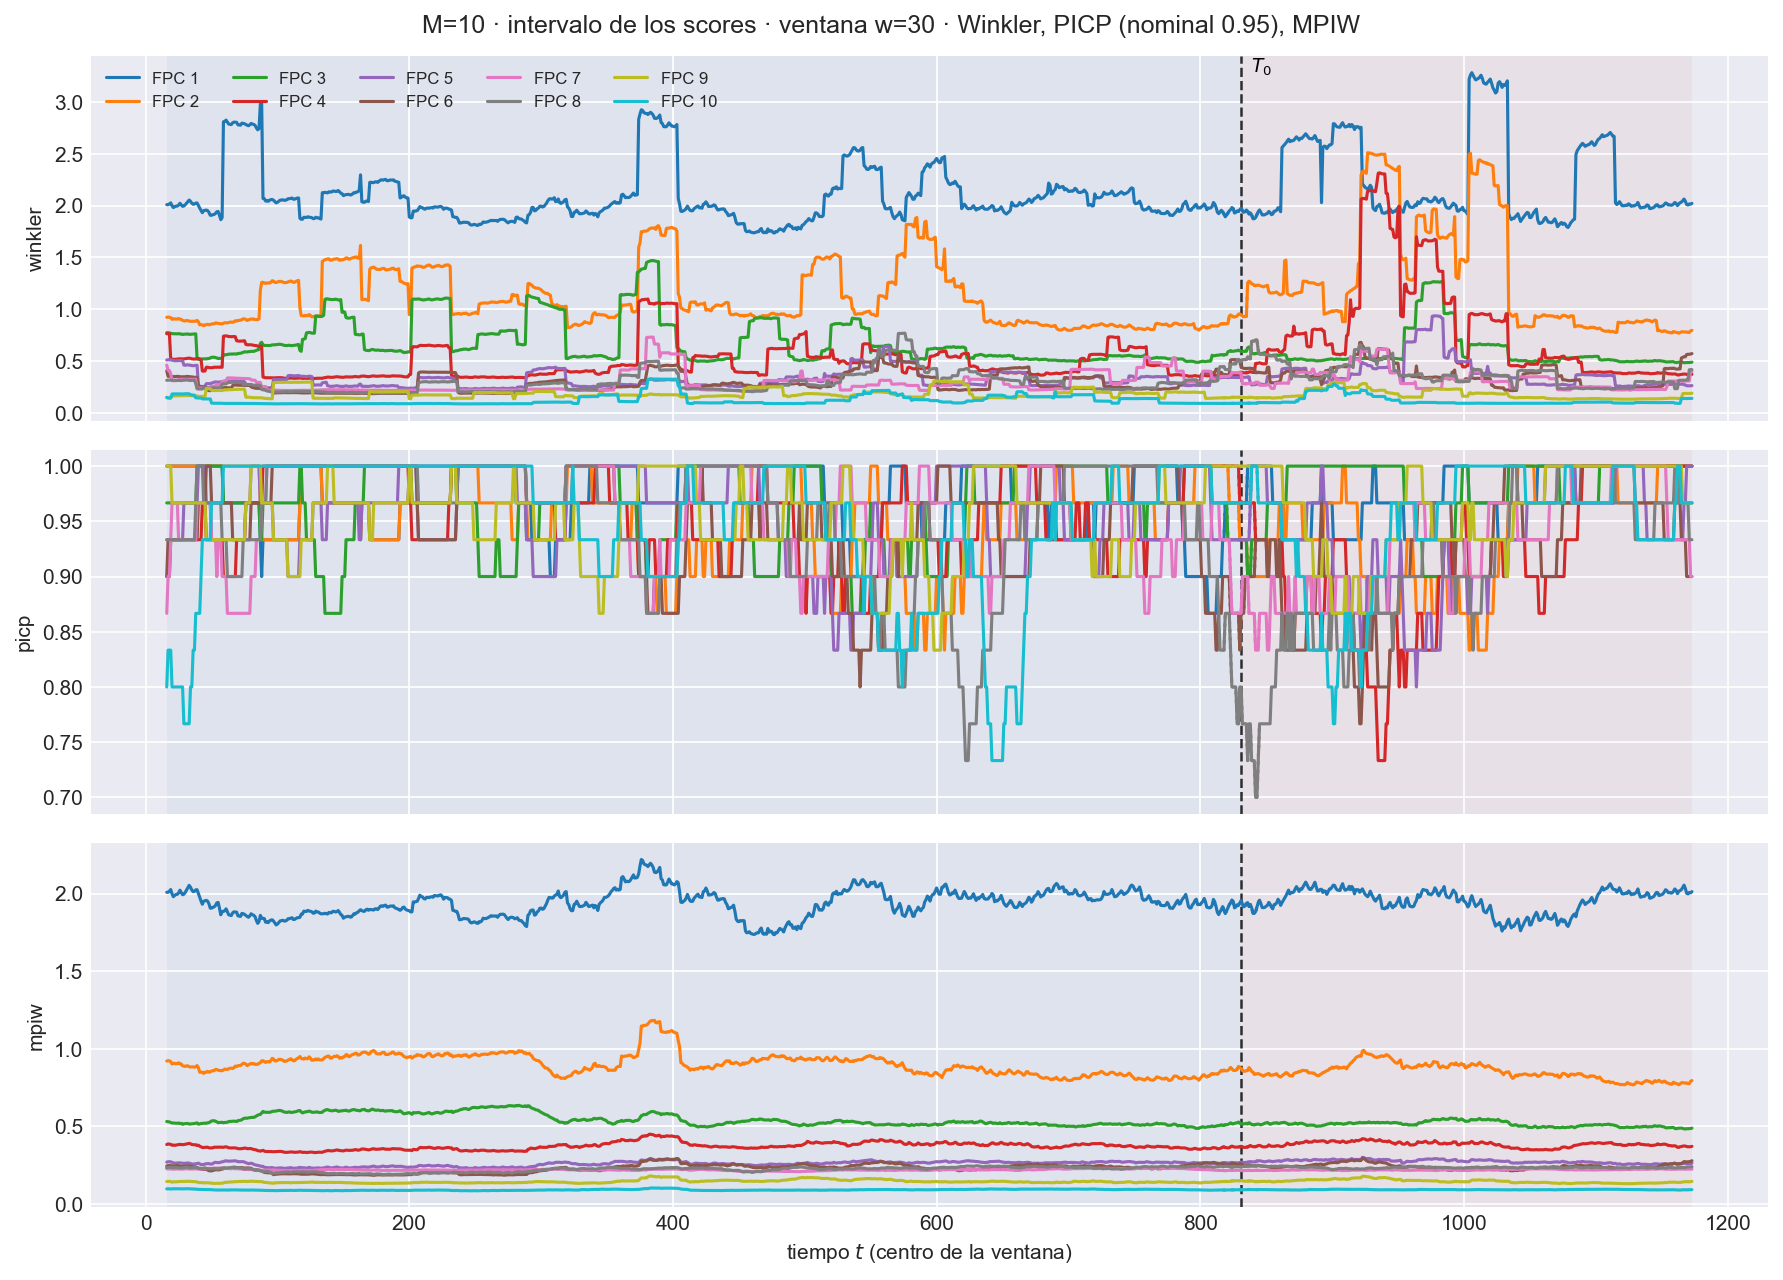
\includegraphics[width=\textwidth,height=0.75\textheight,keepaspectratio]{IMG/aneC_00/aneC_00_93_ventana_scores_intervalo_w30_101.png}
\caption{Métricas de intervalo de cada score sobre la ventana móvil, tráfico con rezago $\{1\}$ ($M = 10$).}
\label{fig:aneC_93_ventana_scores_intervalo_w30_101}
\end{figure}

\begin{figure}[H]
\centering
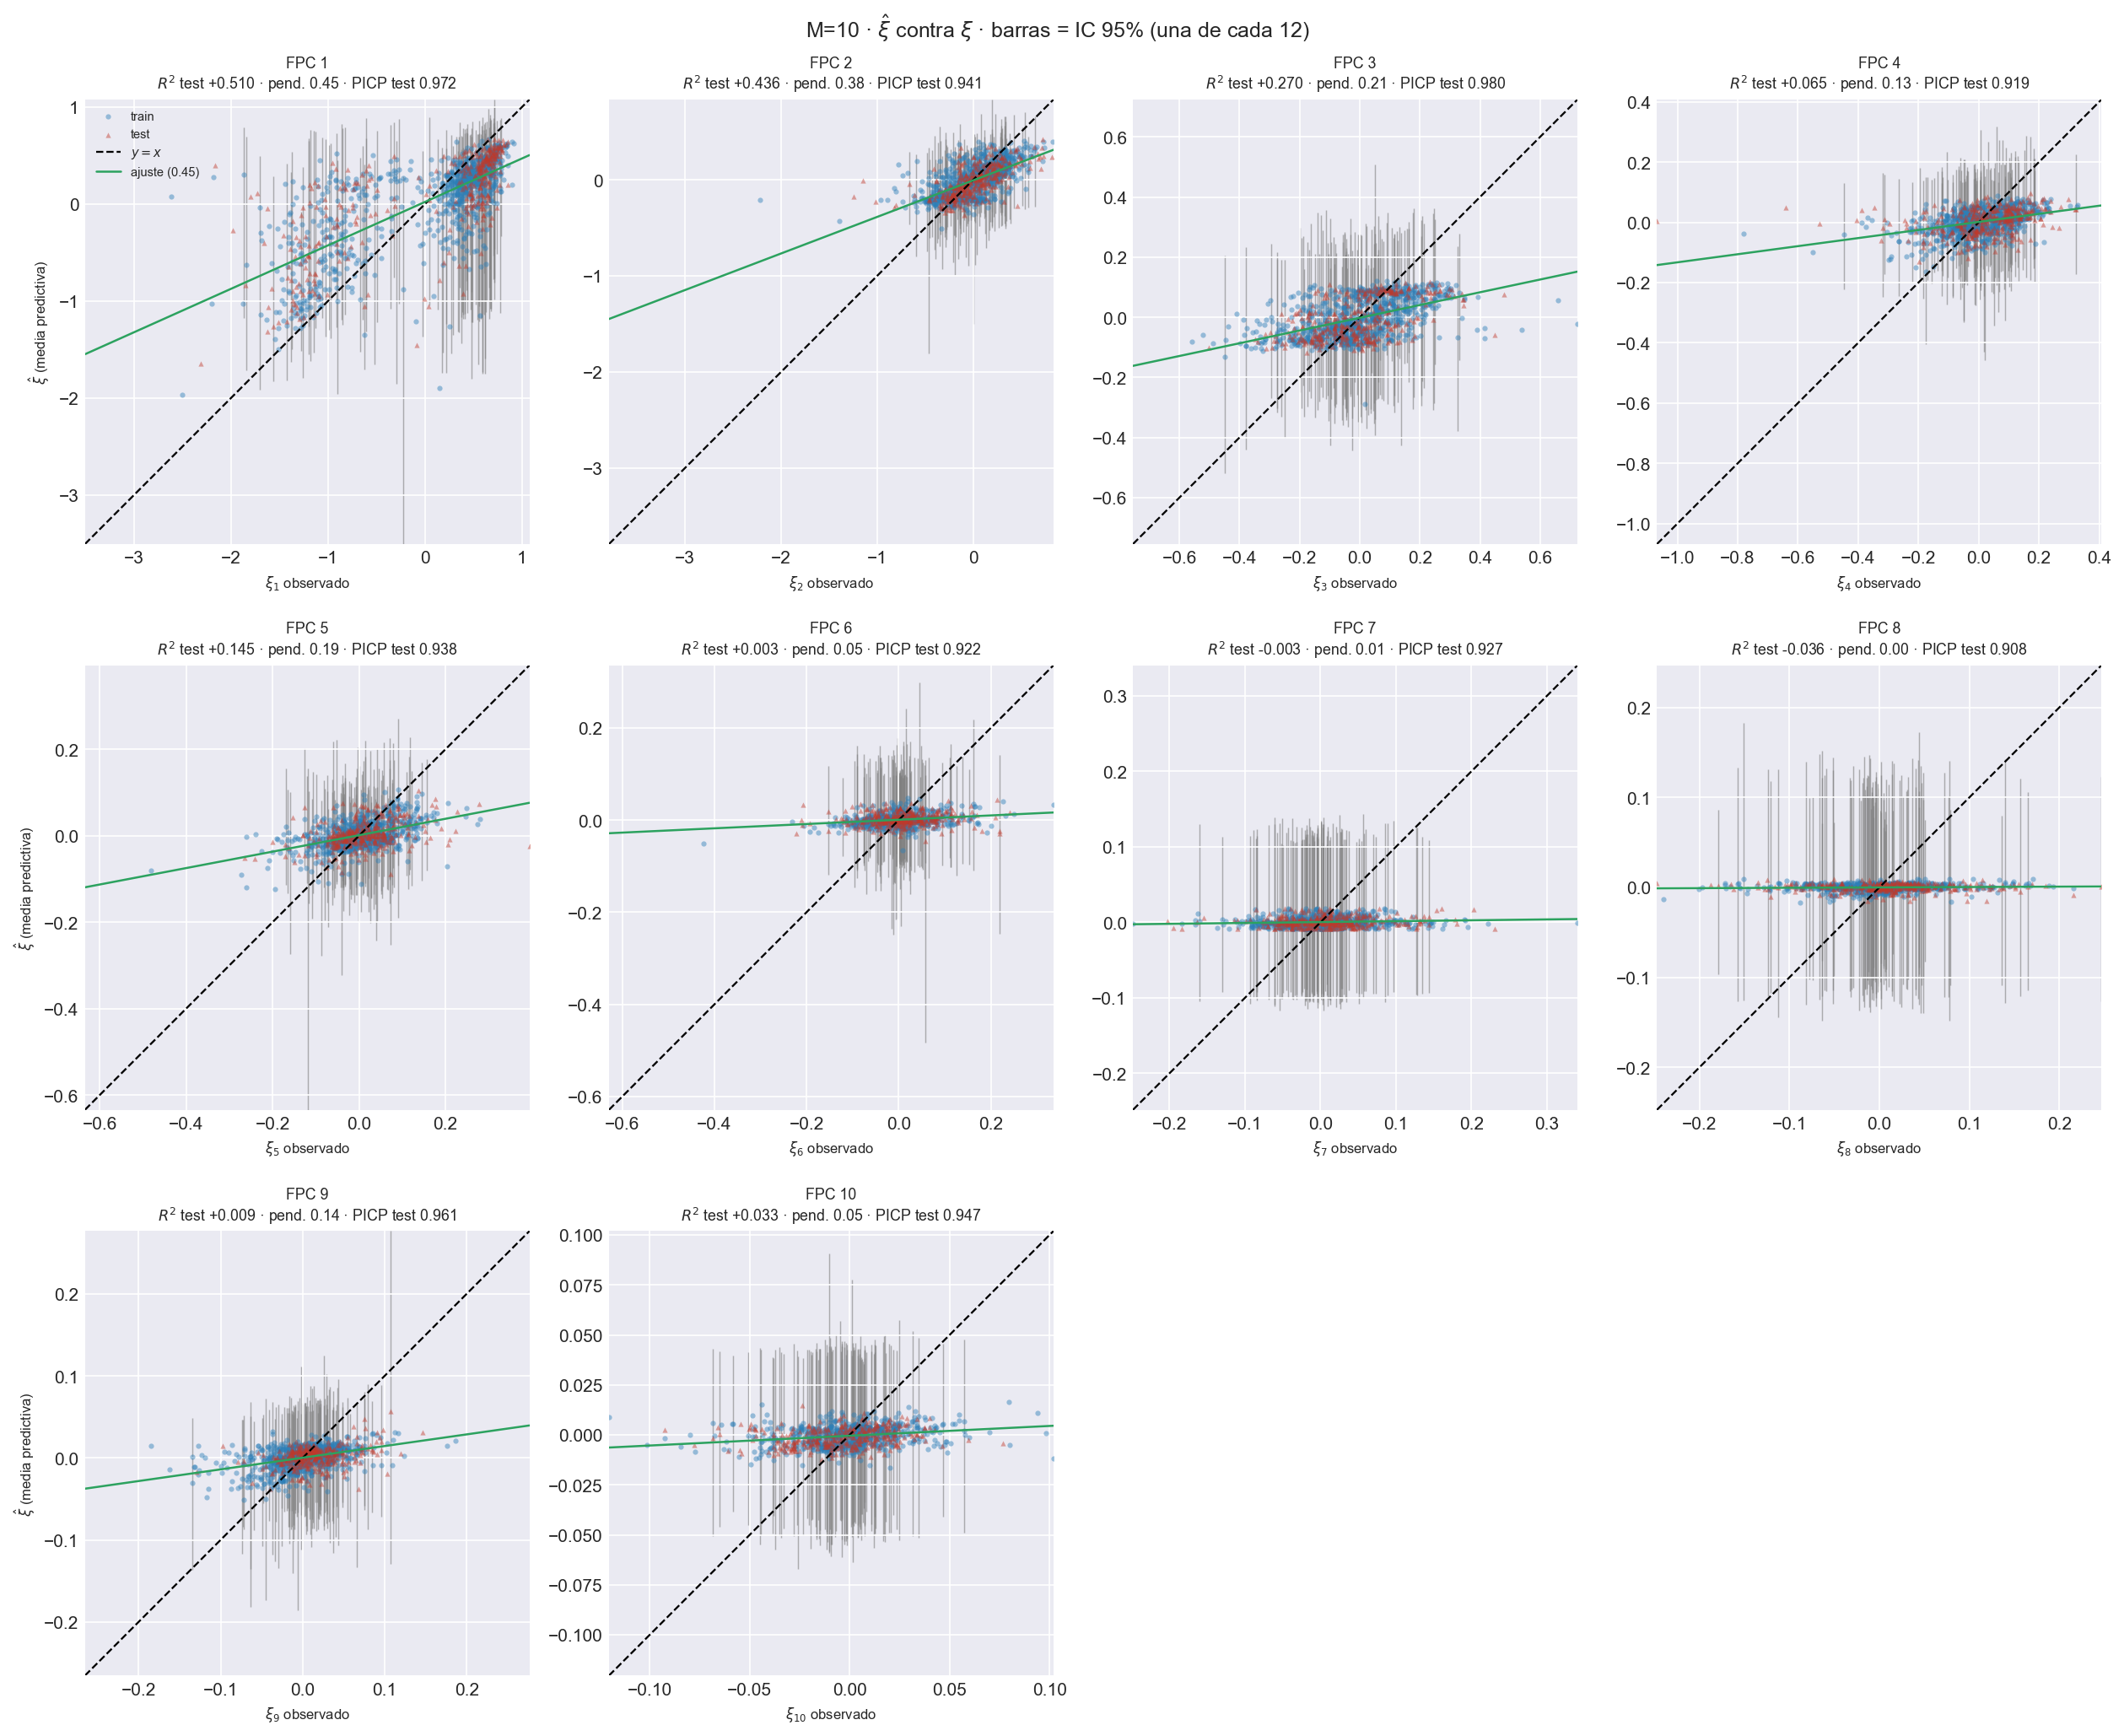
\includegraphics[width=\textwidth,height=0.75\textheight,keepaspectratio]{IMG/aneC_00/aneC_00_94_scores_dispersion_vs_real_101.png}
\caption{Dispersión estimada de cada score frente a la observada, tráfico con rezago $\{1\}$ ($M = 10$).}
\label{fig:aneC_94_scores_dispersion_vs_real_101}
\end{figure}

\begin{figure}[H]
\centering
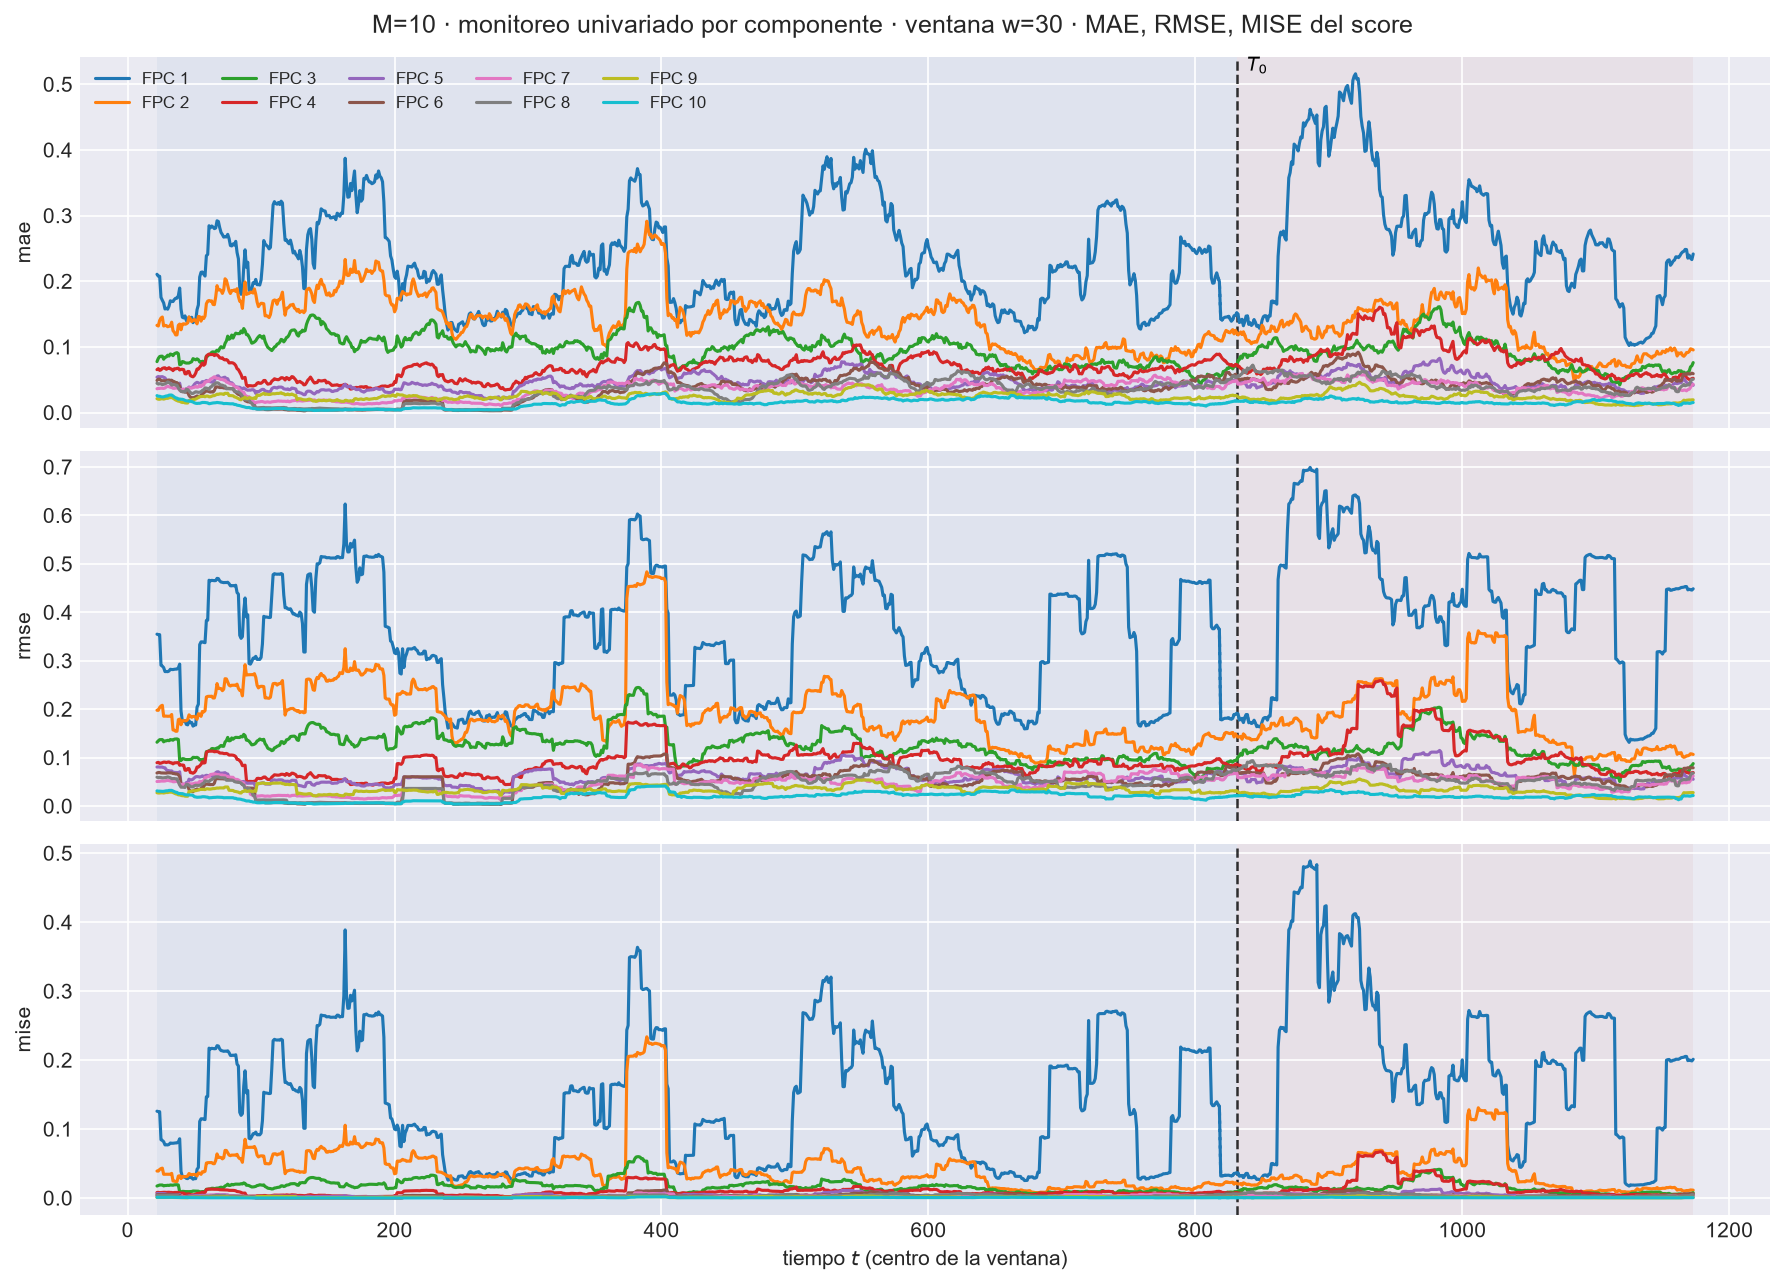
\includegraphics[width=\textwidth,height=0.75\textheight,keepaspectratio]{IMG/aneC_00/aneC_00_91_ventana_univariado_w30_102.png}
\caption{Error de cada score sobre la ventana móvil, tráfico con rezagos $\{1,7\}$ ($M = 10$).}
\label{fig:aneC_91_ventana_univariado_w30_102}
\end{figure}

\begin{figure}[H]
\centering
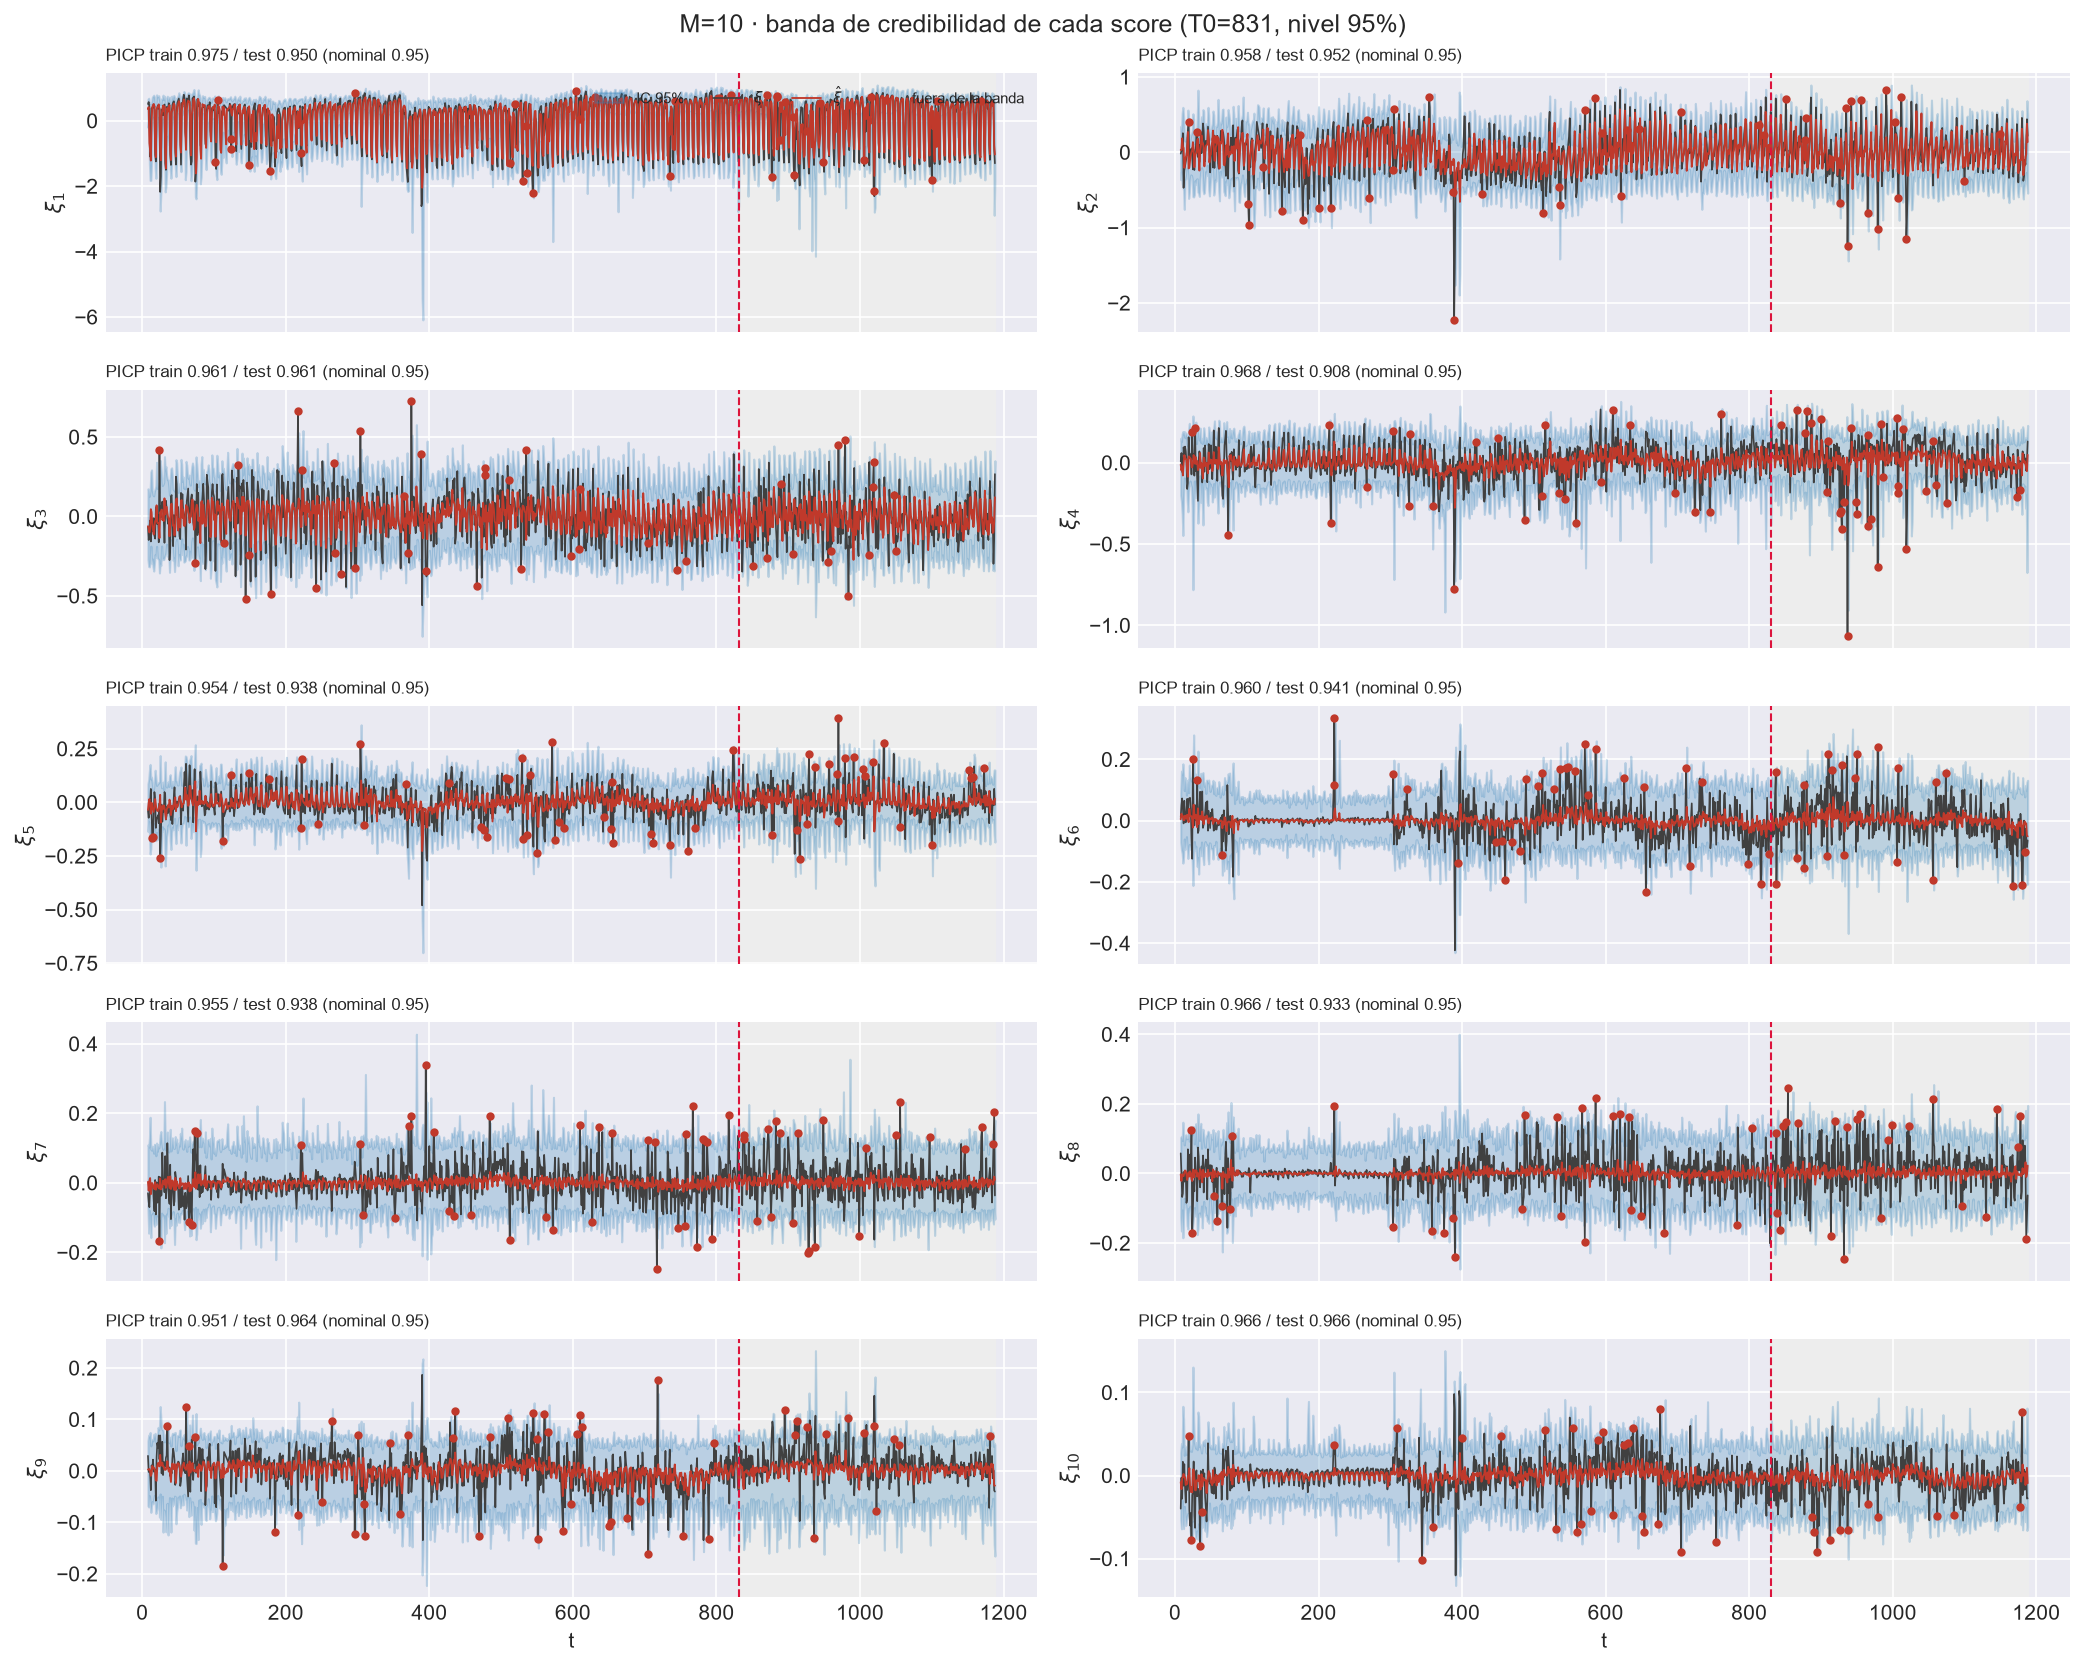
\includegraphics[width=\textwidth,height=0.75\textheight,keepaspectratio]{IMG/aneC_00/aneC_00_92_scores_banda_credibilidad_102.png}
\caption{Banda de credibilidad al 95\% de cada score, tráfico con rezagos $\{1,7\}$ ($M = 10$).}
\label{fig:aneC_92_scores_banda_credibilidad_102}
\end{figure}

\begin{figure}[H]
\centering
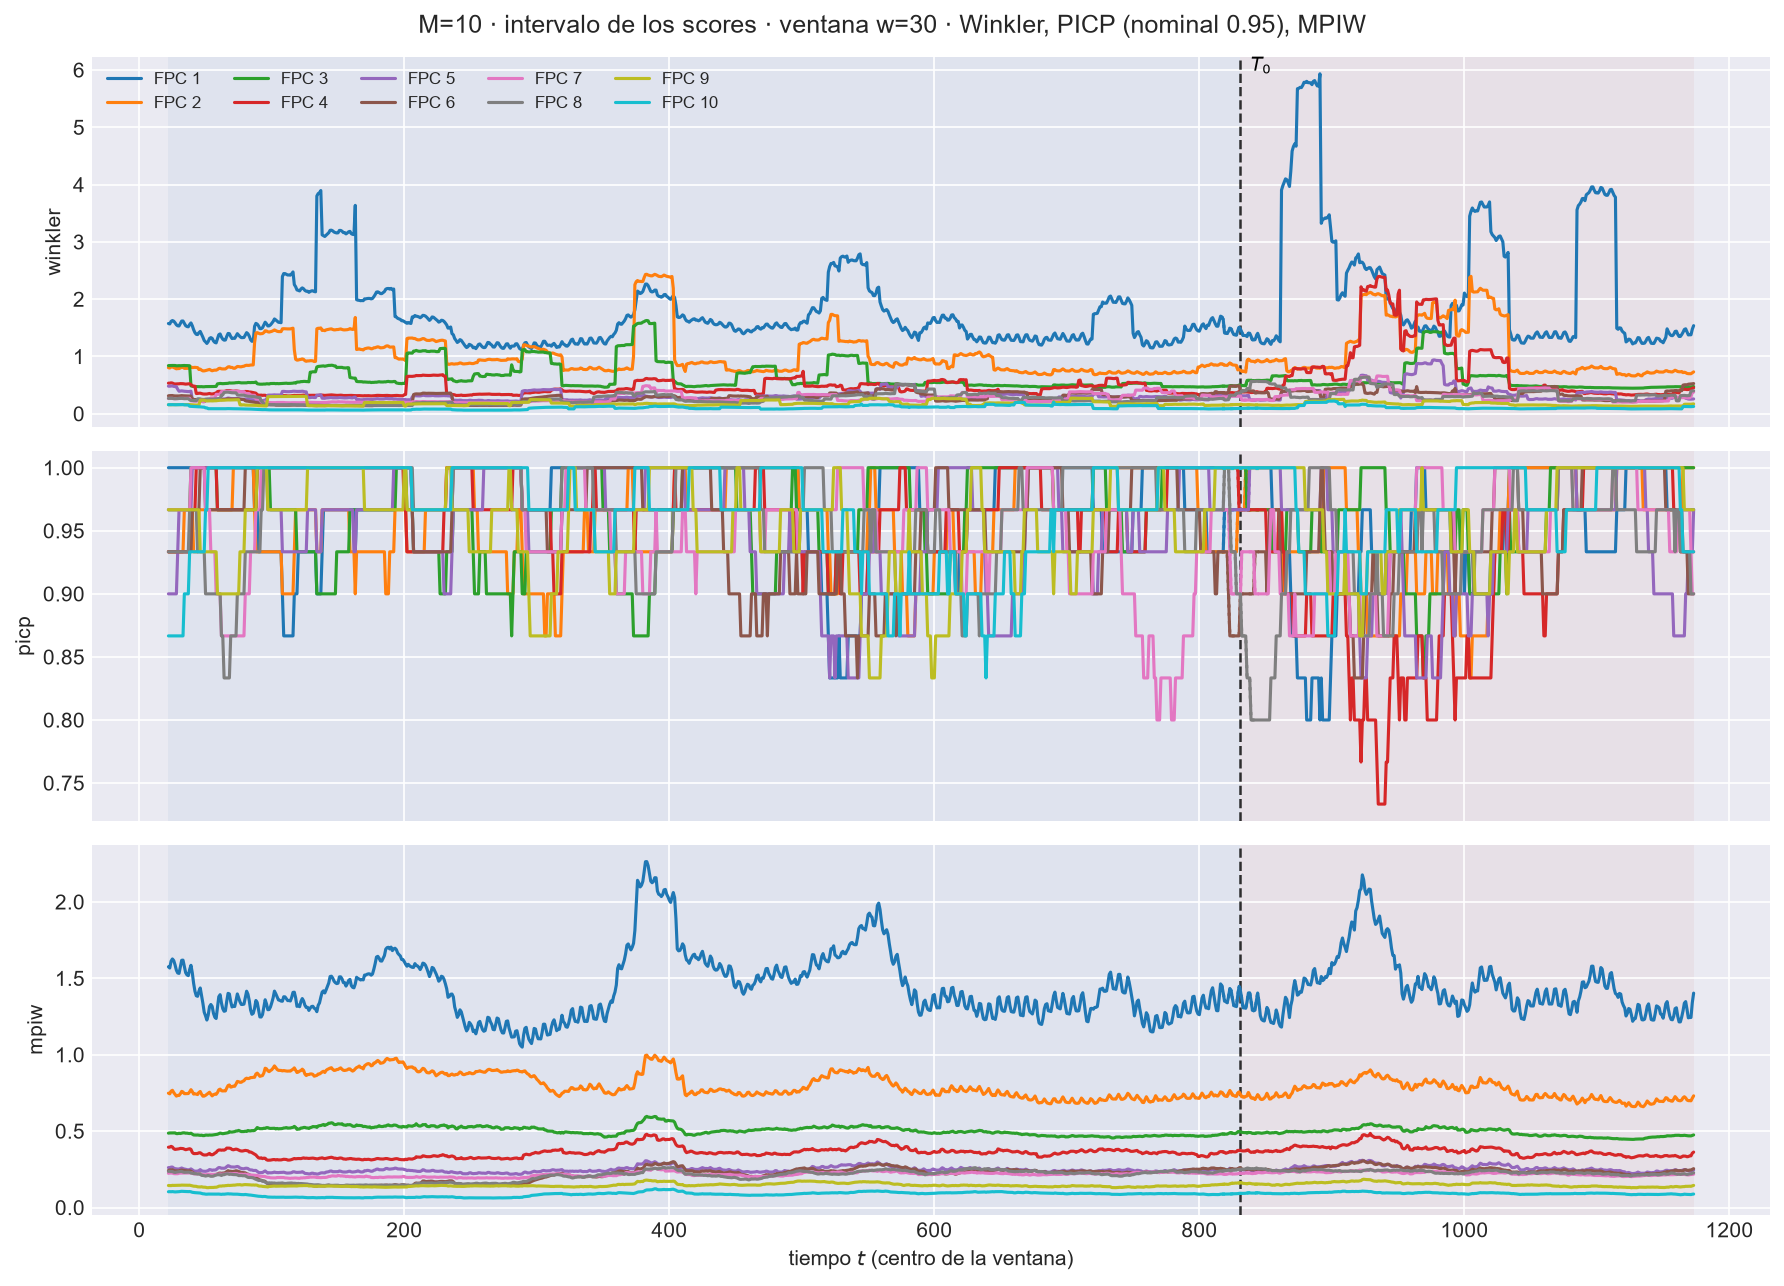
\includegraphics[width=\textwidth,height=0.75\textheight,keepaspectratio]{IMG/aneC_00/aneC_00_93_ventana_scores_intervalo_w30_102.png}
\caption{Métricas de intervalo de cada score sobre la ventana móvil, tráfico con rezagos $\{1,7\}$ ($M = 10$).}
\label{fig:aneC_93_ventana_scores_intervalo_w30_102}
\end{figure}

\begin{figure}[H]
\centering
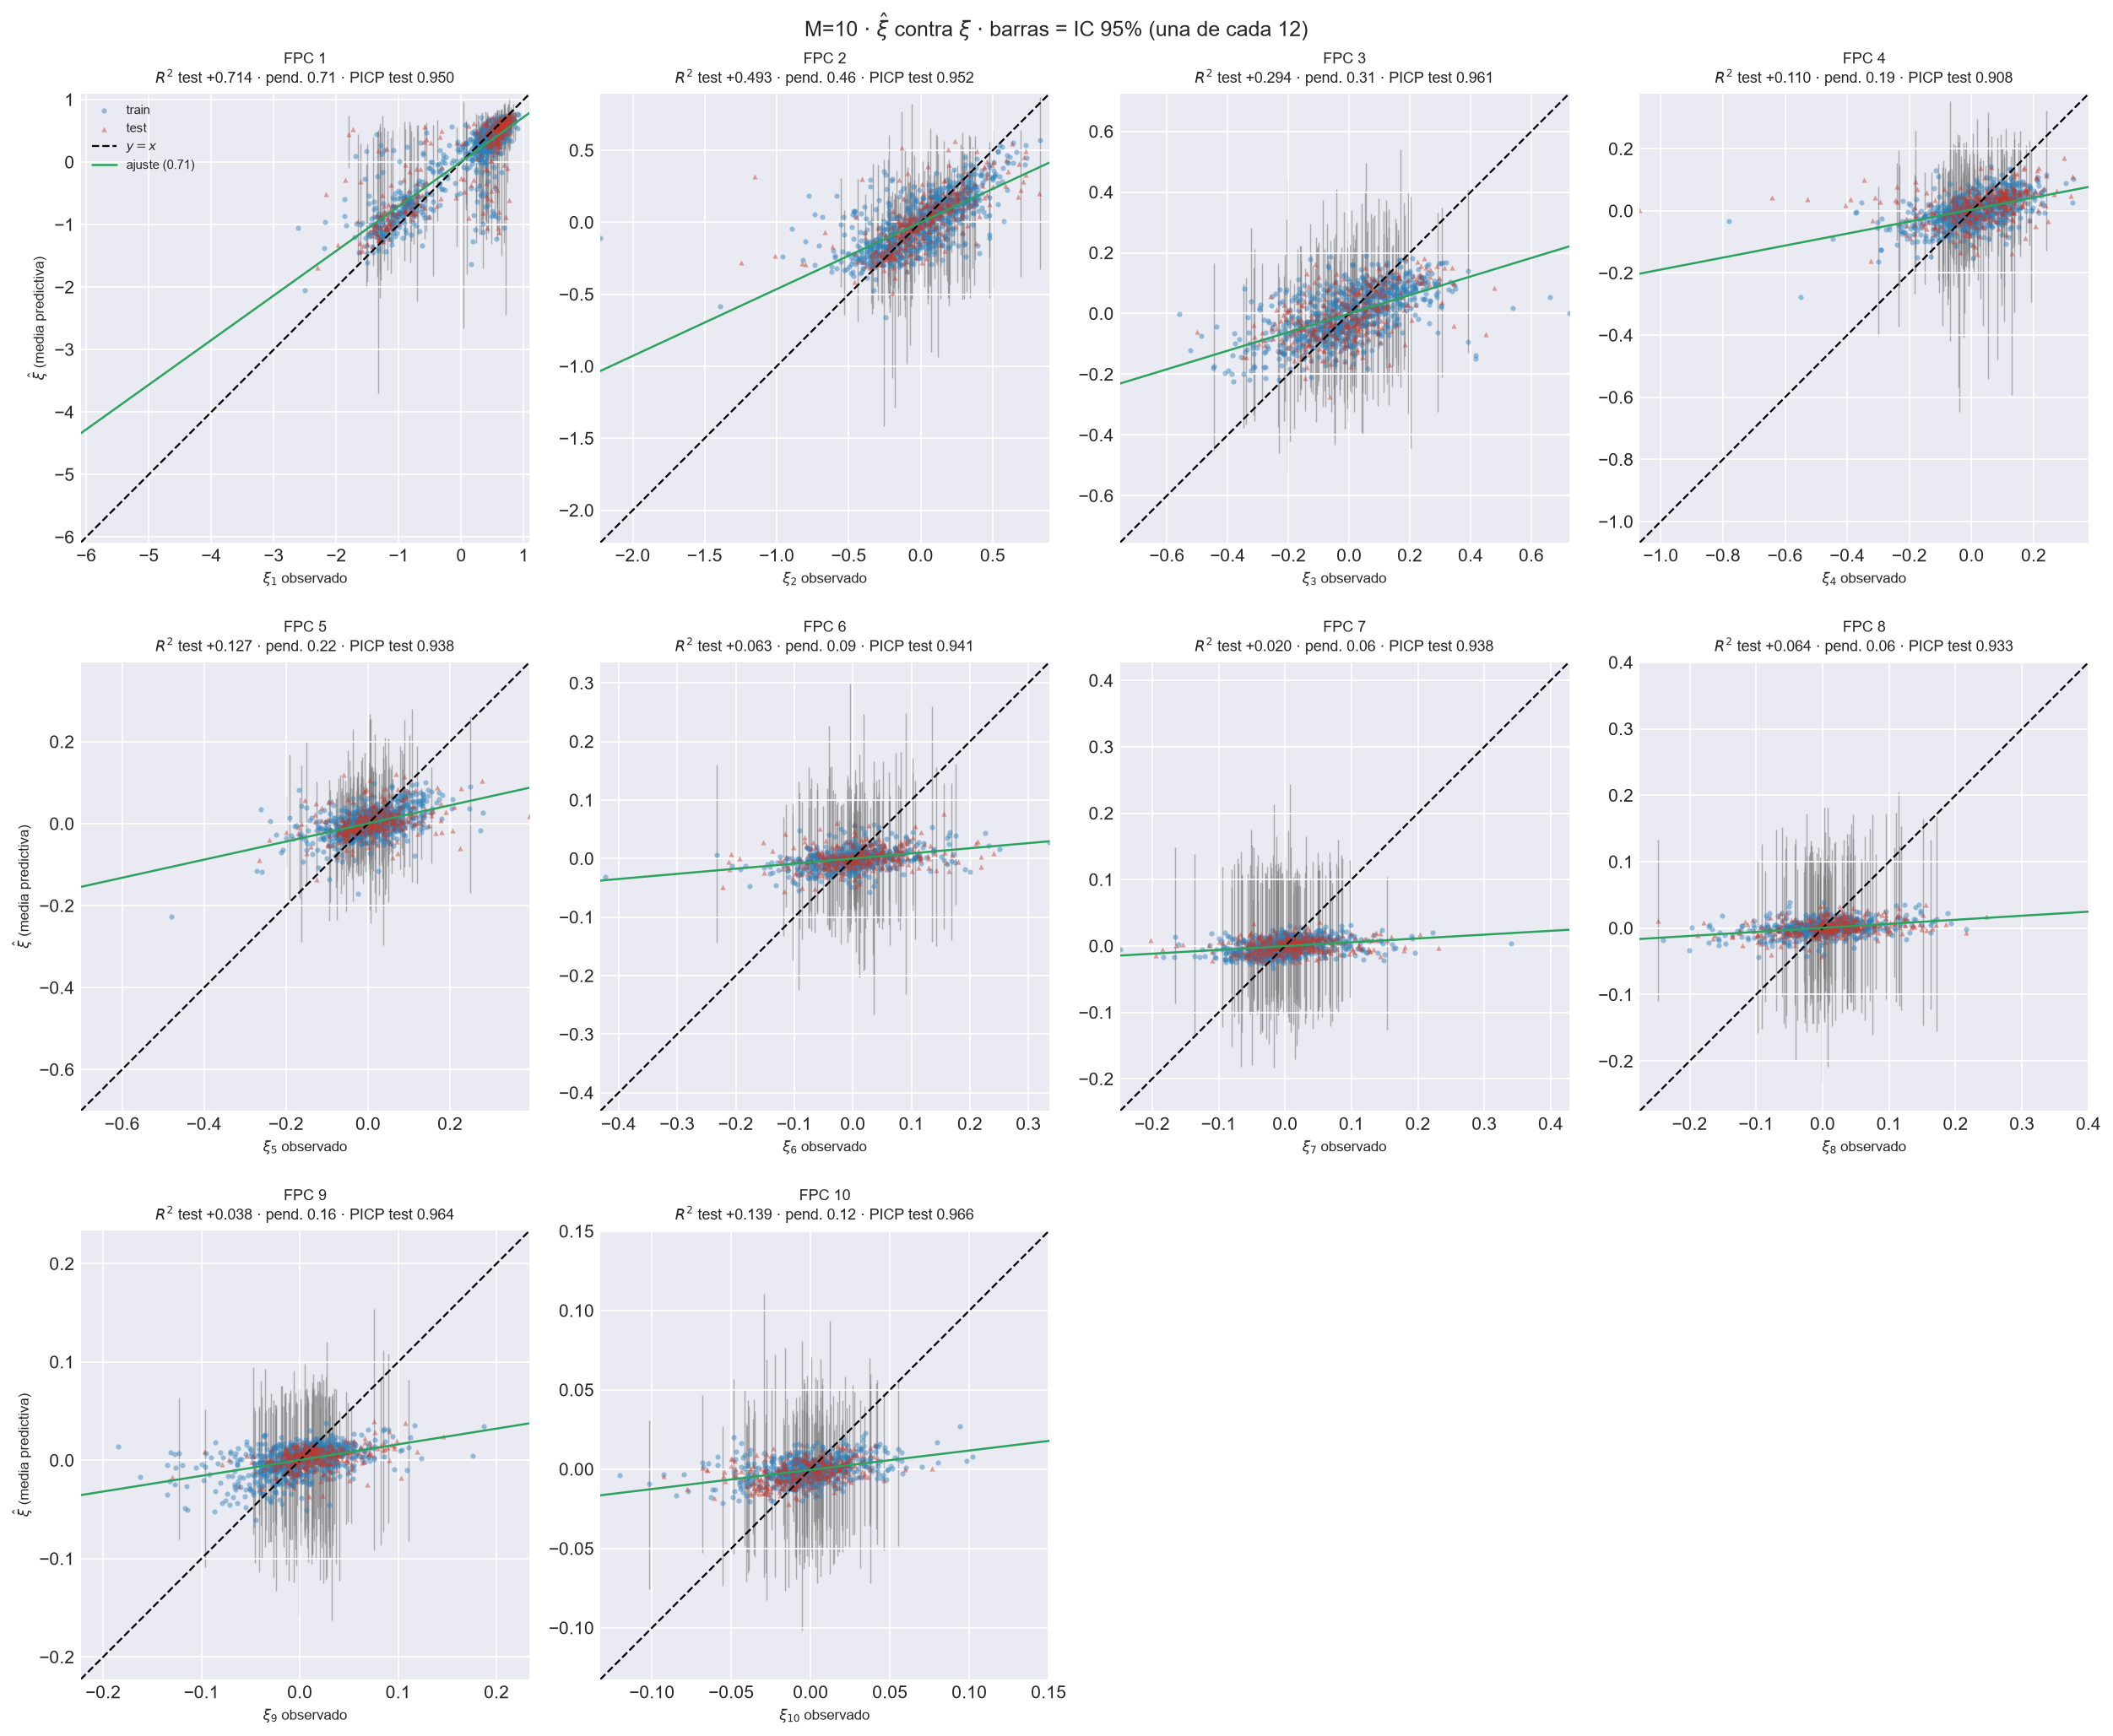
\includegraphics[width=\textwidth,height=0.75\textheight,keepaspectratio]{IMG/aneC_00/aneC_00_94_scores_dispersion_vs_real_102.png}
\caption{Dispersión estimada de cada score frente a la observada, tráfico con rezagos $\{1,7\}$ ($M = 10$).}
\label{fig:aneC_94_scores_dispersion_vs_real_102}
\end{figure}

\section{Selección de variables en los scores menores}
\label{aneC_00_09_seleccion}
% Autofunciones 1-4 y 5-10 (scratchpad figuras_pip.py) y PIP global con burn = 1000 (= 46_pip.csv del _03 de 101 y 102).

Complementa la Sección~\ref{04_03_05_seleccion} con las autofunciones de la FPCA y la ocupación de cada mezcla, que condiciona la lectura de la PIP.

\begin{figure}[H]
\centering
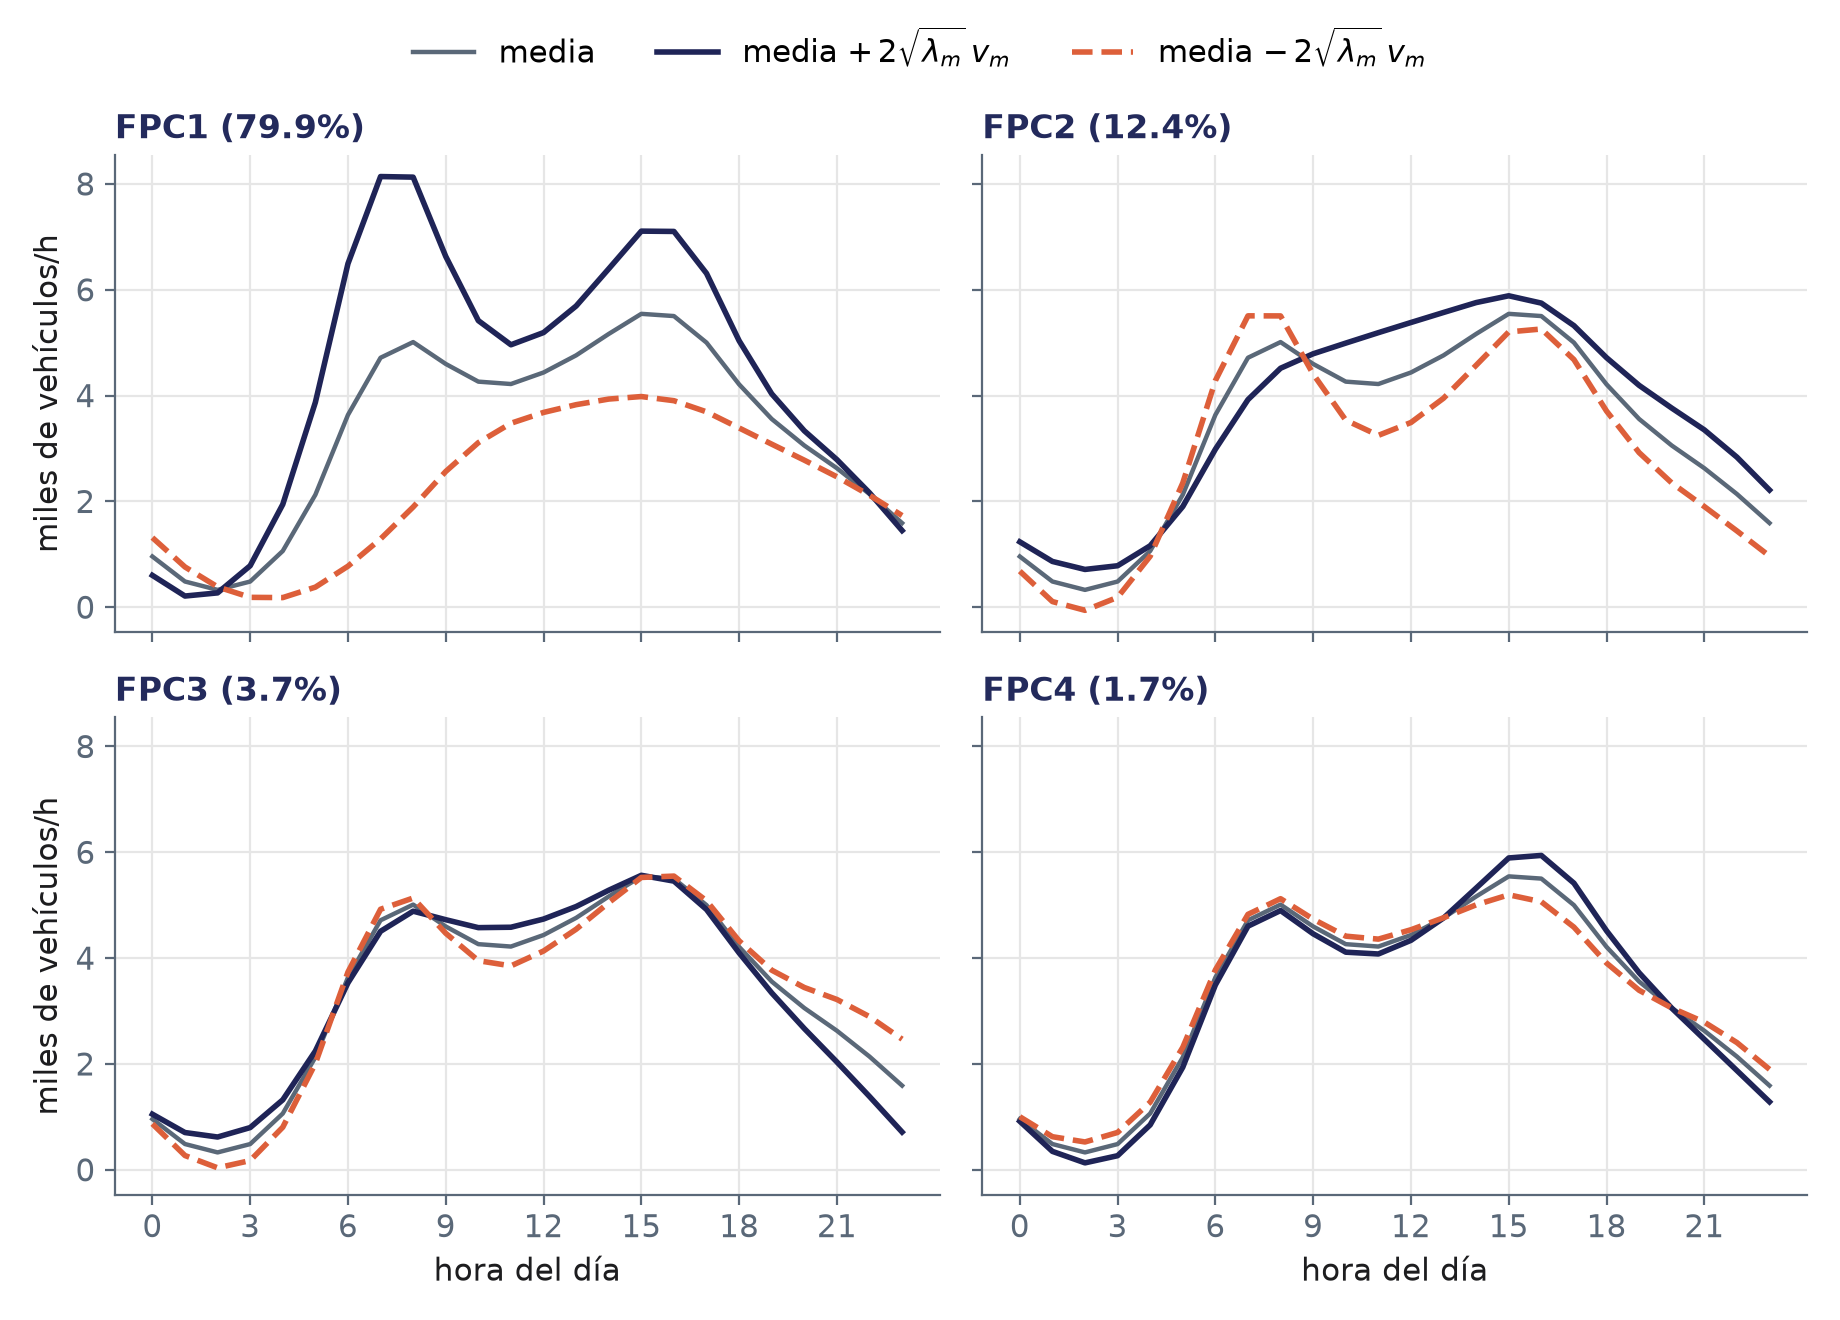
\includegraphics[width=\textwidth,height=0.45\textheight,keepaspectratio]{IMG/aneC_00/aneC_00_autofunciones.png}
\caption{Curva media del bloque de entrenamiento y su perturbación $\mu \pm 2\sqrt{\lambda_m}\,v_m$ a lo largo de las cuatro primeras autofunciones, con la fracción de varianza que explica cada una.}
\label{fig:aneC_autofunciones}
\end{figure}

\begin{figure}[H]
\centering
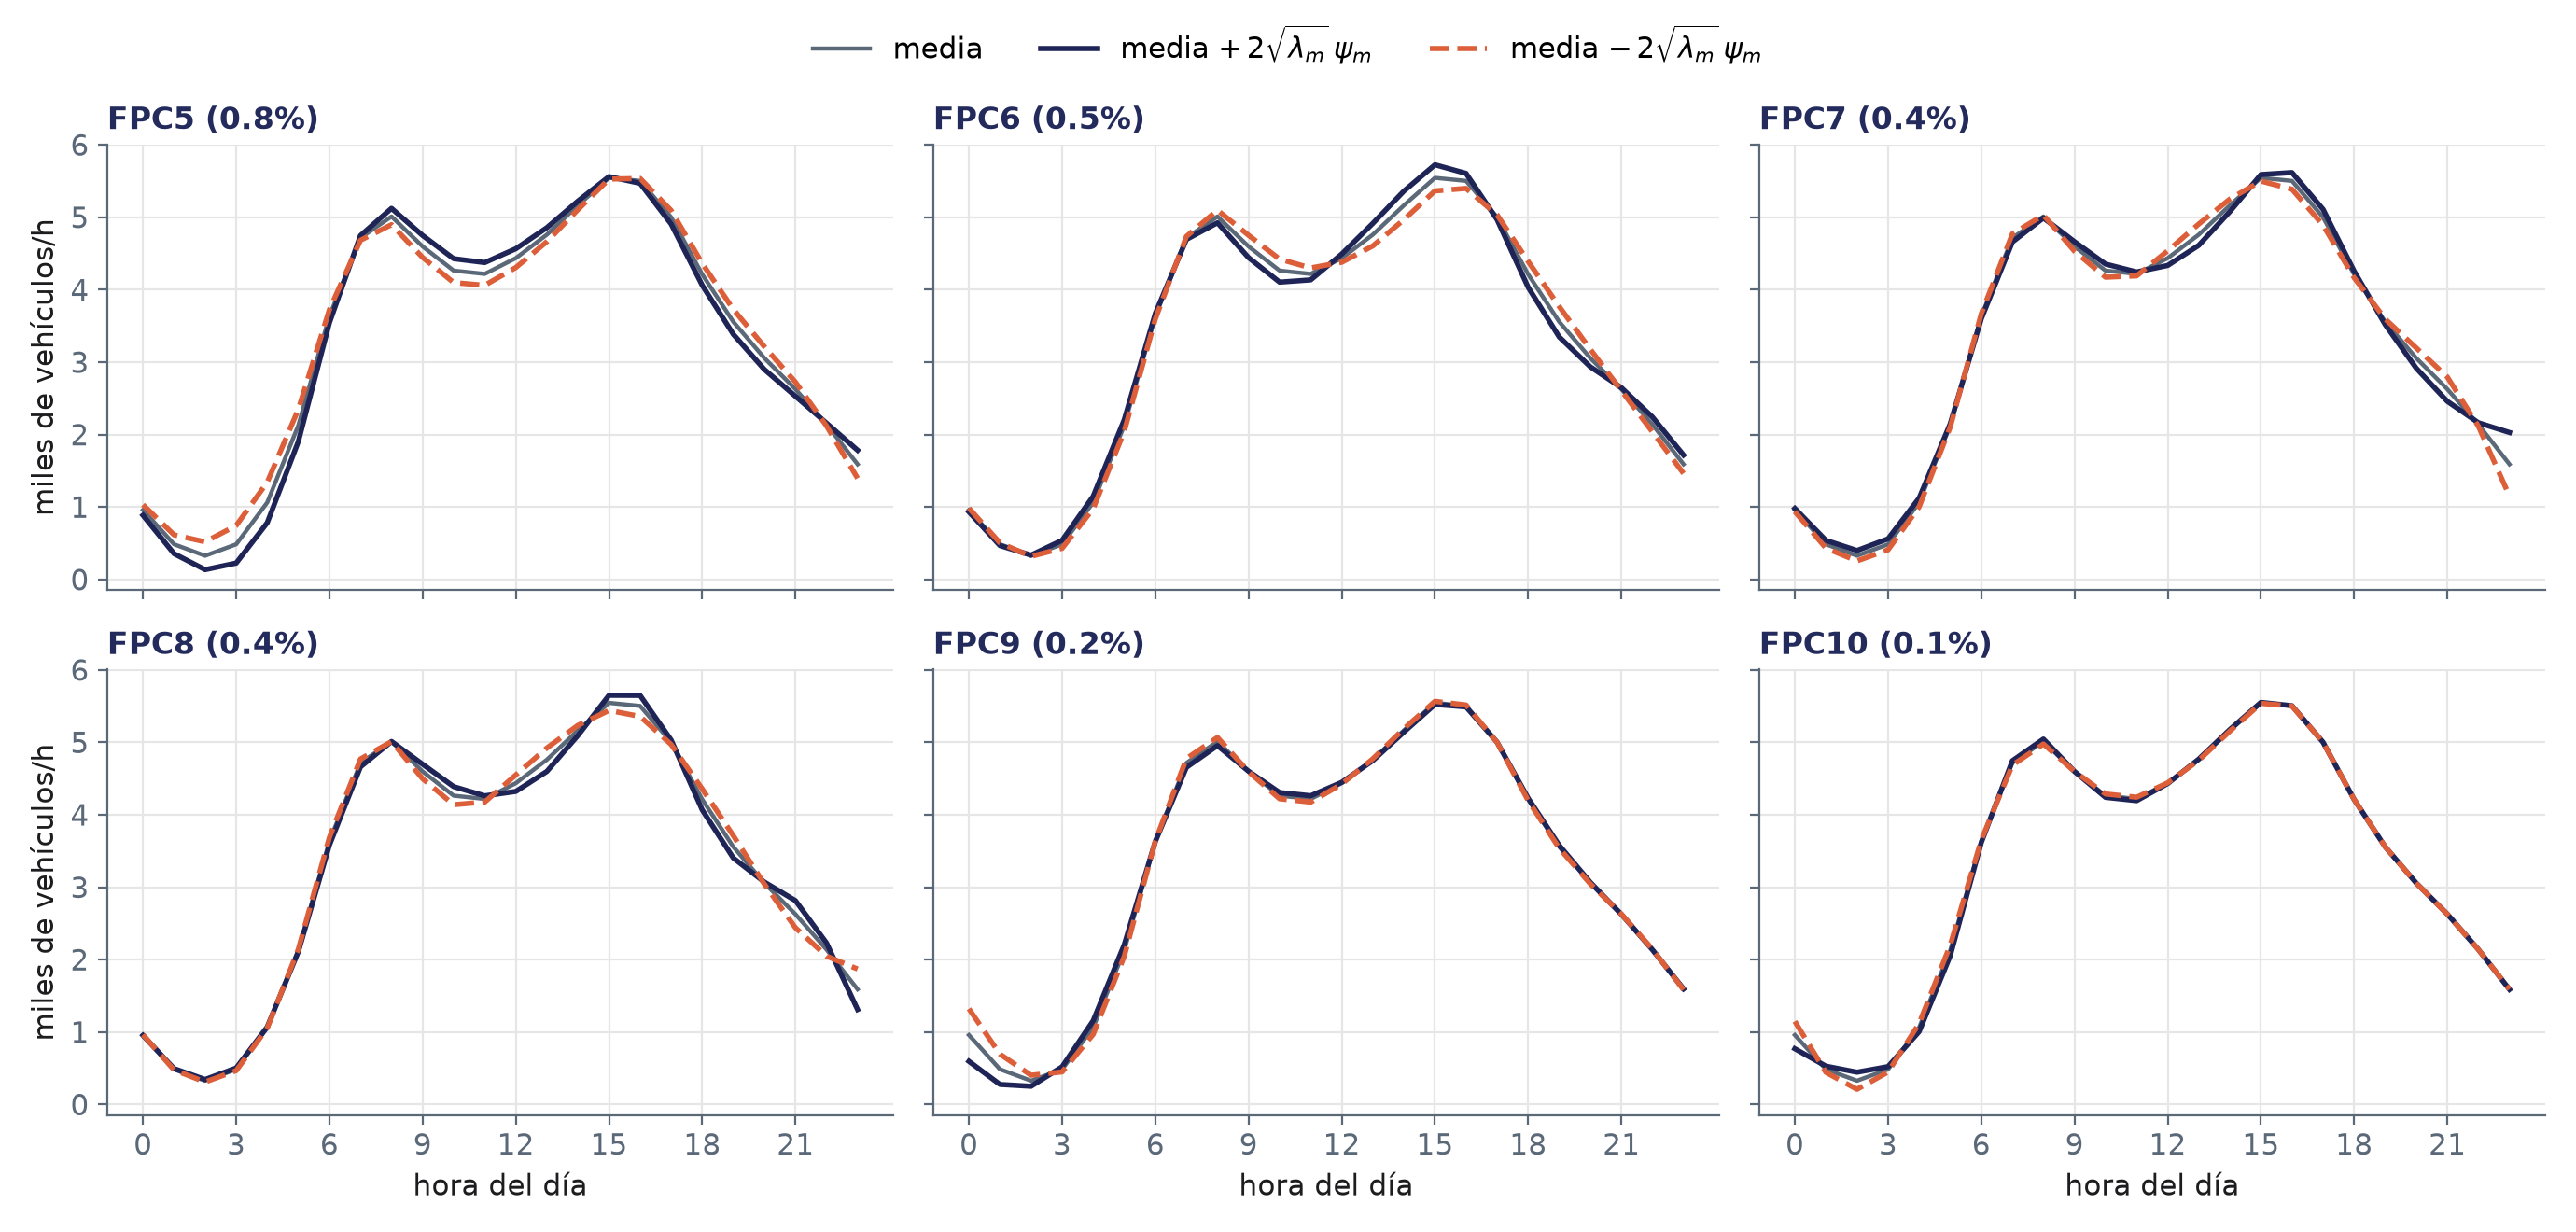
\includegraphics[width=\textwidth,height=0.6\textheight,keepaspectratio]{IMG/aneC_00/aneC_00_autofunciones_menores.png}
\caption{Curva media del bloque de entrenamiento y su perturbación $\mu \pm 2\sqrt{\lambda_m}\,v_m$ a lo largo de las autofunciones $5$ a $10$.}
\label{fig:aneC_autofunciones_menores}
\end{figure}

Las autofunciones menores (Figura~\ref{fig:aneC_autofunciones_menores}) son ajustes locales del perfil, de una amplitud de unos cientos de vehículos por hora frente a los miles de las cuatro primeras (Figura~\ref{fig:aneC_autofunciones}). La quinta mueve la madrugada, entre la una y las cinco, frente a la media mañana; la sexta desplaza la punta de la tarde hacia antes o después de las dieciséis horas; la séptima y la octava ajustan el cierre de la tarde y la noche, y la novena y la décima se concentran en las primeras horas del día, en el borde del dominio.

\begin{table}[H]
\centering\small
\setlength{\tabcolsep}{4pt}
\caption{Ocupación de la mezcla y selección de cada score ($M = 10$): fracción de la varianza, índice medio del último átomo ocupado ($N_1$, sobre 30), número de covariables con PIP mayor que $0.5$ y PIP mínima, con rezago $\{1\}$ (diez covariables) y rezagos $\{1,7\}$ (diez de cada rezago).}
\label{tab:aneC_pip}
\begin{tabular}{l c ccc cccc}
\hline
 & & \multicolumn{3}{c}{Rezago $\{1\}$} & \multicolumn{4}{c}{Rezagos $\{1,7\}$} \\
 & & & \multicolumn{2}{c}{PIP} & & \multicolumn{3}{c}{PIP} \\
Score & Var. (\%) & $N_1$ & $> 0.5$ & mín. & $N_1$ & $> 0.5$, $t-1$ & $> 0.5$, $t-7$ & mín. \\
\hline
$\xi_{t1}$  & 79.9 & 8.7  & 5 & 0.06 & 10.3 & 4  & 2  & 0.10 \\
$\xi_{t2}$  & 12.4 & 15.2 & 4 & 0.16 & 15.3 & 5  & 3  & 0.41 \\
$\xi_{t3}$  & 3.7  & 14.5 & 3 & 0.10 & 19.5 & 10 & 10 & 0.67 \\
$\xi_{t4}$  & 1.7  & 16.4 & 7 & 0.32 & 20.7 & 8  & 9  & 0.47 \\
$\xi_{t5}$  & 0.8  & 16.8 & 5 & 0.31 & 10.0 & 3  & 4  & 0.29 \\
$\xi_{t6}$  & 0.5  & 22.3 & 2 & 0.12 & 29.9 & 10 & 10 & 0.94 \\
$\xi_{t7}$  & 0.4  & 24.7 & 2 & 0.09 & 28.2 & 10 & 10 & 0.81 \\
$\xi_{t8}$  & 0.4  & 27.9 & 2 & 0.04 & 30.0 & 10 & 10 & 0.91 \\
$\xi_{t9}$  & 0.2  & 21.4 & 6 & 0.31 & 23.1 & 10 & 10 & 0.75 \\
$\xi_{t10}$ & 0.1  & 14.2 & 2 & 0.14 & 29.1 & 10 & 10 & 0.86 \\
\hline
\end{tabular}
\end{table}

El Cuadro~\ref{tab:aneC_pip} separa dos situaciones. Con el rezago de un día las mezclas de los scores menores son escasas aunque ocupen muchos átomos, pues las de los scores $6$, $7$, $8$ y $10$ incluyen solo dos covariables, su propio rezago y el de un score principal (el cuarto en el sexto, el primero en el séptimo y el octavo, y el tercero en el décimo), y dejan las demás en $0.47$ o menos. Con el rezago semanal, en cambio, las mezclas del tercer score y de los scores $6$ a $10$ ocupan entre 20 y 30 átomos y todas sus covariables superan $0.5$, con mínimos entre $0.67$ y $0.94$. La selección escasa se conserva solo en las mezclas que usan pocos átomos, las de los scores $1$, $2$ y $5$, con $N_1$ entre 10 y 15. La PIP de las mezclas que llenan el truncamiento refleja el número de átomos ocupados más que la relevancia de cada covariable, y por eso no se interpreta.
